\section{Casi d'uso}
\subsection{Classificazione dei casi d'uso}
I casi d'uso sono classificati secondo la seguente notazione:
\begin{center}
	UC[Codice padre].[Codice identificativo]
\end{center}
dove:
\begin{itemize}
	\item \textbf{codice padre:} indica il codice numerico in forma gerarchica del caso d'uso da cui deriva, viene omesso se non identificabile;
	\item \textbf{codice identificativo:} indica il codice numerico del caso d'uso.
\end{itemize}
\subsection{Attori}
Il sistema prevede come unico attore l'utente, ovvero l'agente assicuratore, già autenticato nel sistema, come da accordi presi con il proponente.
\subsection{Panoramica generale}
Per facilitare la consultazione dei casi d'uso, viene fornita un'immagine riassuntiva (non in notazione UML) che descrive le principali funzionalità offerte dall'applicazione.
\begin{figure}[H]
\centering
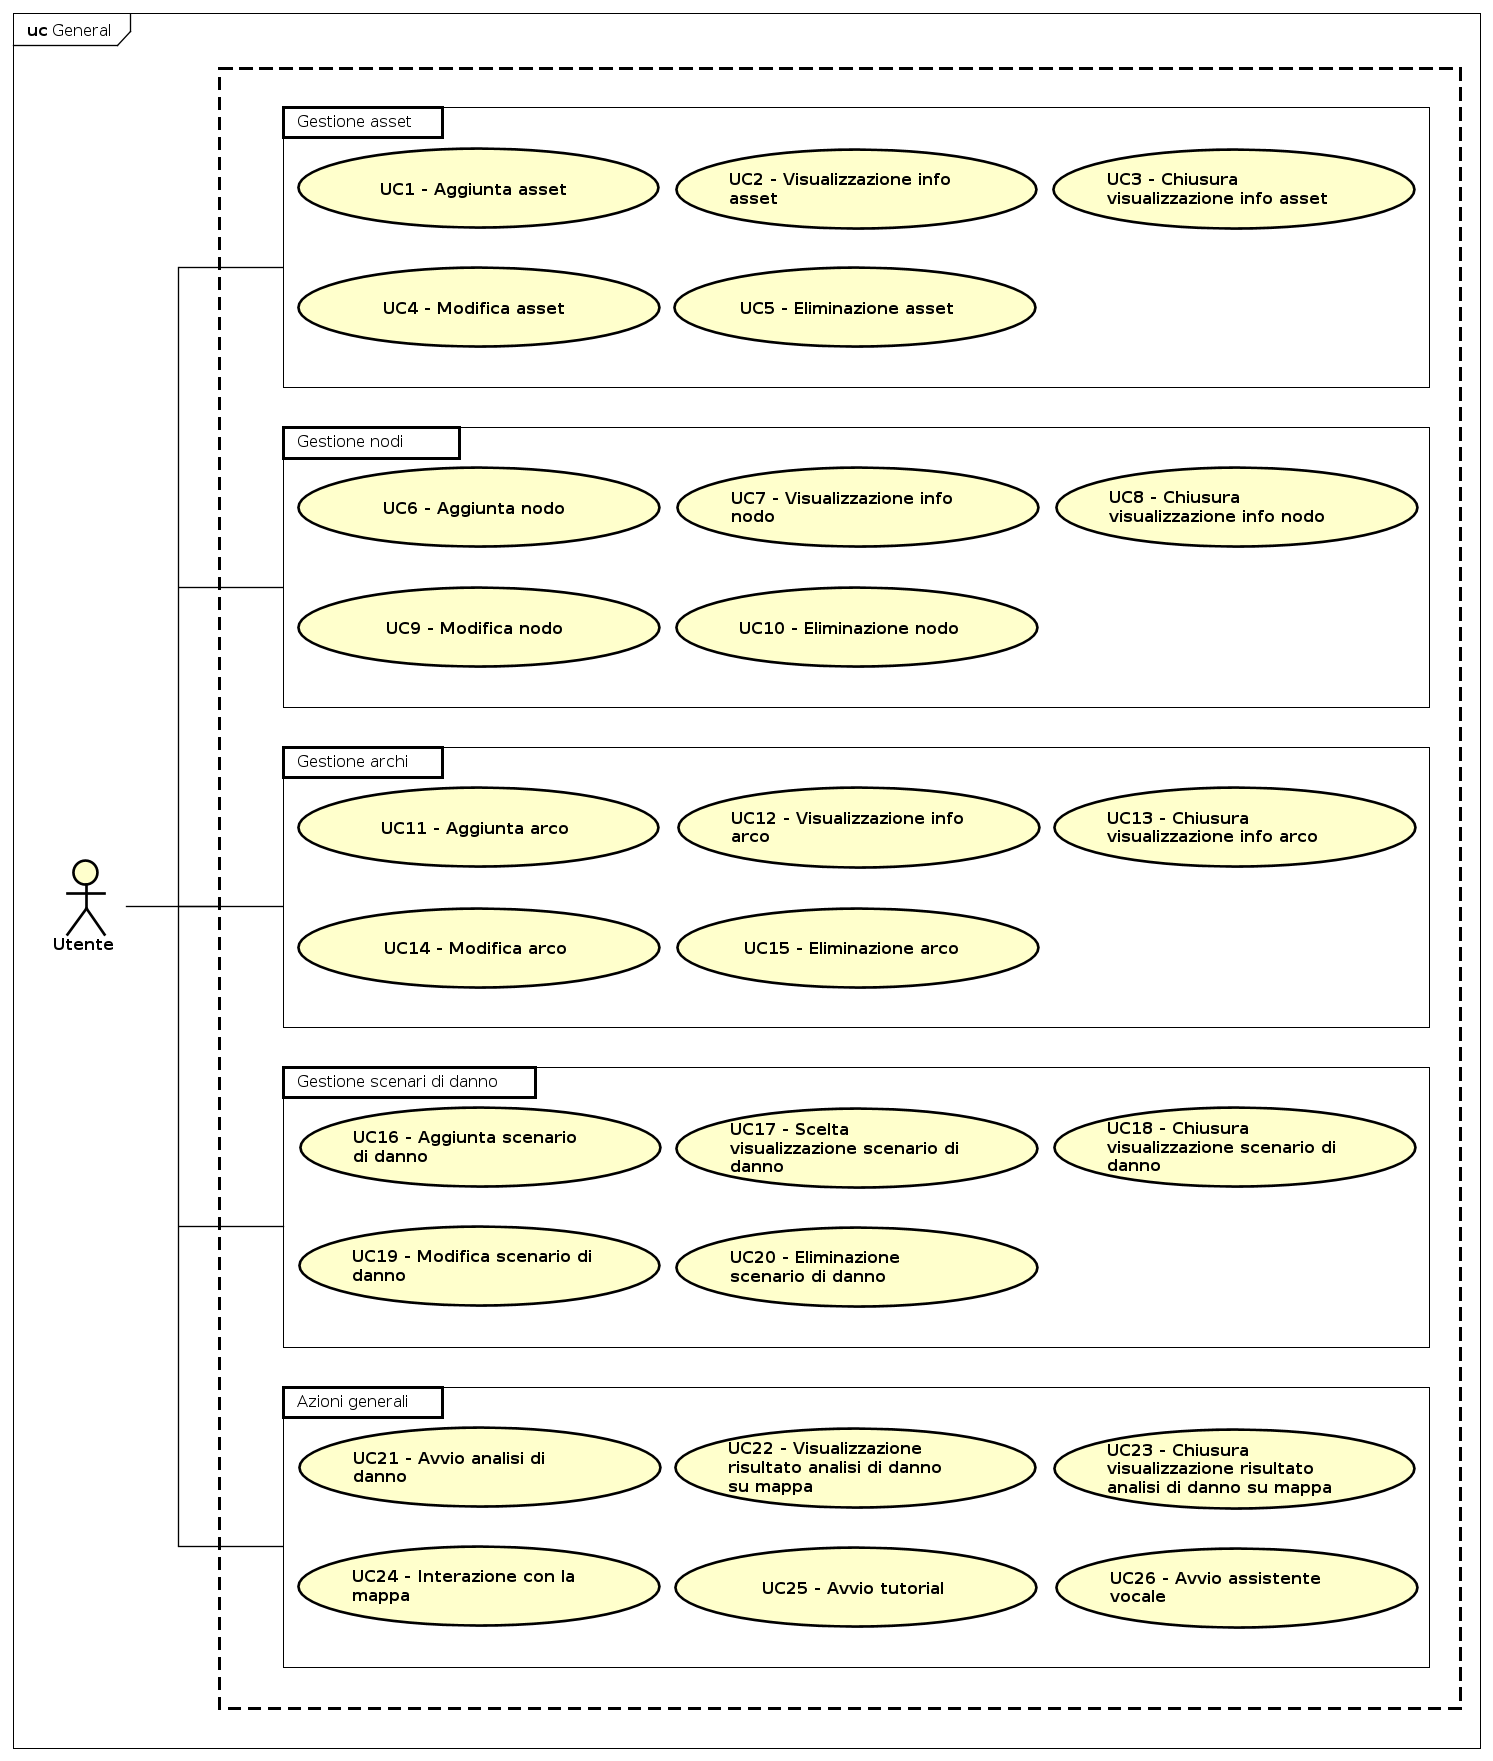
\includegraphics[width=\textwidth]{{img/uc0}.png}
\caption{Panoramica generale dei casi d'uso}
\end{figure}
\subsection{UC1 - Aggiunta asset}
\label{sssec:UC1}
\begin{figure}[H]
\centering
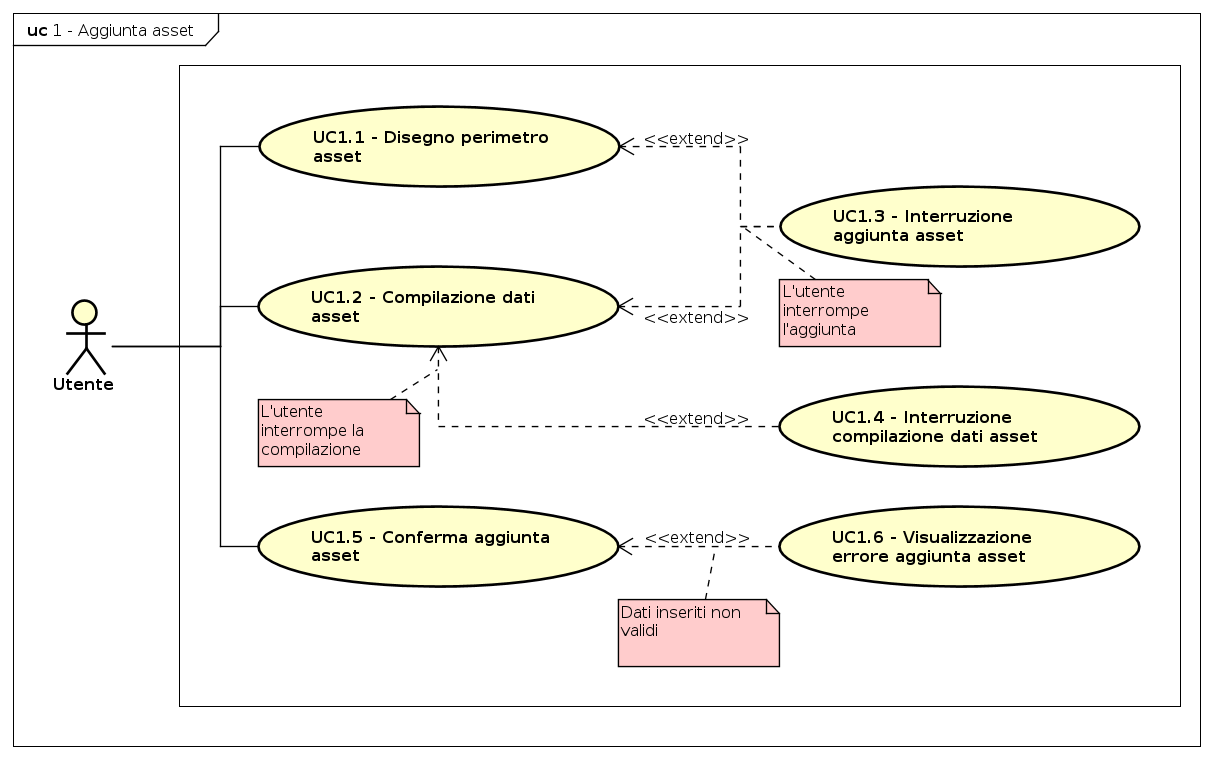
\includegraphics[width=\textwidth]{{img/uc1}.png}
\caption{UC1 - Aggiunta asset}
\end{figure}
\def\arraystretch{1.5}
\rowcolors{2}{D}{P}
\begin{tabularx}{\textwidth}{l|p{0.7\textwidth}}
\rowcolor{I} \multicolumn{2}{c}{\color{white}\textbf{UC1 - Aggiunta asset}} \\
\toprule
\endhead
\textbf{Attori} & Utente\\
\textbf{Descrizione} & l'utente aggiunge un asset\\
\textbf{Pre-condizione} & l'utente ha aperto l'applicazione\\
\textbf{Post-condizione} & un nuovo asset è stato aggiunto\\
\textbf{Scenario principale} & \vspace{-1.2em}\begin{enumerate}[leftmargin=*,noitemsep,nosep]
\item \nameref{sssec:UC1.1};
\item \nameref{sssec:UC1.2};
\item \nameref{sssec:UC1.5}.
\end{enumerate}\\
\textbf{Scenari alternativi} & \vspace{-1.2em}\begin{itemize}[leftmargin=*,noitemsep,nosep]
\item \nameref{sssec:UC1.3};
\item \nameref{sssec:UC1.4};
\item \nameref{sssec:UC1.6}.
\end{itemize}\\
%\textbf{Generalizzazioni} &  \\
\bottomrule
\end{tabularx}
\subsection{UC1.1 - Disegno perimetro asset}
\label{sssec:UC1.1}
\begin{figure}[H]
\centering
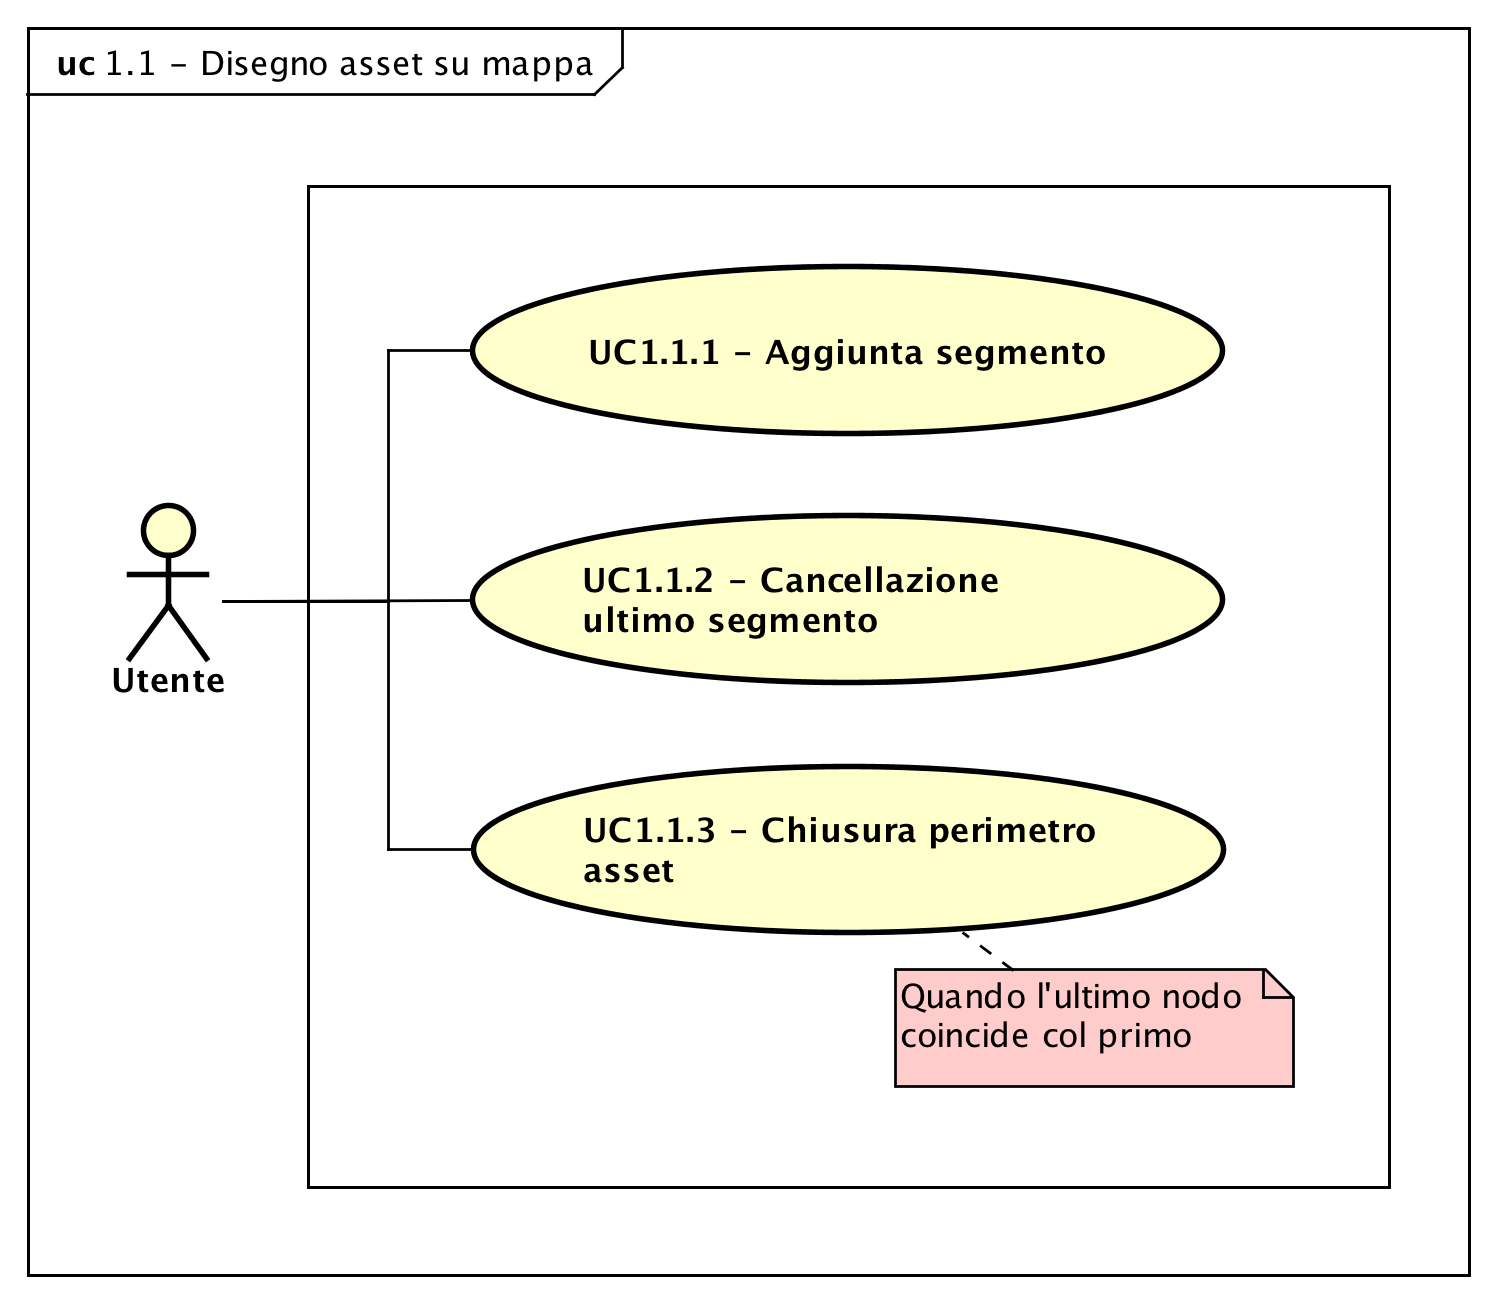
\includegraphics[scale=0.5]{{img/uc1.1}.png}
\caption{UC1.1 - Disegno perimetro asset}
\end{figure}
\def\arraystretch{1.5}
\rowcolors{2}{D}{P}
\begin{tabularx}{\textwidth}{l|p{0.7\textwidth}}
\rowcolor{I} \multicolumn{2}{c}{\color{white}\textbf{UC1.1 - Disegno perimetro asset}} \\
\toprule
\endhead
\textbf{Attori} & Utente\\
\textbf{Descrizione} & l'utente disegna su mappa il perimetro dell'asset\\
\textbf{Pre-condizione} & il sistema offre la possibilità disegnare su mappa il perimetro dell'asset\\
\textbf{Post-condizione} & il perimetro dell'asset è stato disegnato\\
\textbf{Scenario principale} & \vspace{-1.2em}\begin{enumerate}[leftmargin=*,noitemsep,nosep]
\item \nameref{sssec:UC1.1.2};
\item \nameref{sssec:UC1.1.3}.
\end{enumerate}\\
\textbf{Estensioni} & \vspace{-1.2em}\begin{itemize}[leftmargin=*,noitemsep,nosep]
\item \nameref{sssec:UC1.3}.
\end{itemize}\\
\textbf{Scenari alternativi} & \vspace{-1.2em}\begin{itemize}[leftmargin=*,noitemsep,nosep]
\item \nameref{sssec:UC1.1.1}.
\end{itemize}\\
%\textbf{Generalizzazioni} &  \\
\bottomrule
\end{tabularx}
\subsection{UC1.1.1 - Aggiunta segmento}
\label{sssec:UC1.1.1}
\def\arraystretch{1.5}
\rowcolors{2}{D}{P}
\begin{tabularx}{\textwidth}{l|p{0.7\textwidth}}
\rowcolor{I} \multicolumn{2}{c}{\color{white}\textbf{UC1.1.1 - Aggiunta segmento}} \\
\toprule
\endhead
\textbf{Attori} & Utente\\
\textbf{Descrizione} & l'utente aggiunge un segmento al perimetro dell'asset che sta disegnando\\
\textbf{Pre-condizione} & il sistema offre la possibilità di aggiungere un segmento al perimetro dell'asset\\
\textbf{Post-condizione} & l'utente ha aggiunto un segmento al perimetro dell'asset che sta disegnando\\
%\textbf{Generalizzazioni} &  \\
\bottomrule
\end{tabularx}
\subsection{UC1.1.2 - Cancellazione ultimo segmento}
\label{sssec:UC1.1.2}
\def\arraystretch{1.5}
\rowcolors{2}{D}{P}
\begin{tabularx}{\textwidth}{l|p{0.7\textwidth}}
\rowcolor{I} \multicolumn{2}{c}{\color{white}\textbf{UC1.1.2 - Cancellazione ultimo segmento}} \\
\toprule
\endhead
\textbf{Attori} & Utente\\
\textbf{Descrizione} & l'utente cancella l'ultimo segmento del perimetro dell'asset che sta disegnando\\
\textbf{Pre-condizione} & l'utente sta disegnando il perimetro di un asset; è stato disegnato almeno un segmento\\
\textbf{Post-condizione} & l'utente ha cancellato l'ultimo segmento del perimetro dell'asset che sta disegnando\\
%\textbf{Generalizzazioni} &  \\
\bottomrule
\end{tabularx}
\subsection{UC1.1.3 - Chiusura perimetro asset}
\label{sssec:UC1.1.3}
\def\arraystretch{1.5}
\rowcolors{2}{D}{P}
\begin{tabularx}{\textwidth}{l|p{0.7\textwidth}}
\rowcolor{I} \multicolumn{2}{c}{\color{white}\textbf{UC1.1.3 - Chiusura perimetro asset}} \\
\toprule
\endhead
\textbf{Attori} & Utente\\
\textbf{Descrizione} & l'utente termina di disegnare il perimetro di un asset, facendo coincidere ultimo e primo nodo\\
\textbf{Pre-condizione} & il sistema offre la possibilità  disegnare il perimetro di un asset; l'utente ha disegnato almeno due segmenti\\
\textbf{Post-condizione} & l'utente ha terminato di disegnare il perimetro di un asset\\
%\textbf{Generalizzazioni} &  \\
\bottomrule
\end{tabularx}
\subsection{UC1.2 - Compilazione dati asset}
\label{sssec:UC1.2}
\begin{figure}[H]
\centering
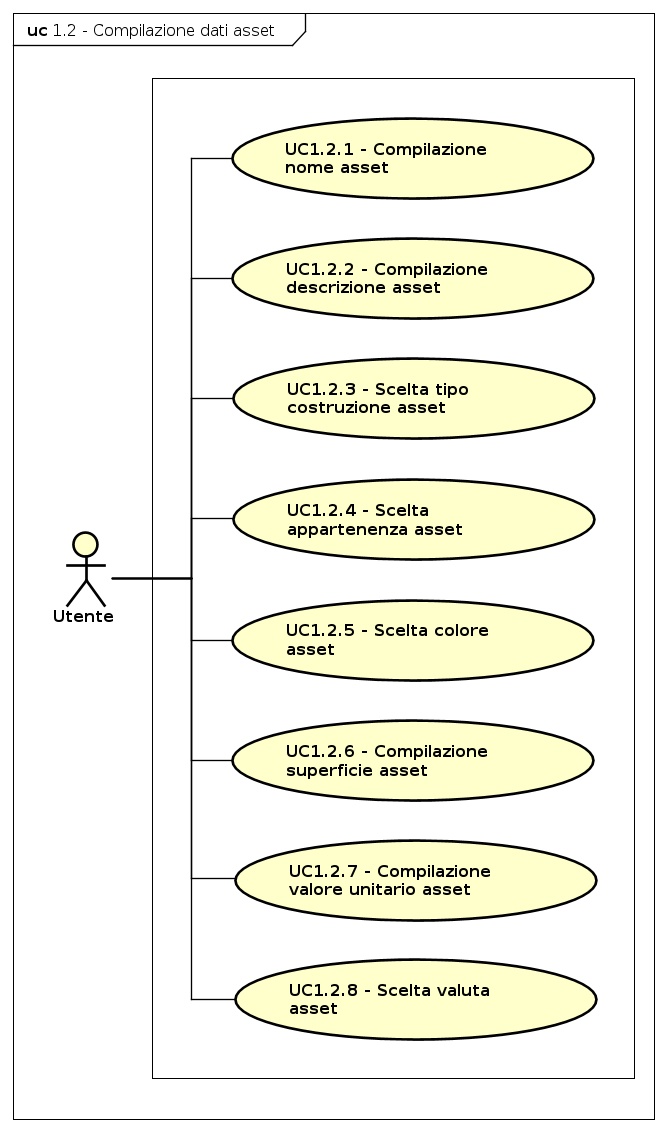
\includegraphics[scale=0.5]{{img/uc1.2}.png}
\caption{UC1.2 - Compilazione dati asset}
\end{figure}
\def\arraystretch{1.5}
\rowcolors{2}{D}{P}
\begin{tabularx}{\textwidth}{l|p{0.7\textwidth}}
\rowcolor{I} \multicolumn{2}{c}{\color{white}\textbf{UC1.2 - Compilazione dati asset}} \\
\toprule
\endhead
\textbf{Attori} & Utente\\
\textbf{Descrizione} & l'utente compila i dati dell'asset che sta aggiungendo\\
\textbf{Pre-condizione} & il sistema offre la possibilità di compilare i dati dell'asset\\
\textbf{Post-condizione} & l'utente ha compilato i dati dell'asset che sta aggiungendo\\
\textbf{Scenario principale} & \vspace{-1.2em}\begin{enumerate}[leftmargin=*,noitemsep,nosep]
\item \nameref{sssec:UC1.2.1};
\item \nameref{sssec:UC1.2.2};
\item \nameref{sssec:UC1.2.3};
\item \nameref{sssec:UC1.2.4};
\item \nameref{sssec:UC1.2.5};
\item \nameref{sssec:UC1.2.6};
\item \nameref{sssec:UC1.2.7};
\item \nameref{sssec:UC1.2.8}.
\end{enumerate}\\
\textbf{Estensioni} & \vspace{-1.2em}\begin{itemize}[leftmargin=*,noitemsep,nosep]
\item \nameref{sssec:UC1.3};

\item \nameref{sssec:UC1.4}.
\end{itemize}\\
%\textbf{Generalizzazioni} &  \\
\bottomrule
\end{tabularx}
\subsection{UC1.2.1 - Compilazione nome asset}
\label{sssec:UC1.2.1}
\def\arraystretch{1.5}
\rowcolors{2}{D}{P}
\begin{tabularx}{\textwidth}{l|p{0.7\textwidth}}
\rowcolor{I} \multicolumn{2}{c}{\color{white}\textbf{UC1.2.1 - Compilazione nome asset}} \\
\toprule
\endhead
\textbf{Attori} & Utente\\
\textbf{Descrizione} & l'utente compila il nome dell'asset\\
\textbf{Pre-condizione} & il sistema offre la possibilità di compilare il nome dell'asset\\
\textbf{Post-condizione} & l'utente ha compilato il nome dell'asset\\
%\textbf{Generalizzazioni} &  \\
\bottomrule
\end{tabularx}
\subsection{UC1.2.2 - Compilazione descrizione asset}
\label{sssec:UC1.2.2}
\def\arraystretch{1.5}
\rowcolors{2}{D}{P}
\begin{tabularx}{\textwidth}{l|p{0.7\textwidth}}
\rowcolor{I} \multicolumn{2}{c}{\color{white}\textbf{UC1.2.2 - Compilazione descrizione asset}} \\
\toprule
\endhead
\textbf{Attori} & Utente\\
\textbf{Descrizione} & l'utente compila la descrizione dell'asset\\
\textbf{Pre-condizione} & il sistema offre la possibilità di compilare la descrizione dell'asset\\
\textbf{Post-condizione} & l'utente ha compilato la descrizione dell'asset\\
%\textbf{Generalizzazioni} &  \\
\bottomrule
\end{tabularx}
\subsection{UC1.2.3 - Scelta tipo costruzione asset}
\label{sssec:UC1.2.3}
\def\arraystretch{1.5}
\rowcolors{2}{D}{P}
\begin{tabularx}{\textwidth}{l|p{0.7\textwidth}}
\rowcolor{I} \multicolumn{2}{c}{\color{white}\textbf{UC1.2.3 - Scelta tipo costruzione asset}} \\
\toprule
\endhead
\textbf{Attori} & Utente\\
\textbf{Descrizione} & l'utente sceglie il tipo di costruzione dell'asset\\
\textbf{Pre-condizione} & il sistema offre la possibilità di scegliere il tipo di costruzione dell'asset\\
\textbf{Post-condizione} & l'utente ha scelto il tipo di costruzione dell'asset\\
%\textbf{Generalizzazioni} &  \\
\bottomrule
\end{tabularx}
\subsection{UC1.2.4 - Scelta appartenenza asset}
\label{sssec:UC1.2.4}
\def\arraystretch{1.5}
\rowcolors{2}{D}{P}
\begin{tabularx}{\textwidth}{l|p{0.7\textwidth}}
\rowcolor{I} \multicolumn{2}{c}{\color{white}\textbf{UC1.2.4 - Scelta appartenenza asset}} \\
\toprule
\endhead
\textbf{Attori} & Utente\\
\textbf{Descrizione} & l'utente sceglie a chi appartiene l'asset\\
\textbf{Pre-condizione} & il sistema offre la possibilità di scegliere a chi appartiene l'asset\\
\textbf{Post-condizione} & l'utente ha scelto a chi appartiene l'asset\\
%\textbf{Generalizzazioni} &  \\
\bottomrule
\end{tabularx}
\subsection{UC1.2.5 - Scelta colore asset}
\label{sssec:UC1.2.5}
\def\arraystretch{1.5}
\rowcolors{2}{D}{P}
\begin{tabularx}{\textwidth}{l|p{0.7\textwidth}}
\rowcolor{I} \multicolumn{2}{c}{\color{white}\textbf{UC1.2.5 - Scelta colore asset}} \\
\toprule
\endhead
\textbf{Attori} & Utente\\
\textbf{Descrizione} & l'utente sceglie il colore dell'asset\\
\textbf{Pre-condizione} & il sistema offre la possibilità di scegliere il colore dell'asset\\
\textbf{Post-condizione} & l'utente ha scelto il colore dell'asset\\
%\textbf{Generalizzazioni} &  \\
\bottomrule
\end{tabularx}
\subsection{UC1.2.6 - Compilazione superficie asset}
\label{sssec:UC1.2.6}
\def\arraystretch{1.5}
\rowcolors{2}{D}{P}
\begin{tabularx}{\textwidth}{l|p{0.7\textwidth}}
\rowcolor{I} \multicolumn{2}{c}{\color{white}\textbf{UC1.2.6 - Compilazione superficie asset}} \\
\toprule
\endhead
\textbf{Attori} & Utente\\
\textbf{Descrizione} & l'utente compila la superficie dell'asset\\
\textbf{Pre-condizione} & il sistema offre la possibilità di compilare la superficie dell'asset\\
\textbf{Post-condizione} & l'utente ha compilato la superficie dell'asset\\
%\textbf{Generalizzazioni} &  \\
\bottomrule
\end{tabularx}
\subsection{UC1.2.7 - Compilazione valore unitario asset}
\label{sssec:UC1.2.7}
\def\arraystretch{1.5}
\rowcolors{2}{D}{P}
\begin{tabularx}{\textwidth}{l|p{0.7\textwidth}}
\rowcolor{I} \multicolumn{2}{c}{\color{white}\textbf{UC1.2.7 - Compilazione valore unitario asset}} \\
\toprule
\endhead
\textbf{Attori} & Utente\\
\textbf{Descrizione} & l'utente compila il valore unitario dell'asset\\
\textbf{Pre-condizione} & il sistema offre la possibilità di compilare il valore unitario dell'asset\\
\textbf{Post-condizione} & l'utente ha compilato il valore unitario dell'asset\\
%\textbf{Generalizzazioni} &  \\
\bottomrule
\end{tabularx}
\subsection{UC1.2.8 - Scelta valuta asset}
\label{sssec:UC1.2.8}
\def\arraystretch{1.5}
\rowcolors{2}{D}{P}
\begin{tabularx}{\textwidth}{l|p{0.7\textwidth}}
\rowcolor{I} \multicolumn{2}{c}{\color{white}\textbf{UC1.2.8 - Scelta valuta asset}} \\
\toprule
\endhead
\textbf{Attori} & Utente\\
\textbf{Descrizione} & l'utente sceglie la valuta del valore unitario dell'asset\\
\textbf{Pre-condizione} & il sistema offre la possibilità di scegliere la valuta del valore unitario dell'asset\\
\textbf{Post-condizione} & l'utente ha scelto la valuta del valore unitario dell'asset\\
%\textbf{Generalizzazioni} &  \\
\bottomrule
\end{tabularx}
\subsection{UC1.3 - Interruzione aggiunta asset}
\label{sssec:UC1.3}
\def\arraystretch{1.5}
\rowcolors{2}{D}{P}
\begin{tabularx}{\textwidth}{l|p{0.7\textwidth}}
\rowcolor{I} \multicolumn{2}{c}{\color{white}\textbf{UC1.3 - Interruzione aggiunta asset}} \\
\toprule
\endhead
\textbf{Attori} & Utente\\
\textbf{Descrizione} & l'utente interrompe l'aggiunta dell'asset\\
\textbf{Pre-condizione} & il sistema offre la possibilità di aggiungere un asset\\
\textbf{Post-condizione} & nessun asset è stato aggiunto\\
%\textbf{Generalizzazioni} &  \\
\bottomrule
\end{tabularx}
\subsection{UC1.4 - Interruzione compilazione dati asset}
\label{sssec:UC1.4}
\def\arraystretch{1.5}
\rowcolors{2}{D}{P}
\begin{tabularx}{\textwidth}{l|p{0.7\textwidth}}
\rowcolor{I} \multicolumn{2}{c}{\color{white}\textbf{UC1.4 - Interruzione compilazione dati asset}} \\
\toprule
\endhead
\textbf{Attori} & Utente\\
\textbf{Descrizione} & l'utente interrompe la compilazione dei dati dell'asset\\
\textbf{Pre-condizione} & il sistema offre la possibilità di compilare i dati dell'asset\\
\textbf{Post-condizione} & i dati dell'asset non sono stati compilati; l'utente viene riportato alla fase di disegno dell'asset\\
%\textbf{Generalizzazioni} &  \\
\bottomrule
\end{tabularx}
\subsection{UC1.5 - Conferma aggiunta asset}
\label{sssec:UC1.5}
\def\arraystretch{1.5}
\rowcolors{2}{D}{P}
\begin{tabularx}{\textwidth}{l|p{0.7\textwidth}}
\rowcolor{I} \multicolumn{2}{c}{\color{white}\textbf{UC1.5 - Conferma aggiunta asset}} \\
\toprule
\endhead
\textbf{Attori} & Utente\\
\textbf{Descrizione} & l'utente conferma l'aggiunta dell'asset\\
\textbf{Pre-condizione} & il sistema offre la possibilità di confermare l'aggiunta dell'asset\\
\textbf{Post-condizione} & un nuovo asset è stato aggiunto\\
\textbf{Estensioni} & \vspace{-1.2em}\begin{itemize}[leftmargin=*,noitemsep,nosep]
\item \nameref{sssec:UC1.6}.
\end{itemize}\\
%\textbf{Generalizzazioni} &  \\
\bottomrule
\end{tabularx}
\subsection{UC1.6 - Visualizzazione errore aggiunta asset}
\label{sssec:UC1.6}
\def\arraystretch{1.5}
\rowcolors{2}{D}{P}
\begin{tabularx}{\textwidth}{l|p{0.7\textwidth}}
\rowcolor{I} \multicolumn{2}{c}{\color{white}\textbf{UC1.6 - Visualizzazione errore aggiunta asset}} \\
\toprule
\endhead
\textbf{Attori} & Utente\\
\textbf{Descrizione} & l'utente visualizza un errore relativo ai dati dell'asset compilati in modo errato\\
\textbf{Pre-condizione} & l'utente sta tentando di inserire un nuovo asset\\
\textbf{Post-condizione} & nessun nuovo asset inserito; l'utente visualizza un errore relativo ai dati dell'asset compilati in modo errato\\
%\textbf{Generalizzazioni} &  \\
\bottomrule
\end{tabularx}
\subsection{UC3 - Chiusura visualizzazione info asset}
\label{sssec:UC3}
\def\arraystretch{1.5}
\rowcolors{2}{D}{P}
\begin{tabularx}{\textwidth}{l|p{0.7\textwidth}}
\rowcolor{I} \multicolumn{2}{c}{\color{white}\textbf{UC3 - Chiusura visualizzazione info asset}} \\
\toprule
\endhead
\textbf{Attori} & Utente\\
\textbf{Descrizione} & l'utente chiude la visualizzazione delle informazioni di un asset\\
\textbf{Pre-condizione} & l'utente ha visualizzato le informazioni di un asset\\
\textbf{Post-condizione} & è stata chiusa la visualizzazione delle informazioni di un asset\\
%\textbf{Generalizzazioni} &  \\
\bottomrule
\end{tabularx}
\subsection{UC4 - Modifica asset}
\label{sssec:UC4}
\begin{figure}[H]
\centering
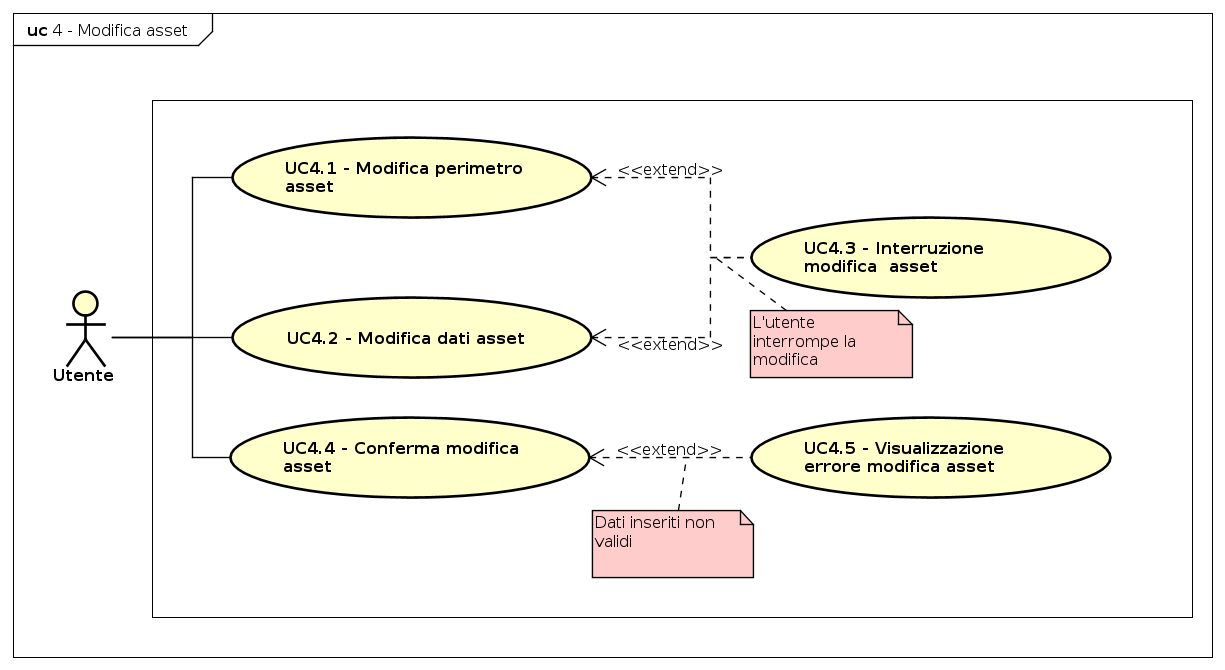
\includegraphics[width=\textwidth]{{img/uc4}.png}
\caption{UC4 - Modifica asset}
\end{figure}
\def\arraystretch{1.5}
\rowcolors{2}{D}{P}
\begin{tabularx}{\textwidth}{l|p{0.7\textwidth}}
\rowcolor{I} \multicolumn{2}{c}{\color{white}\textbf{UC4 - Modifica asset}} \\
\toprule
\endhead
\textbf{Attori} & Utente\\
\textbf{Descrizione} & l'utente modifica l'asset\\
\textbf{Pre-condizione} & l'utente ha aperto l'applicazione; almeno un asset è stato aggiunto; l'utente ha selezionato un asset\\
\textbf{Post-condizione} & l'asset è stato modificato\\
\textbf{Scenario principale} & \vspace{-1.2em}\begin{enumerate}[leftmargin=*,noitemsep,nosep]
\item \nameref{sssec:UC4.1};
\item \nameref{sssec:UC4.2};
\item \nameref{sssec:UC4.4}.
\end{enumerate}\\
\textbf{Scenari alternativi} & \vspace{-1.2em}\begin{itemize}[leftmargin=*,noitemsep,nosep]
\item \nameref{sssec:UC4.3};
\item \nameref{sssec:UC4.5}.
\end{itemize}\\
%\textbf{Generalizzazioni} &  \\
\bottomrule
\end{tabularx}
\subsection{UC4.1 - Modifica perimetro asset}
\label{sssec:UC4.1}
\begin{figure}[H]
\centering
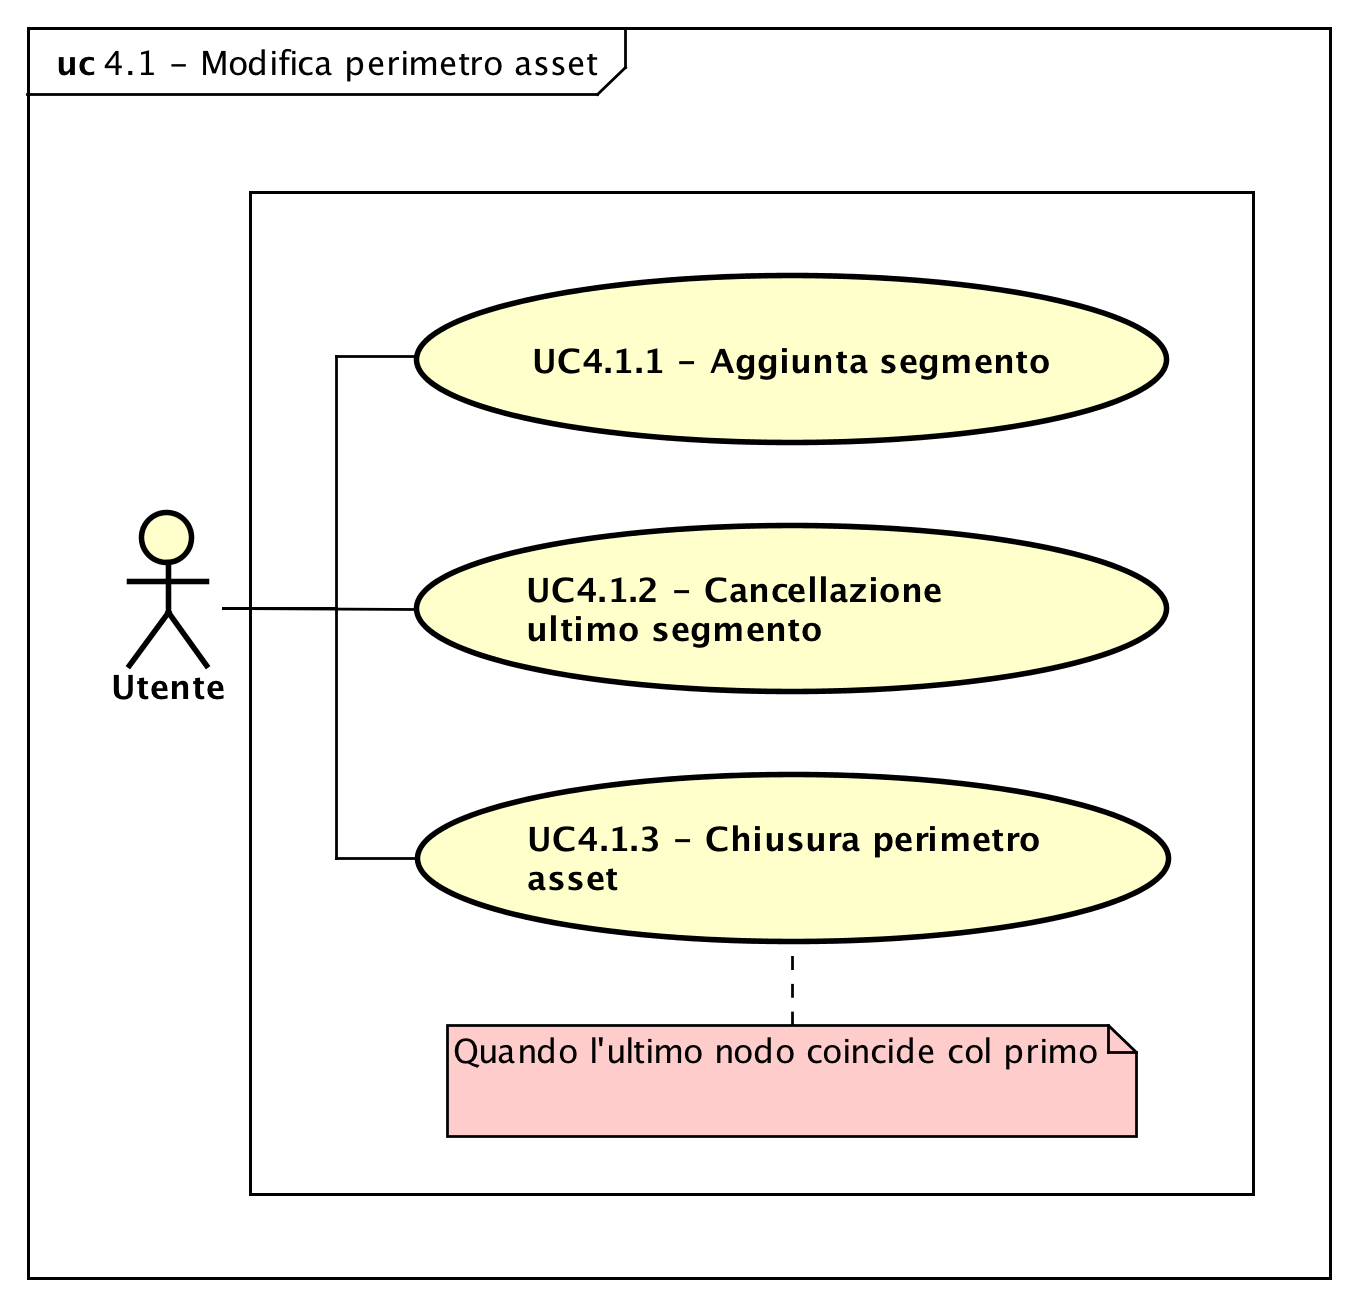
\includegraphics[scale=0.5]{{img/uc4.1}.png}
\caption{UC4.1 - Modifica perimetro asset}
\end{figure}
\def\arraystretch{1.5}
\rowcolors{2}{D}{P}
\begin{tabularx}{\textwidth}{l|p{0.7\textwidth}}
\rowcolor{I} \multicolumn{2}{c}{\color{white}\textbf{UC4.1 - Modifica perimetro asset}} \\
\toprule
\endhead
\textbf{Attori} & Utente\\
\textbf{Descrizione} & l'utente modifica il perimetro dell'asset\\
\textbf{Pre-condizione} & il sistema offre la possibilità di modificare il perimetro dell'asset\\
\textbf{Post-condizione} & il perimetro dell'asset è stato modificato\\
\textbf{Scenario principale} & \vspace{-1.2em}\begin{enumerate}[leftmargin=*,noitemsep,nosep]
\item \nameref{sssec:UC4.1.1};
\item \nameref{sssec:UC4.1.2};
\item \nameref{sssec:UC4.1.3}.
\end{enumerate}\\
\textbf{Estensioni} & \vspace{-1.2em}\begin{itemize}[leftmargin=*,noitemsep,nosep]
\item \nameref{sssec:UC4.3}.
\end{itemize}\\
%\textbf{Generalizzazioni} &  \\
\bottomrule
\end{tabularx}
\subsection{UC4.1.1 - Aggiunta segmento}
\label{sssec:UC4.1.1}
\def\arraystretch{1.5}
\rowcolors{2}{D}{P}
\begin{tabularx}{\textwidth}{l|p{0.7\textwidth}}
\rowcolor{I} \multicolumn{2}{c}{\color{white}\textbf{UC4.1.1 - Aggiunta segmento}} \\
\toprule
\endhead
\textbf{Attori} & Utente\\
\textbf{Descrizione} & l'utente aggiunge un segmento al perimetro dell'asset che sta modificando\\
\textbf{Pre-condizione} & il sistema offre la possibilità di aggiungere un segmento al perimetro dell'asset\\
\textbf{Post-condizione} & l'utente ha aggiunto un segmento al perimetro dell'asset che sta modificando\\
%\textbf{Generalizzazioni} &  \\
\bottomrule
\end{tabularx}
\subsection{UC4.1.2 - Cancellazione ultimo segmento}
\label{sssec:UC4.1.2}
\def\arraystretch{1.5}
\rowcolors{2}{D}{P}
\begin{tabularx}{\textwidth}{l|p{0.7\textwidth}}
\rowcolor{I} \multicolumn{2}{c}{\color{white}\textbf{UC4.1.2 - Cancellazione ultimo segmento}} \\
\toprule
\endhead
\textbf{Attori} & Utente\\
\textbf{Descrizione} & l'utente cancella l'ultimo segmento del perimetro dell'asset che sta modificando\\
\textbf{Pre-condizione} & l'utente sta disegnando il perimetro di un asset; è stato disegnato almeno un segmento\\
\textbf{Post-condizione} & l'utente ha cancellato l'ultimo segmento del perimetro dell'asset che sta modificando\\
%\textbf{Generalizzazioni} &  \\
\bottomrule
\end{tabularx}
\subsection{UC4.1.3 - Chiusura perimetro asset}
\label{sssec:UC4.1.3}
\def\arraystretch{1.5}
\rowcolors{2}{D}{P}
\begin{tabularx}{\textwidth}{l|p{0.7\textwidth}}
\rowcolor{I} \multicolumn{2}{c}{\color{white}\textbf{UC4.1.3 - Chiusura perimetro asset}} \\
\toprule
\endhead
\textbf{Attori} & Utente\\
\textbf{Descrizione} & l'utente termina di disegnare il perimetro dell'asset che sta modificando, facendo coincidere ultimo e primo nodo\\
\textbf{Pre-condizione} & il sistema offre la possibilità  disegnare il perimetro dell'asset; l'utente ha disegnato almeno due segmenti\\
\textbf{Post-condizione} & l'utente ha terminato di disegnare il perimetro di un asset\\
%\textbf{Generalizzazioni} &  \\
\bottomrule
\end{tabularx}
\subsection{UC4.2 - Modifica dati asset}
\label{sssec:UC4.2}
\begin{figure}[H]
\centering
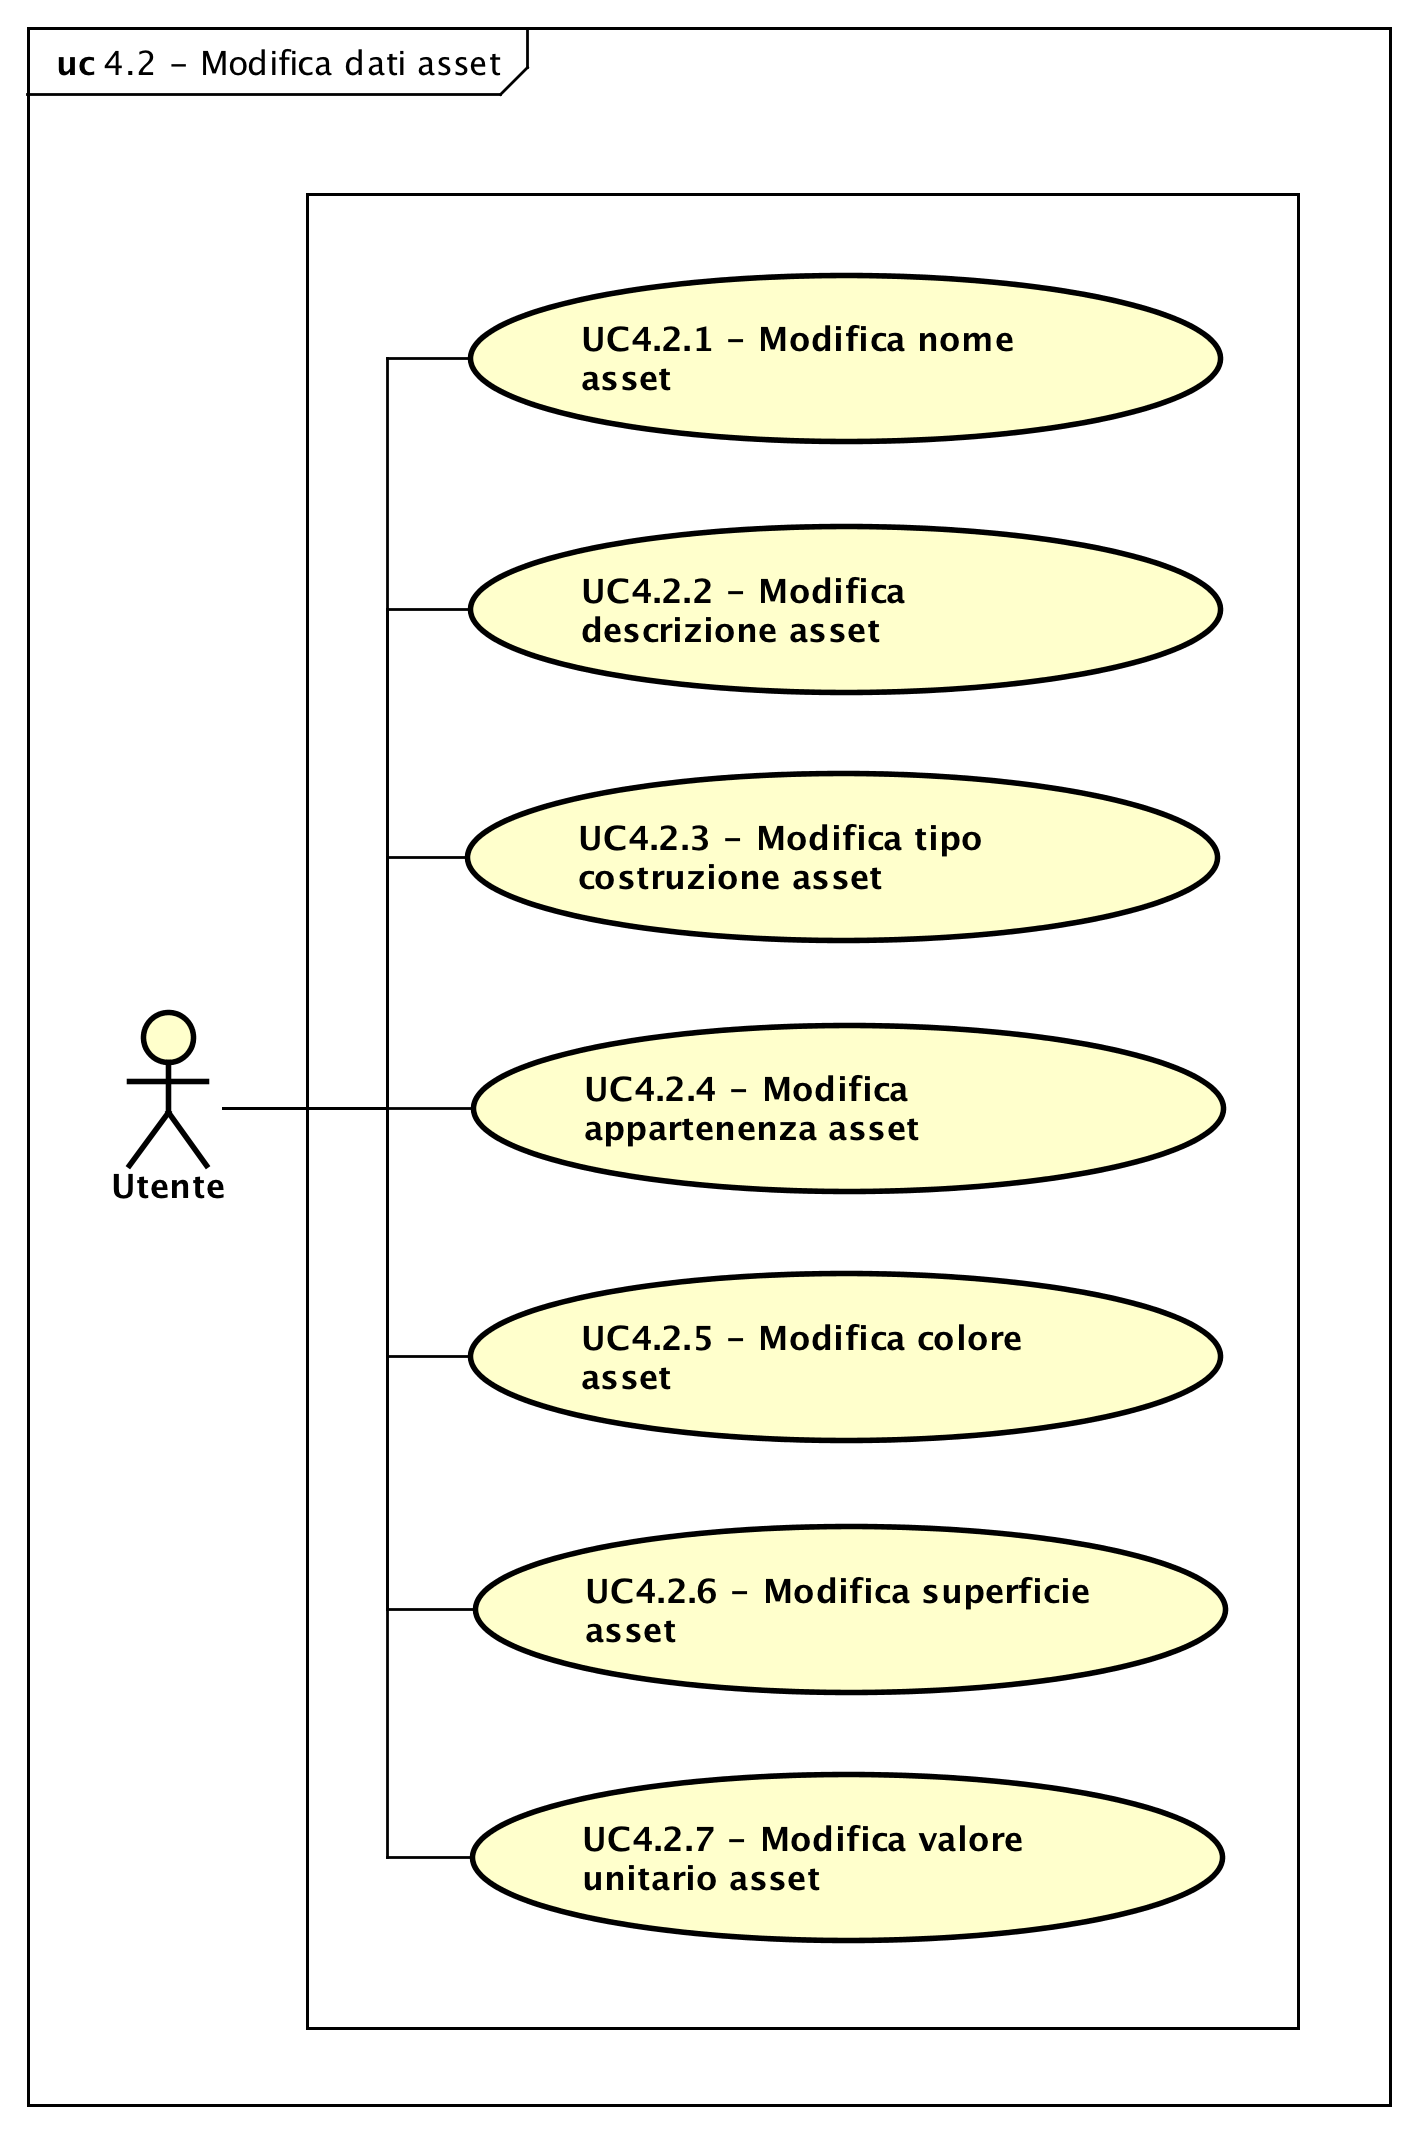
\includegraphics[scale=0.5]{{img/uc4.2}.png}
\caption{UC4.2 - Modifica dati asset}
\end{figure}
\def\arraystretch{1.5}
\rowcolors{2}{D}{P}
\begin{tabularx}{\textwidth}{l|p{0.7\textwidth}}
\rowcolor{I} \multicolumn{2}{c}{\color{white}\textbf{UC4.2 - Modifica dati asset}} \\
\toprule
\endhead
\textbf{Attori} & Utente\\
\textbf{Descrizione} & l'utente modifica i dati dell'asset\\
\textbf{Pre-condizione} & il sistema offre la possibilità di modificare i dati dell'asset\\
\textbf{Post-condizione} & i dati dell'asset sono stati modificati\\
\textbf{Scenario principale} & \vspace{-1.2em}\begin{enumerate}[leftmargin=*,noitemsep,nosep]
\item \nameref{sssec:UC4.2.1};
\item \nameref{sssec:UC4.2.2};
\item \nameref{sssec:UC4.2.3};
\item \nameref{sssec:UC4.2.4};
\item \nameref{sssec:UC4.2.5};
\item \nameref{sssec:UC4.2.6};
\item \nameref{sssec:UC4.2.7};
\item \nameref{sssec:UC4.2.8}.
\end{enumerate}\\
\textbf{Estensioni} & \vspace{-1.2em}\begin{itemize}[leftmargin=*,noitemsep,nosep]
\item \nameref{sssec:UC4.3}.
\end{itemize}\\
%\textbf{Generalizzazioni} &  \\
\bottomrule
\end{tabularx}
\subsection{UC4.2.1 - Modifica nome asset}
\label{sssec:UC4.2.1}
\def\arraystretch{1.5}
\rowcolors{2}{D}{P}
\begin{tabularx}{\textwidth}{l|p{0.7\textwidth}}
\rowcolor{I} \multicolumn{2}{c}{\color{white}\textbf{UC4.2.1 - Modifica nome asset}} \\
\toprule
\endhead
\textbf{Attori} & Utente\\
\textbf{Descrizione} & l'utente modifica il campo relativo al nome dell'asset\\
\textbf{Pre-condizione} & il sistema offre la possibilità di modificare il nome dell'asset\\
\textbf{Post-condizione} & il campo relativo al nome dell'asset è stato modificato\\
%\textbf{Generalizzazioni} &  \\
\bottomrule
\end{tabularx}
\subsection{UC4.2.2 - Modifica descrizione asset}
\label{sssec:UC4.2.2}
\def\arraystretch{1.5}
\rowcolors{2}{D}{P}
\begin{tabularx}{\textwidth}{l|p{0.7\textwidth}}
\rowcolor{I} \multicolumn{2}{c}{\color{white}\textbf{UC4.2.2 - Modifica descrizione asset}} \\
\toprule
\endhead
\textbf{Attori} & Utente\\
\textbf{Descrizione} & l'utente modifica il campo relativo alla descrizione dell'asset\\
\textbf{Pre-condizione} & il sistema offre la possibilità di modificare la descrizione dell'asset\\
\textbf{Post-condizione} & il campo relativo alla descrizione dell'asset è stato modificato\\
%\textbf{Generalizzazioni} &  \\
\bottomrule
\end{tabularx}
\subsection{UC4.2.3 - Modifica tipo costruzione asset}
\label{sssec:UC4.2.3}
\def\arraystretch{1.5}
\rowcolors{2}{D}{P}
\begin{tabularx}{\textwidth}{l|p{0.7\textwidth}}
\rowcolor{I} \multicolumn{2}{c}{\color{white}\textbf{UC4.2.3 - Modifica tipo costruzione asset}} \\
\toprule
\endhead
\textbf{Attori} & Utente\\
\textbf{Descrizione} & l'utente modifica la scelta relativa al tipo di costruzione dell'asset\\
\textbf{Pre-condizione} & il sistema offre la possibilità di modificare il tipo di costruzione dell'asset\\
\textbf{Post-condizione} & la scelta relativa al tipo di costruzione dell'asset è stata modificata\\
%\textbf{Generalizzazioni} &  \\
\bottomrule
\end{tabularx}
\subsection{UC4.2.4 - Modifica appartenenza asset}
\label{sssec:UC4.2.4}
\def\arraystretch{1.5}
\rowcolors{2}{D}{P}
\begin{tabularx}{\textwidth}{l|p{0.7\textwidth}}
\rowcolor{I} \multicolumn{2}{c}{\color{white}\textbf{UC4.2.4 - Modifica appartenenza asset}} \\
\toprule
\endhead
\textbf{Attori} & Utente\\
\textbf{Descrizione} & l'utente modifica la scelta relativa al proprietario dell'asset\\
\textbf{Pre-condizione} & il sistema offre la possibilità di modificare l'appartenenza dell'asset\\
\textbf{Post-condizione} & la scelta relativa la proprietario dell'asset è stata modificata\\
%\textbf{Generalizzazioni} &  \\
\bottomrule
\end{tabularx}
\subsection{UC4.2.5 - Modifica colore asset}
\label{sssec:UC4.2.5}
\def\arraystretch{1.5}
\rowcolors{2}{D}{P}
\begin{tabularx}{\textwidth}{l|p{0.7\textwidth}}
\rowcolor{I} \multicolumn{2}{c}{\color{white}\textbf{UC4.2.5 - Modifica colore asset}} \\
\toprule
\endhead
\textbf{Attori} & Utente\\
\textbf{Descrizione} & l'utente modifica la scelta relativa al colore dell'asset\\
\textbf{Pre-condizione} & il sistema offre la possibilità di modificare il colore dell'asset\\
\textbf{Post-condizione} & la scelta relativa al colore dell'asset è stata modificata\\
%\textbf{Generalizzazioni} &  \\
\bottomrule
\end{tabularx}
\subsection{UC4.2.6 - Modifica superficie asset}
\label{sssec:UC4.2.6}
\def\arraystretch{1.5}
\rowcolors{2}{D}{P}
\begin{tabularx}{\textwidth}{l|p{0.7\textwidth}}
\rowcolor{I} \multicolumn{2}{c}{\color{white}\textbf{UC4.2.6 - Modifica superficie asset}} \\
\toprule
\endhead
\textbf{Attori} & Utente\\
\textbf{Descrizione} & l'utente modifica il campo relativo alla superficie dell'asset\\
\textbf{Pre-condizione} & il sistema offre la possibilità di modificare la superficie dell'asset\\
\textbf{Post-condizione} & il campo relativo alla superficie dell'asset è stato modificato\\
%\textbf{Generalizzazioni} &  \\
\bottomrule
\end{tabularx}
\subsection{UC4.2.7 - Modifica valore unitario asset}
\label{sssec:UC4.2.7}
\def\arraystretch{1.5}
\rowcolors{2}{D}{P}
\begin{tabularx}{\textwidth}{l|p{0.7\textwidth}}
\rowcolor{I} \multicolumn{2}{c}{\color{white}\textbf{UC4.2.7 - Modifica valore unitario asset}} \\
\toprule
\endhead
\textbf{Attori} & Utente\\
\textbf{Descrizione} & l'utente modifica il campo relativo al valore unitario dell'asset\\
\textbf{Pre-condizione} & il sistema offre la possibilità di modificare il valore unitario dell'asset\\
\textbf{Post-condizione} & il campo relativo al valore unitario dell'asset è stato modificato\\
%\textbf{Generalizzazioni} &  \\
\bottomrule
\end{tabularx}
\subsection{UC4.2.8 - Modifica valuta asset}
\label{sssec:UC4.2.8}
\def\arraystretch{1.5}
\rowcolors{2}{D}{P}
\begin{tabularx}{\textwidth}{l|p{0.7\textwidth}}
\rowcolor{I} \multicolumn{2}{c}{\color{white}\textbf{UC4.2.8 - Modifica valuta asset}} \\
\toprule
\endhead
\textbf{Attori} & Utente\\
\textbf{Descrizione} & l'utente modifica il campo relativo alla valuta dell'asset\\
\textbf{Pre-condizione} & il sistema offre la possibilità di modificare la valuta dell'asset\\
\textbf{Post-condizione} & il campo relativo alla valuta dell'asset è stato modificato\\
%\textbf{Generalizzazioni} &  \\
\bottomrule
\end{tabularx}
\subsection{UC4.3 - Interruzione modifica asset}
\label{sssec:UC4.3}
\def\arraystretch{1.5}
\rowcolors{2}{D}{P}
\begin{tabularx}{\textwidth}{l|p{0.7\textwidth}}
\rowcolor{I} \multicolumn{2}{c}{\color{white}\textbf{UC4.3 - Interruzione modifica asset}} \\
\toprule
\endhead
\textbf{Attori} & Utente\\
\textbf{Descrizione} & l'utente interrompe la modifica dell'asset\\
\textbf{Pre-condizione} & il sistema offre la possibilità di modificare un asset\\
\textbf{Post-condizione} & l'asset non è stato modificato\\
%\textbf{Generalizzazioni} &  \\
\bottomrule
\end{tabularx}
\subsection{UC4.4 - Conferma modifica asset}
\label{sssec:UC4.4}
\def\arraystretch{1.5}
\rowcolors{2}{D}{P}
\begin{tabularx}{\textwidth}{l|p{0.7\textwidth}}
\rowcolor{I} \multicolumn{2}{c}{\color{white}\textbf{UC4.4 - Conferma modifica asset}} \\
\toprule
\endhead
\textbf{Attori} & Utente\\
\textbf{Descrizione} & l'utente conferma la modifica dell'asset\\
\textbf{Pre-condizione} & il sistema offre la possibilità di confermare la modifica dell'asset\\
\textbf{Post-condizione} & l'asset è stato modificato\\
\textbf{Estensioni} & \vspace{-1.2em}\begin{itemize}[leftmargin=*,noitemsep,nosep]
\item \nameref{sssec:UC4.5}.
\end{itemize}\\
%\textbf{Generalizzazioni} &  \\
\bottomrule
\end{tabularx}
\subsection{UC4.5 - Visualizzazione errore modifica asset}
\label{sssec:UC4.5}
\def\arraystretch{1.5}
\rowcolors{2}{D}{P}
\begin{tabularx}{\textwidth}{l|p{0.7\textwidth}}
\rowcolor{I} \multicolumn{2}{c}{\color{white}\textbf{UC4.5 - Visualizzazione errore modifica asset}} \\
\toprule
\endhead
\textbf{Attori} & Utente\\
\textbf{Descrizione} & l'utente visualizza un errore relativo alla modifica dell'asset\\
\textbf{Pre-condizione} & l'utente ha confermato la modifica dei dati dell'asset\\
\textbf{Post-condizione} & l'asset non è stato modificato; l'utente visualizza un errore\\
%\textbf{Generalizzazioni} &  \\
\bottomrule
\end{tabularx}
\subsection{UC5 - Eliminazione asset}
\label{sssec:UC5}
\begin{figure}[H]
\centering
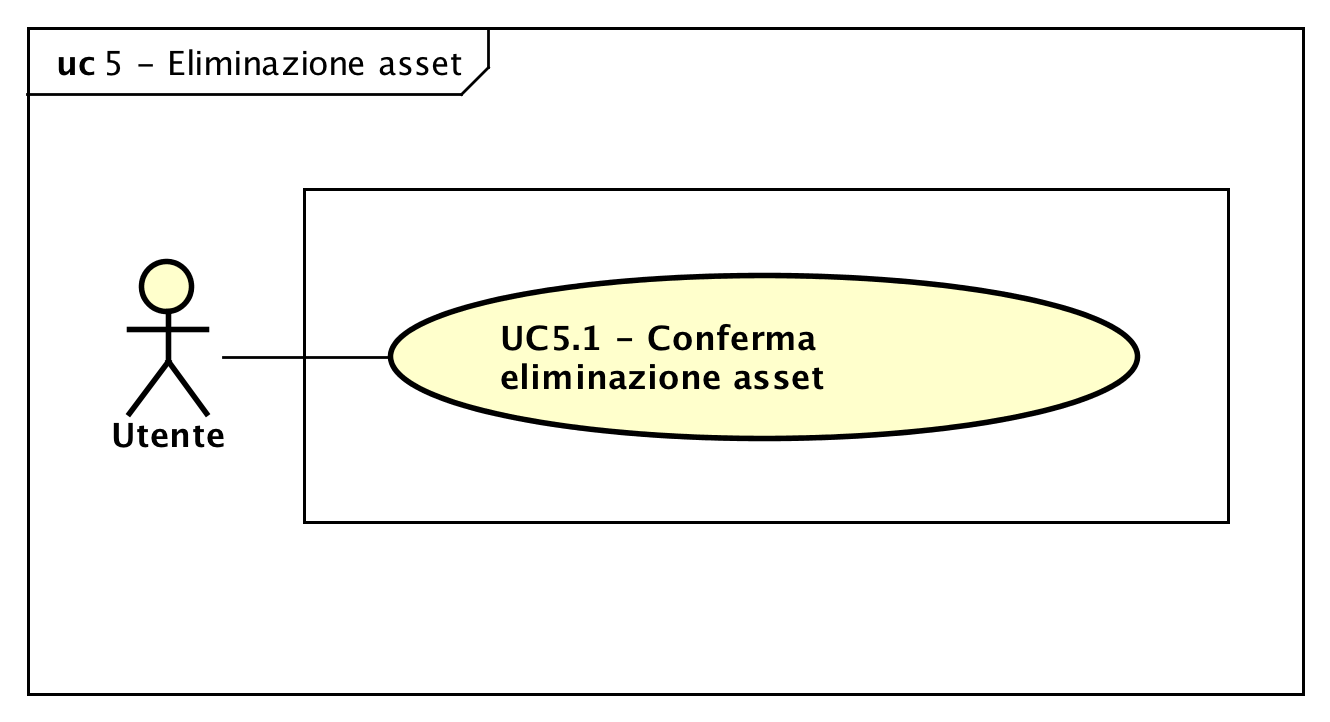
\includegraphics[scale=0.5]{{img/uc5}.png}
\caption{UC5 - Eliminazione asset}
\end{figure}
\def\arraystretch{1.5}
\rowcolors{2}{D}{P}
\begin{tabularx}{\textwidth}{l|p{0.7\textwidth}}
\rowcolor{I} \multicolumn{2}{c}{\color{white}\textbf{UC5 - Eliminazione asset}} \\
\toprule
\endhead
\textbf{Attori} & Utente\\
\textbf{Descrizione} & l'utente elimina un asset\\
\textbf{Pre-condizione} & l'utente ha aperto l'applicazione; è stato inserito almeno un asset; l'utente ha selezionato un asset\\
\textbf{Post-condizione} & l'asset è stato eliminato\\
\textbf{Scenario principale} & \vspace{-1.2em}\begin{enumerate}[leftmargin=*,noitemsep,nosep]
\item \nameref{sssec:UC5.1}.
\end{enumerate}\\
\textbf{Scenari alternativi} & \vspace{-1.2em}\begin{itemize}[leftmargin=*,noitemsep,nosep]
\item \nameref{sssec:UC5.2}.
\end{itemize}\\
%\textbf{Generalizzazioni} &  \\
\bottomrule
\end{tabularx}
\subsection{UC5.1 - Conferma eliminazione asset}
\label{sssec:UC5.1}
\def\arraystretch{1.5}
\rowcolors{2}{D}{P}
\begin{tabularx}{\textwidth}{l|p{0.7\textwidth}}
\rowcolor{I} \multicolumn{2}{c}{\color{white}\textbf{UC5.1 - Conferma eliminazione asset}} \\
\toprule
\endhead
\textbf{Attori} & Utente\\
\textbf{Descrizione} & l'utente conferma l'eliminazione dell'asset\\
\textbf{Pre-condizione} & il sistema offre la possibilità di confermare l'eliminazione dell'asset\\
\textbf{Post-condizione} & l'asset è stato eliminato\\
\textbf{Estensioni} & \vspace{-1.2em}\begin{itemize}[leftmargin=*,noitemsep,nosep]
\item \nameref{sssec:UC5.2}.
\end{itemize}\\
%\textbf{Generalizzazioni} &  \\
\bottomrule
\end{tabularx}
\subsection{UC5.2 - Interruzione eliminazione asset}
\label{sssec:UC5.2}
\def\arraystretch{1.5}
\rowcolors{2}{D}{P}
\begin{tabularx}{\textwidth}{l|p{0.7\textwidth}}
\rowcolor{I} \multicolumn{2}{c}{\color{white}\textbf{UC5.2 - Interruzione eliminazione asset}} \\
\toprule
\endhead
\textbf{Attori} & Utente\\
\textbf{Descrizione} & l'utente interrompe l'eliminazione dell'asset\\
\textbf{Pre-condizione} & il sistema offre la possibilità di confermare l'eliminazione dell'asset\\
\textbf{Post-condizione} & l'asset non è stato eliminato\\
%\textbf{Generalizzazioni} &  \\
\bottomrule
\end{tabularx}
\subsection{UC6 - Aggiunta nodo}
\label{sssec:UC6}
\begin{figure}[H]
\centering
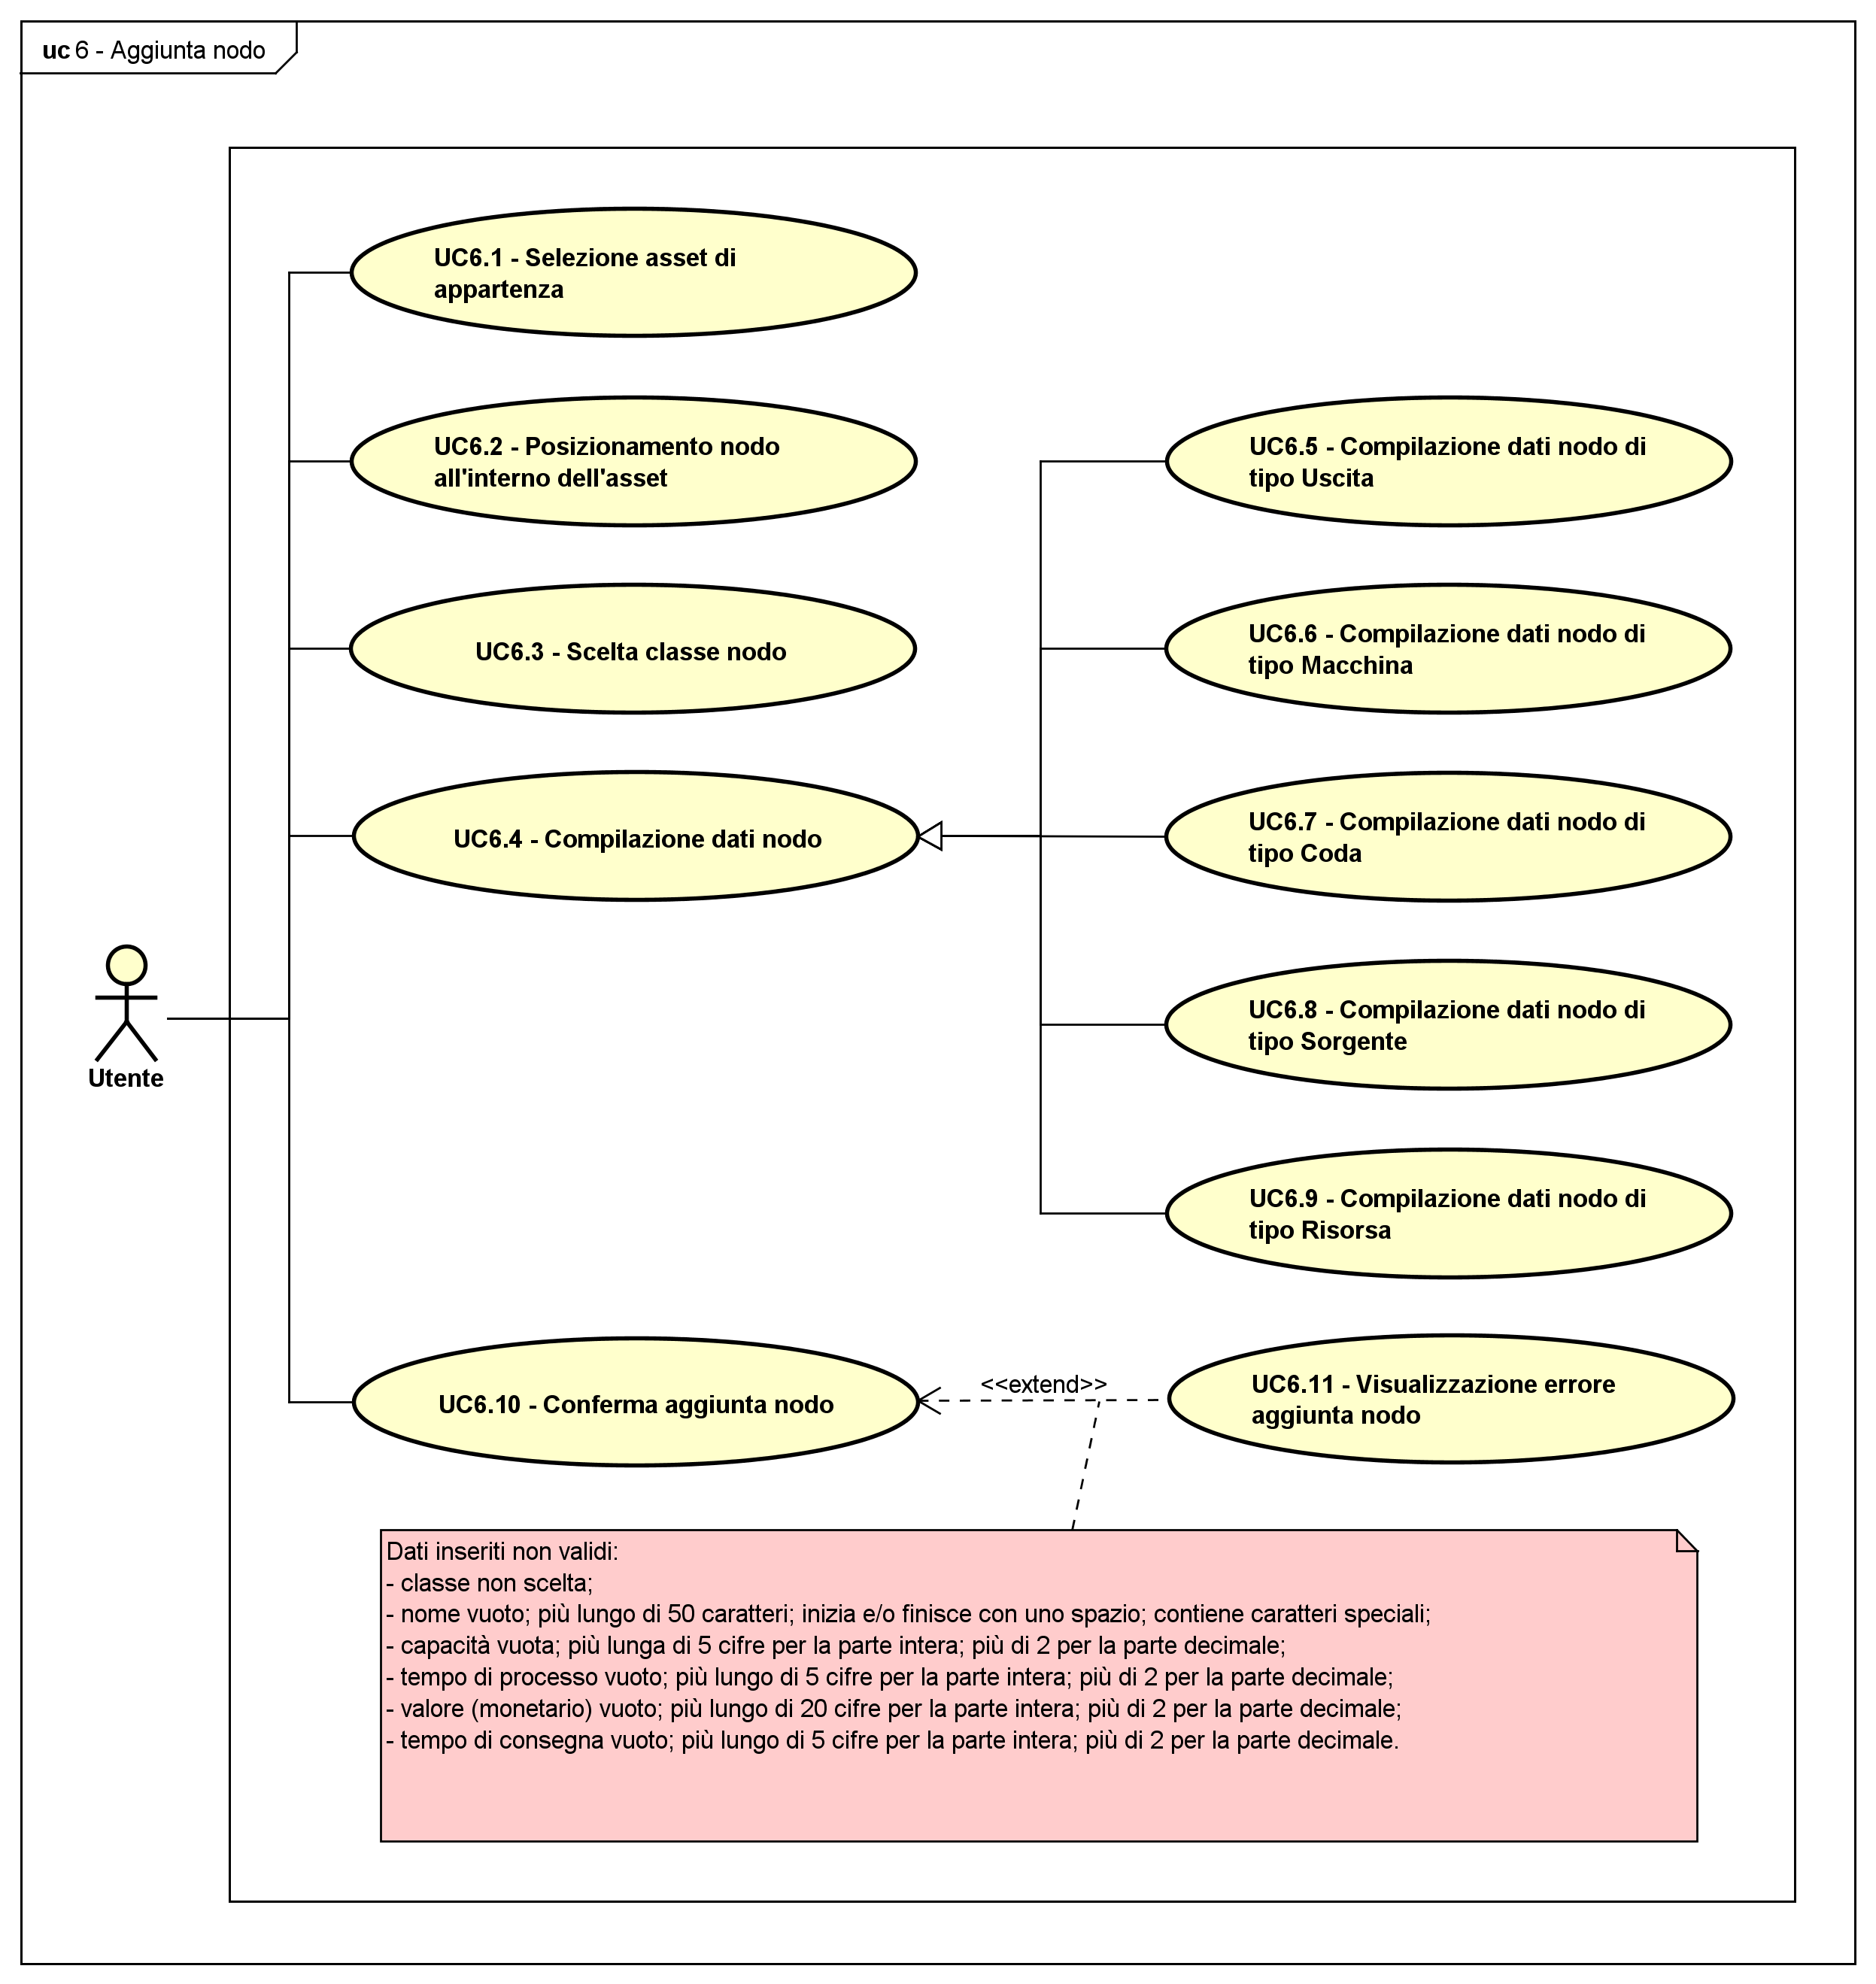
\includegraphics[width=\textwidth]{{img/uc6}.png}
\caption{UC6 - Aggiunta nodo}
\end{figure}
\def\arraystretch{1.5}
\rowcolors{2}{D}{P}
\begin{tabularx}{\textwidth}{l|p{0.7\textwidth}}
\rowcolor{I} \multicolumn{2}{c}{\color{white}\textbf{UC6 - Aggiunta nodo}} \\
\toprule
\endhead
\textbf{Attori} & Utente\\
\textbf{Descrizione} & l'utente aggiunge un nodo\\
\textbf{Pre-condizione} & l'utente ha aperto l'applicazione; è stato inserito almeno un asset\\
\textbf{Post-condizione} & un nuovo nodo è stato aggiunto\\
\textbf{Scenario principale} & \vspace{-1.2em}\begin{enumerate}[leftmargin=*,noitemsep,nosep]
\item \nameref{sssec:UC6.1};
\item \nameref{sssec:UC6.2};
\item \nameref{sssec:UC6.3};
\item \nameref{sssec:UC6.4};
\item \nameref{sssec:UC6.6}.
\end{enumerate}\\
\textbf{Scenari alternativi} & \vspace{-1.2em}\begin{itemize}[leftmargin=*,noitemsep,nosep]
\item \nameref{sssec:UC6.5};
\item \nameref{sssec:UC6.7}.
\end{itemize}\\
%\textbf{Generalizzazioni} &  \\
\bottomrule
\end{tabularx}
\subsection{UC6.1 - Selezione asset di appartenenza}
\label{sssec:UC6.1}
\def\arraystretch{1.5}
\rowcolors{2}{D}{P}
\begin{tabularx}{\textwidth}{l|p{0.7\textwidth}}
\rowcolor{I} \multicolumn{2}{c}{\color{white}\textbf{UC6.1 - Selezione asset di appartenenza}} \\
\toprule
\endhead
\textbf{Attori} & Utente\\
\textbf{Descrizione} & l'utente seleziona un asset\\
\textbf{Pre-condizione} & il sistema offre la possibilità di selezionare l'asset di appartenenza\\
\textbf{Post-condizione} & l'asset di appartenenza è stato selezionato\\
\textbf{Estensioni} & \vspace{-1.2em}\begin{itemize}[leftmargin=*,noitemsep,nosep]
\item \nameref{sssec:UC6.5}.
\end{itemize}\\
%\textbf{Generalizzazioni} &  \\
\bottomrule
\end{tabularx}
\subsection{UC6.2 - Posizionamento nodo all'interno dell'asset}
\label{sssec:UC6.2}
\def\arraystretch{1.5}
\rowcolors{2}{D}{P}
\begin{tabularx}{\textwidth}{l|p{0.7\textwidth}}
\rowcolor{I} \multicolumn{2}{c}{\color{white}\textbf{UC6.2 - Posizionamento nodo all'interno dell'asset}} \\
\toprule
\endhead
\textbf{Attori} & Utente\\
\textbf{Descrizione} & l'utente posiziona il nodo nella collocazione desiderata all'interno dell'asset\\
\textbf{Pre-condizione} & l'utente ha selezionato l'asset di appartenenza\\
\textbf{Post-condizione} & il nodo è stato posizionato all'interno dell'asset\\
\textbf{Estensioni} & \vspace{-1.2em}\begin{itemize}[leftmargin=*,noitemsep,nosep]
\item \nameref{sssec:UC6.5}.
\end{itemize}\\
%\textbf{Generalizzazioni} &  \\
\bottomrule
\end{tabularx}
\subsection{UC6.3 - Scelta classe nodo}
\label{sssec:UC6.3}
\def\arraystretch{1.5}
\rowcolors{2}{D}{P}
\begin{tabularx}{\textwidth}{l|p{0.7\textwidth}}
\rowcolor{I} \multicolumn{2}{c}{\color{white}\textbf{UC6.3 - Scelta classe nodo}} \\
\toprule
\endhead
\textbf{Attori} & Utente\\
\textbf{Descrizione} & l'utente sceglie la classe del nodo\\
\textbf{Pre-condizione} & l'utente ha posizionato il nodo all'interno dell'asset\\
\textbf{Post-condizione} & la classe del nodo è stata scelta\\
\textbf{Estensioni} & \vspace{-1.2em}\begin{itemize}[leftmargin=*,noitemsep,nosep]
\item \nameref{sssec:UC6.5}.
\end{itemize}\\
%\textbf{Generalizzazioni} &  \\
\bottomrule
\end{tabularx}
\subsection{UC6.4 - Compilazione dati nodo}
\label{sssec:UC6.4}
\begin{figure}[H]
\centering
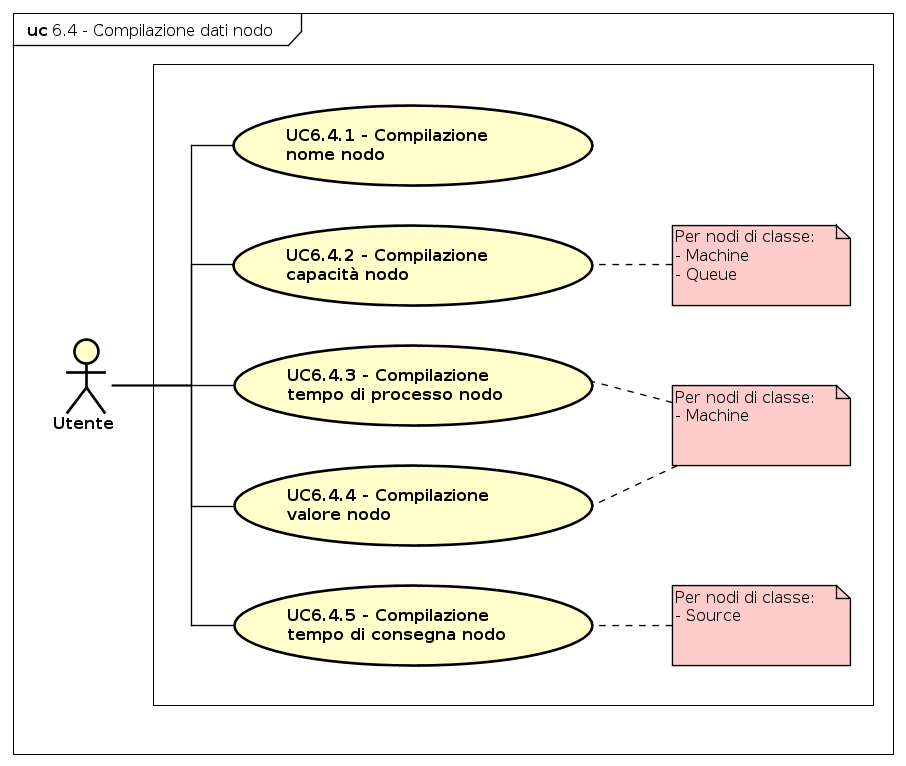
\includegraphics[scale=0.5]{{img/uc6.4}.png}
\caption{UC6.4 - Compilazione dati nodo}
\end{figure}
\def\arraystretch{1.5}
\rowcolors{2}{D}{P}
\begin{tabularx}{\textwidth}{l|p{0.7\textwidth}}
\rowcolor{I} \multicolumn{2}{c}{\color{white}\textbf{UC6.4 - Compilazione dati nodo}} \\
\toprule
\endhead
\textbf{Attori} & Utente\\
\textbf{Descrizione} & l'utente compila i dati del nodo\\
\textbf{Pre-condizione} & l'utente ha posizionato il nodo\\
\textbf{Post-condizione} & i dati del nodo sono stati compilati\\
\textbf{Scenario principale} & \vspace{-1.2em}\begin{enumerate}[leftmargin=*,noitemsep,nosep]
\item \nameref{sssec:UC6.4.1};
\item \nameref{sssec:UC6.4.2};
\item \nameref{sssec:UC6.4.3};
\item \nameref{sssec:UC6.4.4};
\item \nameref{sssec:UC6.4.5}.
\end{enumerate}\\
\textbf{Estensioni} & \vspace{-1.2em}\begin{itemize}[leftmargin=*,noitemsep,nosep]
\item \nameref{sssec:UC6.5}.
\end{itemize}\\
%\textbf{Generalizzazioni} &  \\
\bottomrule
\end{tabularx}
\subsection{UC6.4.1 - Compilazione nome nodo}
\label{sssec:UC6.4.1}
\def\arraystretch{1.5}
\rowcolors{2}{D}{P}
\begin{tabularx}{\textwidth}{l|p{0.7\textwidth}}
\rowcolor{I} \multicolumn{2}{c}{\color{white}\textbf{UC6.4.1 - Compilazione nome nodo}} \\
\toprule
\endhead
\textbf{Attori} & Utente\\
\textbf{Descrizione} & l'utente compila il nome del nodo\\
\textbf{Pre-condizione} & il sistema offre la possibilità di compilare il nome del nodo\\
\textbf{Post-condizione} & l'utente ha compilato il nome del nodo\\
%\textbf{Generalizzazioni} &  \\
\bottomrule
\end{tabularx}
\subsection{UC6.4.2 - Compilazione capacità nodo}
\label{sssec:UC6.4.2}
\def\arraystretch{1.5}
\rowcolors{2}{D}{P}
\begin{tabularx}{\textwidth}{l|p{0.7\textwidth}}
\rowcolor{I} \multicolumn{2}{c}{\color{white}\textbf{UC6.4.2 - Compilazione capacità nodo}} \\
\toprule
\endhead
\textbf{Attori} & Utente\\
\textbf{Descrizione} & l'utente compila la capacità del nodo\\
\textbf{Pre-condizione} & l'utente ha scelto come classe del nodo Macchina o Coda\\
\textbf{Post-condizione} & la capacità del nodo è stata compilata\\
%\textbf{Generalizzazioni} &  \\
\bottomrule
\end{tabularx}
\subsection{UC6.4.3 - Compilazione tempo di processo nodo}
\label{sssec:UC6.4.3}
\def\arraystretch{1.5}
\rowcolors{2}{D}{P}
\begin{tabularx}{\textwidth}{l|p{0.7\textwidth}}
\rowcolor{I} \multicolumn{2}{c}{\color{white}\textbf{UC6.4.3 - Compilazione tempo di processo nodo}} \\
\toprule
\endhead
\textbf{Attori} & Utente\\
\textbf{Descrizione} & l'utente compila il tempo di processo del nodo\\
\textbf{Pre-condizione} & l'utente ha scelto come classe del nodo Macchina\\
\textbf{Post-condizione} & il tempo di processo del nodo è stato compilato\\
%\textbf{Generalizzazioni} &  \\
\bottomrule
\end{tabularx}
\subsection{UC6.4.4 - Compilazione valore nodo}
\label{sssec:UC6.4.4}
\def\arraystretch{1.5}
\rowcolors{2}{D}{P}
\begin{tabularx}{\textwidth}{l|p{0.7\textwidth}}
\rowcolor{I} \multicolumn{2}{c}{\color{white}\textbf{UC6.4.4 - Compilazione valore nodo}} \\
\toprule
\endhead
\textbf{Attori} & Utente\\
\textbf{Descrizione} & l'utente compila il valore del nodo\\
\textbf{Pre-condizione} & l'utente ha scelto come classe del nodo Macchina\\
\textbf{Post-condizione} & il valore del nodo è stato compilato\\
%\textbf{Generalizzazioni} &  \\
\bottomrule
\end{tabularx}
\subsection{UC6.4.5 - Compilazione tempo di consegna nodo}
\label{sssec:UC6.4.5}
\def\arraystretch{1.5}
\rowcolors{2}{D}{P}
\begin{tabularx}{\textwidth}{l|p{0.7\textwidth}}
\rowcolor{I} \multicolumn{2}{c}{\color{white}\textbf{UC6.4.5 - Compilazione tempo di consegna nodo}} \\
\toprule
\endhead
\textbf{Attori} & Utente\\
\textbf{Descrizione} & l'utente compila il tempo di consegna del nodo\\
\textbf{Pre-condizione} & l'utente ha scelto come classe del nodo Sorgente\\
\textbf{Post-condizione} & il tempo di consegna del nodo è stato compilato\\
%\textbf{Generalizzazioni} &  \\
\bottomrule
\end{tabularx}
\subsection{UC6.5 - Interruzione aggiunta nodo}
\label{sssec:UC6.5}
\def\arraystretch{1.5}
\rowcolors{2}{D}{P}
\begin{tabularx}{\textwidth}{l|p{0.7\textwidth}}
\rowcolor{I} \multicolumn{2}{c}{\color{white}\textbf{UC6.5 - Interruzione aggiunta nodo}} \\
\toprule
\endhead
\textbf{Attori} & Utente\\
\textbf{Descrizione} & l'utente interrompe l'aggiunta di un nodo\\
\textbf{Pre-condizione} & il sistema offre la possibilità di aggiungere un nodo\\
\textbf{Post-condizione} & nessun nuovo nodo è stato aggiunto\\
%\textbf{Generalizzazioni} &  \\
\bottomrule
\end{tabularx}
\subsection{UC6.6 - Conferma aggiunta nodo}
\label{sssec:UC6.6}
\def\arraystretch{1.5}
\rowcolors{2}{D}{P}
\begin{tabularx}{\textwidth}{l|p{0.7\textwidth}}
\rowcolor{I} \multicolumn{2}{c}{\color{white}\textbf{UC6.6 - Conferma aggiunta nodo}} \\
\toprule
\endhead
\textbf{Attori} & Utente\\
\textbf{Descrizione} & l'utente conferma l'aggiunta di un nodo\\
\textbf{Pre-condizione} & il sistema offre la possibilità di confermare l'aggiunta di un nodo\\
\textbf{Post-condizione} & un nuovo nodo è stato aggiunto\\
\textbf{Estensioni} & \vspace{-1.2em}\begin{itemize}[leftmargin=*,noitemsep,nosep]
\item \nameref{sssec:UC6.7}.
\end{itemize}\\
%\textbf{Generalizzazioni} &  \\
\bottomrule
\end{tabularx}
\subsection{UC6.7 - Visualizzazione errore aggiunta nodo}
\label{sssec:UC6.7}
\def\arraystretch{1.5}
\rowcolors{2}{D}{P}
\begin{tabularx}{\textwidth}{l|p{0.7\textwidth}}
\rowcolor{I} \multicolumn{2}{c}{\color{white}\textbf{UC6.7 - Visualizzazione errore aggiunta nodo}} \\
\toprule
\endhead
\textbf{Attori} & Utente\\
\textbf{Descrizione} & l'utente visualizza un errore relativo ai dati del nodo compilati in modo errato\\
\textbf{Pre-condizione} & l'utente sta tentando di inserire un nuovo nodo\\
\textbf{Post-condizione} & nessun nuovo nodo aggiunto; l'utente visualizza un errore relativo ai dati del nodo compilati in modo errato\\
%\textbf{Generalizzazioni} &  \\
\bottomrule
\end{tabularx}
\subsection{UC7 - Visualizzazione info nodo}
\label{sssec:UC7}
\def\arraystretch{1.5}
\rowcolors{2}{D}{P}
\begin{tabularx}{\textwidth}{l|p{0.7\textwidth}}
\rowcolor{I} \multicolumn{2}{c}{\color{white}\textbf{UC7 - Visualizzazione info nodo}} \\
\toprule
\endhead
\textbf{Attori} & Utente\\
\textbf{Descrizione} & l'utente seleziona un nodo e ne visualizza le informazioni\\
\textbf{Pre-condizione} & l'utente ha aperto l'applicazione; è stato inserito almeno un nodo\\
\textbf{Post-condizione} & il sistema mostra le informazioni dell'asset selezionato\\
%\textbf{Generalizzazioni} &  \\
\bottomrule
\end{tabularx}
\subsection{UC8 - Chiusura visualizzazione info nodo}
\label{sssec:UC8}
\def\arraystretch{1.5}
\rowcolors{2}{D}{P}
\begin{tabularx}{\textwidth}{l|p{0.7\textwidth}}
\rowcolor{I} \multicolumn{2}{c}{\color{white}\textbf{UC8 - Chiusura visualizzazione info nodo}} \\
\toprule
\endhead
\textbf{Attori} & Utente\\
\textbf{Descrizione} & l'utente chiude la visualizzazione delle informazioni di un nodo\\
\textbf{Pre-condizione} & l'utente ha visualizzato le informazioni di un nodo\\
\textbf{Post-condizione} & è stata chiusa la visualizzazione delle informazioni di un nodo\\
%\textbf{Generalizzazioni} &  \\
\bottomrule
\end{tabularx}
\subsection{UC9 - Modifica nodo}
\label{sssec:UC9}
\begin{figure}[H]
\centering
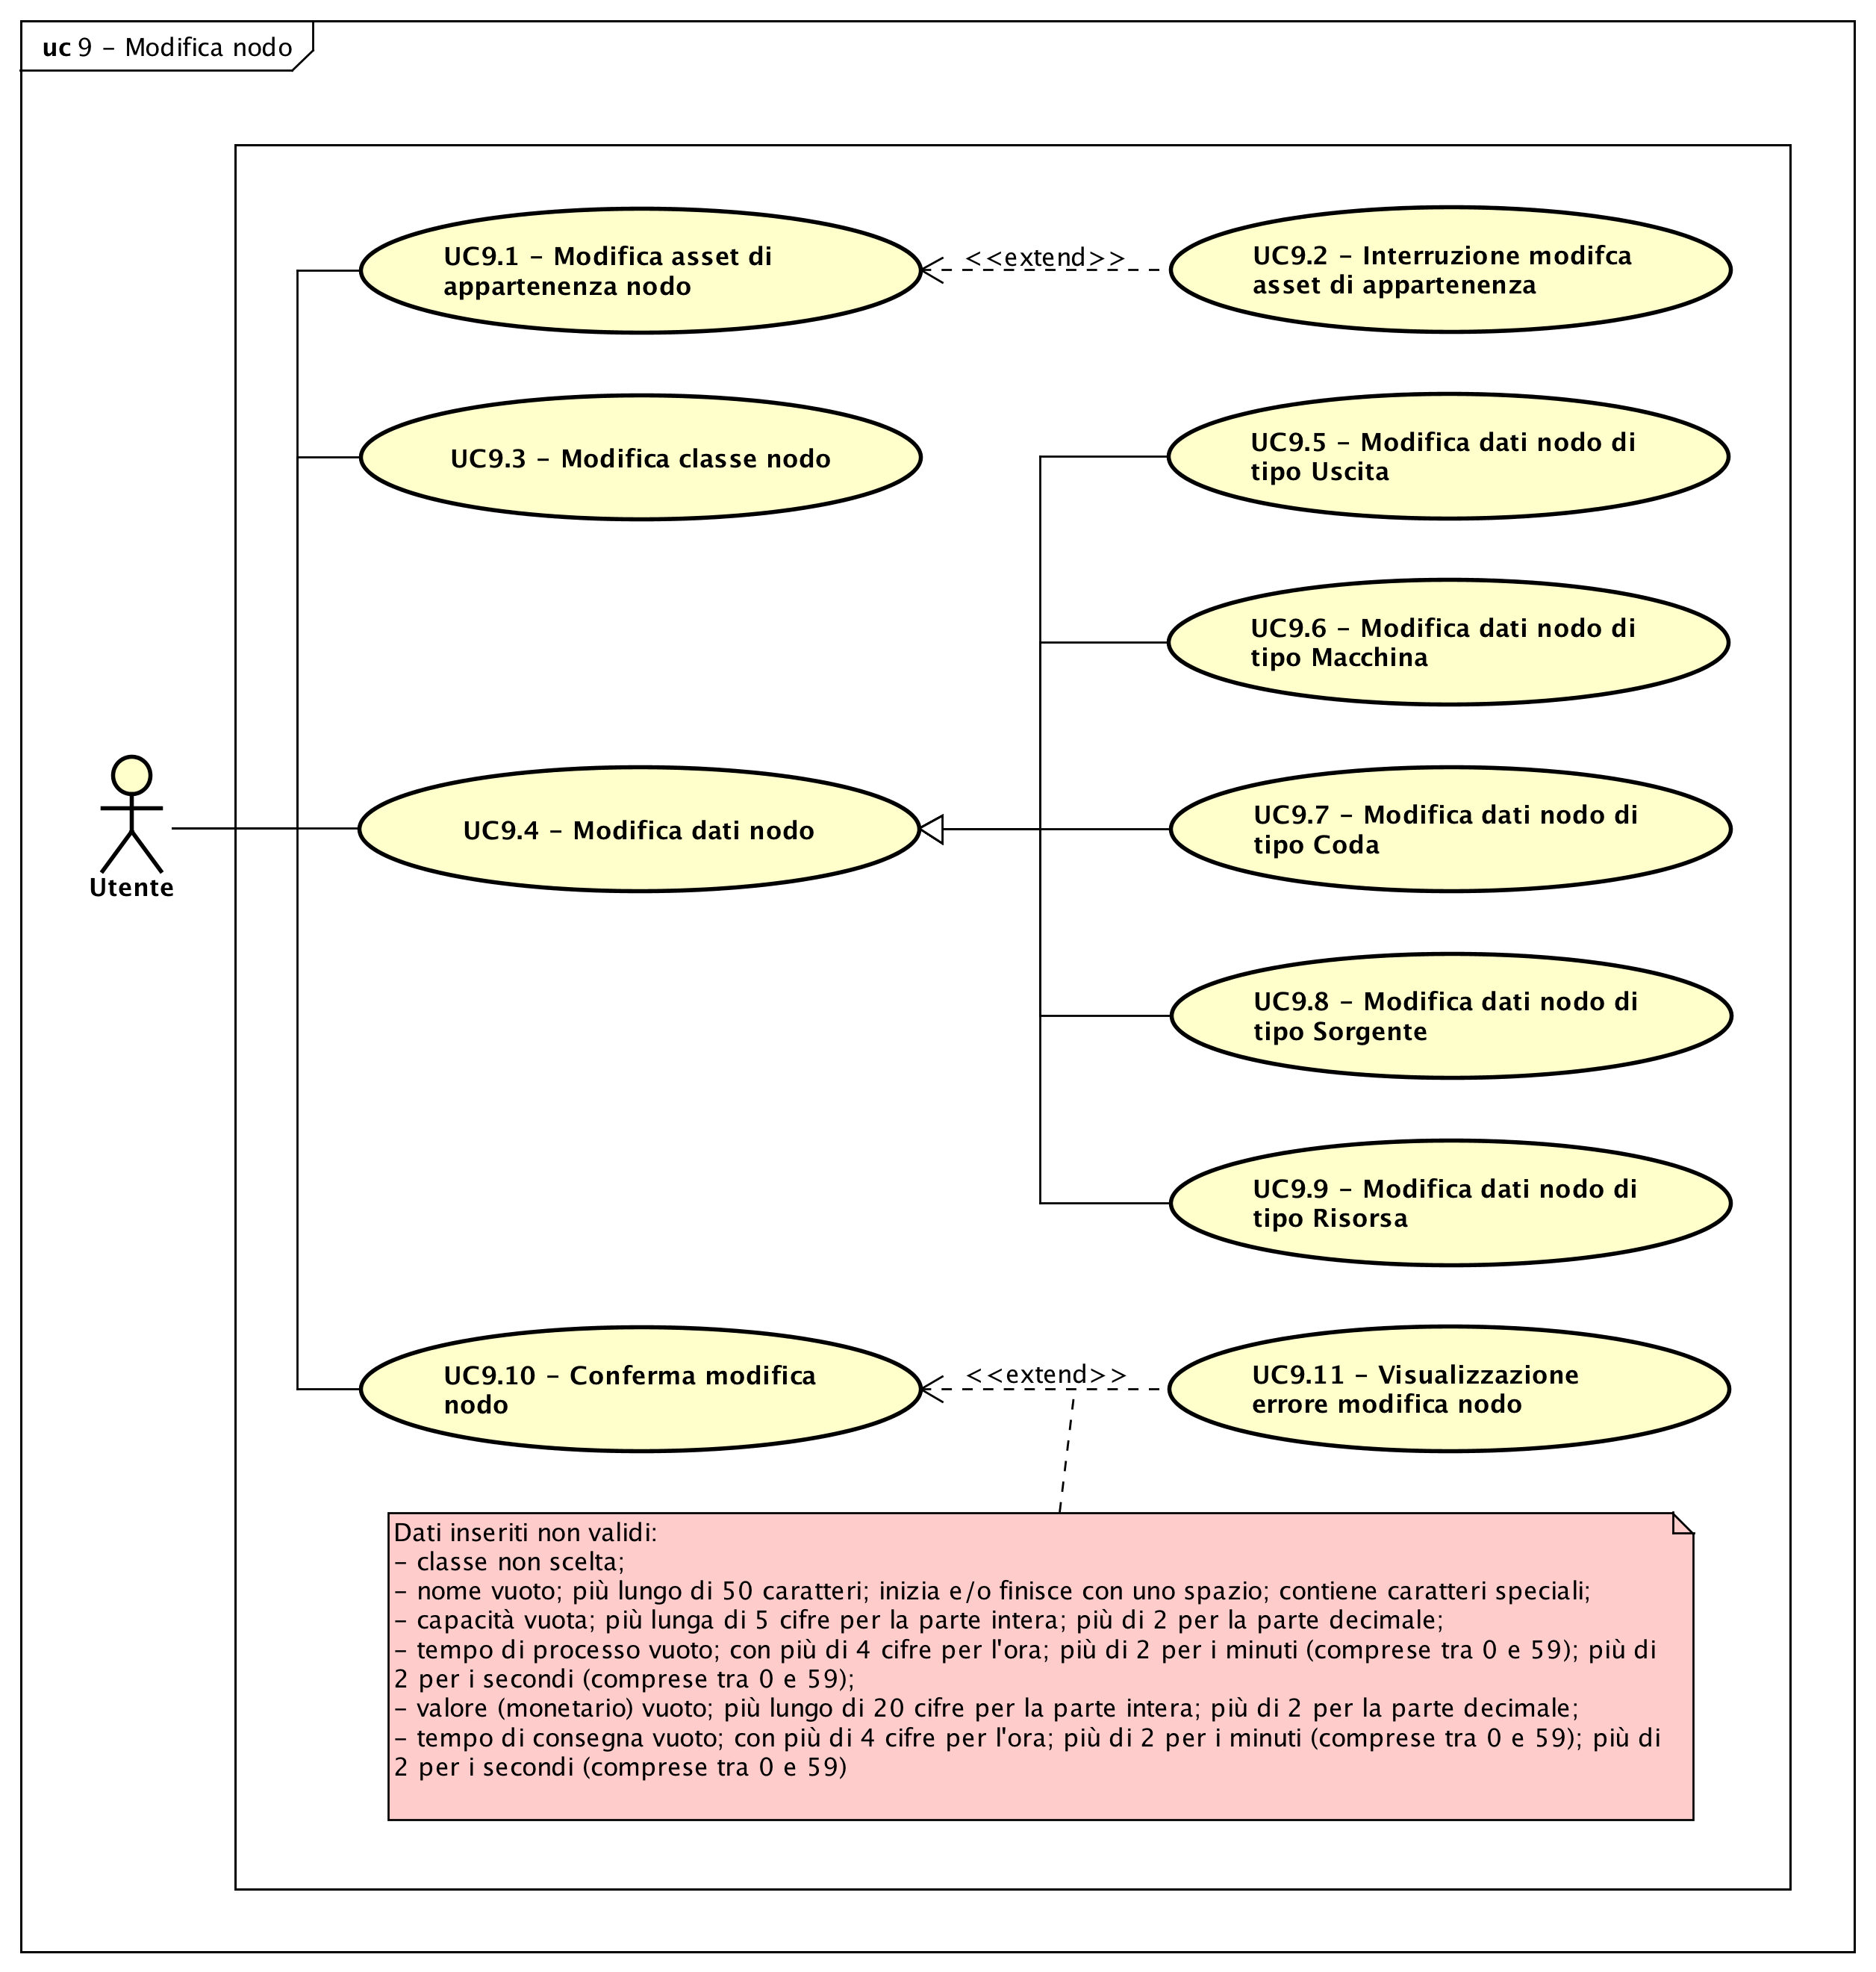
\includegraphics[width=\textwidth]{{img/uc9}.png}
\caption{UC9 - Modifica nodo}
\end{figure}
\def\arraystretch{1.5}
\rowcolors{2}{D}{P}
\begin{tabularx}{\textwidth}{l|p{0.7\textwidth}}
\rowcolor{I} \multicolumn{2}{c}{\color{white}\textbf{UC9 - Modifica nodo}} \\
\toprule
\endhead
\textbf{Attori} & Utente\\
\textbf{Descrizione} & l'utente modifica il nodo\\
\textbf{Pre-condizione} & l'utente ha aperto l'applicazione; almeno un nodo è stato aggiunto; l'utente ha selezionato un nodo\\
\textbf{Post-condizione} & il nodo è stato modificato\\
\textbf{Scenario principale} & \vspace{-1.2em}\begin{enumerate}[leftmargin=*,noitemsep,nosep]
\item \nameref{sssec:UC9.1};
\item \nameref{sssec:UC9.3};
\item \nameref{sssec:UC9.5};
\item \nameref{sssec:UC9.6}.
\end{enumerate}\\
\textbf{Scenari alternativi} & \vspace{-1.2em}\begin{itemize}[leftmargin=*,noitemsep,nosep]
\item \nameref{sssec:UC9.2};
\item \nameref{sssec:UC9.4};
\item \nameref{sssec:UC9.7}.
\end{itemize}\\
%\textbf{Generalizzazioni} &  \\
\bottomrule
\end{tabularx}
\subsection{UC9.1 - Modifica asset di appartenenza nodo}
\label{sssec:UC9.1}
\begin{figure}[H]
\centering
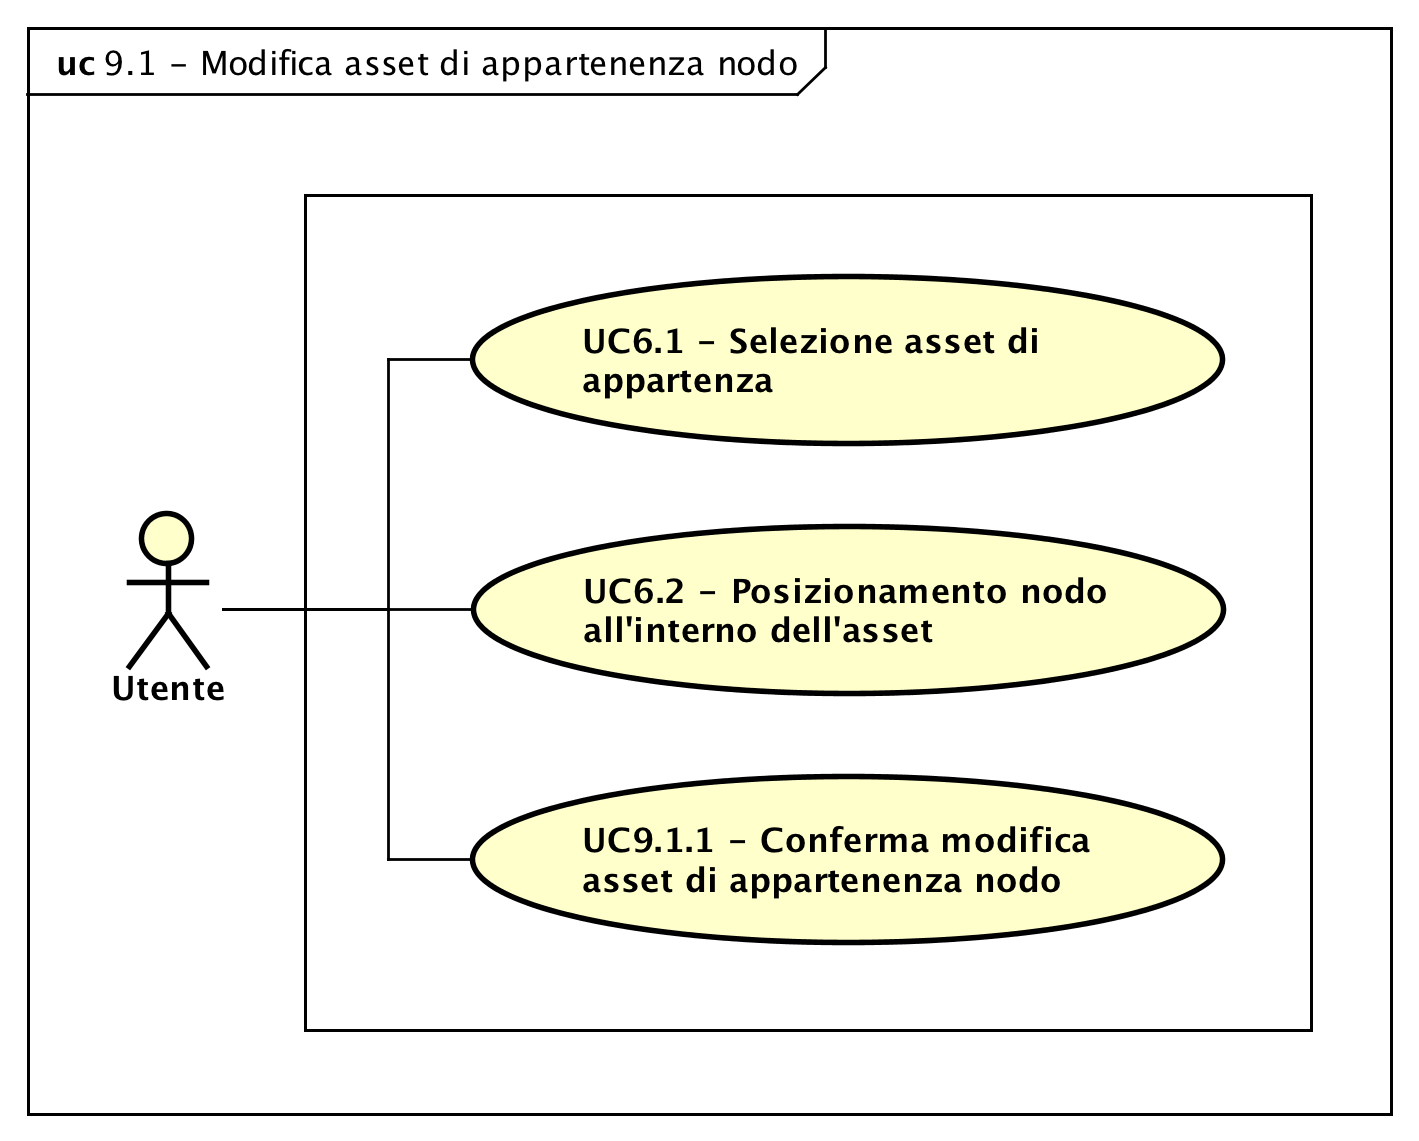
\includegraphics[scale=0.5]{{img/uc9.1}.png}
\caption{UC9.1 - Modifica asset di appartenenza nodo}
\end{figure}
\def\arraystretch{1.5}
\rowcolors{2}{D}{P}
\begin{tabularx}{\textwidth}{l|p{0.7\textwidth}}
\rowcolor{I} \multicolumn{2}{c}{\color{white}\textbf{UC9.1 - Modifica asset di appartenenza nodo}} \\
\toprule
\endhead
\textbf{Attori} & Utente\\
\textbf{Descrizione} & l'utente modifica l'asset di appartenenza del nodo\\
\textbf{Pre-condizione} & il sistema offre la possibilità di modificare l'asset di appartenenza del nodo\\
\textbf{Post-condizione} & l'asset di appartenenza del nodo è stato modificato\\
\textbf{Scenario principale} & \vspace{-1.2em}\begin{enumerate}[leftmargin=*,noitemsep,nosep]
\item \nameref{sssec:UC6.1};
\item \nameref{sssec:UC6.2};
\end{enumerate}\\
\textbf{Estensioni} & \vspace{-1.2em}\begin{itemize}[leftmargin=*,noitemsep,nosep]
\item \nameref{sssec:UC9.2}.
\end{itemize}\\
%\textbf{Generalizzazioni} &  \\
\bottomrule
\end{tabularx}
\subsection{UC9.1.1 - Conferma modifica asset di appartenenza nodo}
\label{sssec:UC9.1.1}
\def\arraystretch{1.5}
\rowcolors{2}{D}{P}
\begin{tabularx}{\textwidth}{l|p{0.7\textwidth}}
\rowcolor{I} \multicolumn{2}{c}{\color{white}\textbf{UC9.1.1 - Conferma modifica asset di appartenenza nodo}} \\
\toprule
\endhead
\textbf{Attori} & Utente\\
\textbf{Descrizione} & l'utente conferma la modifica dell'asset di appartenenza del nodo\\
\textbf{Pre-condizione} & il sistema offre la possibilità di confermare l'asset di appartenenza del nodo\\
\textbf{Post-condizione} & l'asset di appartenenza del nodo è stato modificato\\
%\textbf{Generalizzazioni} &  \\
\bottomrule
\end{tabularx}
\subsection{UC9.2 - Interruzione modifica asset di appartenenza}
\label{sssec:UC9.2}
\def\arraystretch{1.5}
\rowcolors{2}{D}{P}
\begin{tabularx}{\textwidth}{l|p{0.7\textwidth}}
\rowcolor{I} \multicolumn{2}{c}{\color{white}\textbf{UC9.2 - Interruzione modifica asset di appartenenza}} \\
\toprule
\endhead
\textbf{Attori} & Utente\\
\textbf{Descrizione} & l'utente interrompe la modifica dell'asset di appartenenza del nodo\\
\textbf{Pre-condizione} & il sistema offre la possibilità di modificare l'asset di appartenenza\\
\textbf{Post-condizione} & l'asset di appartenenza del nodo non è stato modificato; l'utente può modificare altri dati\\
%\textbf{Generalizzazioni} &  \\
\bottomrule
\end{tabularx}
\subsection{UC9.3 - Modifica classe nodo}
\label{sssec:UC9.3}
\def\arraystretch{1.5}
\rowcolors{2}{D}{P}
\begin{tabularx}{\textwidth}{l|p{0.7\textwidth}}
\rowcolor{I} \multicolumn{2}{c}{\color{white}\textbf{UC9.3 - Modifica classe nodo}} \\
\toprule
\endhead
\textbf{Attori} & Utente\\
\textbf{Descrizione} & l'utente modifica la classe del nodo\\
\textbf{Pre-condizione} & il sistema offre la possibilità di modificare la classe del nodo\\
\textbf{Post-condizione} & la classe del nodo è stata modificata\\
\textbf{Estensioni} & \vspace{-1.2em}\begin{itemize}[leftmargin=*,noitemsep,nosep]
\item \nameref{sssec:UC9.4}.
\end{itemize}\\
%\textbf{Generalizzazioni} &  \\
\bottomrule
\end{tabularx}
\subsection{UC9.4 - Interruzione modifica nodo}
\label{sssec:UC9.4}
\def\arraystretch{1.5}
\rowcolors{2}{D}{P}
\begin{tabularx}{\textwidth}{l|p{0.7\textwidth}}
\rowcolor{I} \multicolumn{2}{c}{\color{white}\textbf{UC9.4 - Interruzione modifica nodo}} \\
\toprule
\endhead
\textbf{Attori} & Utente\\
\textbf{Descrizione} & l'utente interrompe la modifica del nodo\\
\textbf{Pre-condizione} & il sistema offre la possibilità di modificare un nodo\\
\textbf{Post-condizione} & il nodo non è stato modificato\\
%\textbf{Generalizzazioni} &  \\
\bottomrule
\end{tabularx}
\subsection{UC9.5 - Modifica dati nodo}
\label{sssec:UC9.5}
\begin{figure}[H]
\centering
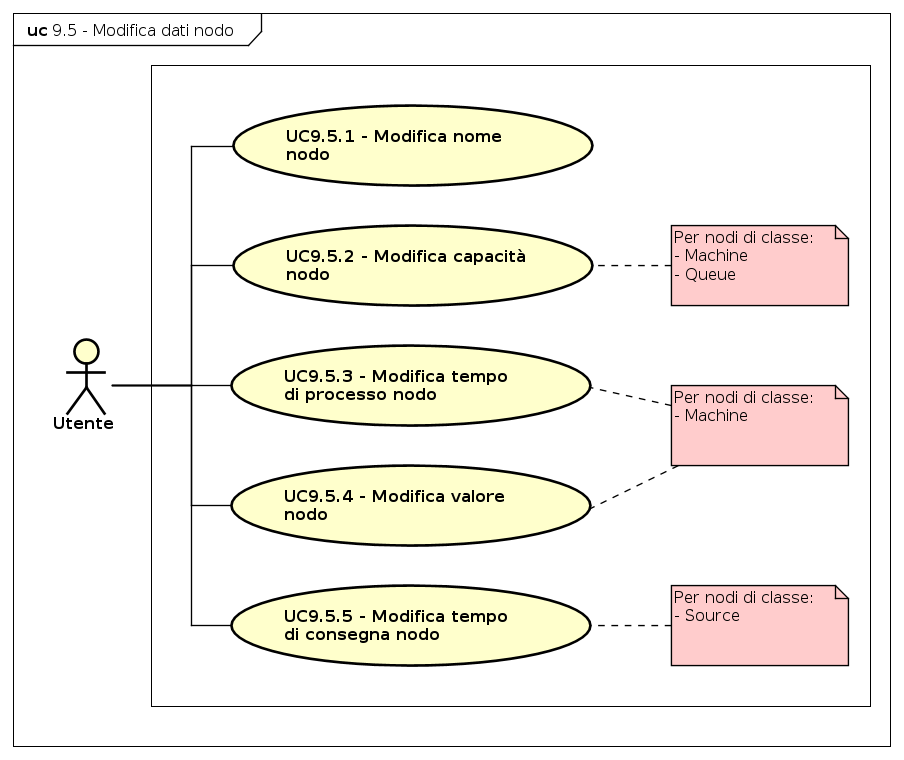
\includegraphics[scale=0.5]{{img/uc9.5}.png}
\caption{UC9.5 - Modifica dati nodo}
\end{figure}
\def\arraystretch{1.5}
\rowcolors{2}{D}{P}
\begin{tabularx}{\textwidth}{l|p{0.7\textwidth}}
\rowcolor{I} \multicolumn{2}{c}{\color{white}\textbf{UC9.5 - Modifica dati nodo}} \\
\toprule
\endhead
\textbf{Attori} & Utente\\
\textbf{Descrizione} & l'utente modifica i dati del nodo\\
\textbf{Pre-condizione} & il sistema offre la possibilità di modificare i dati del nodo\\
\textbf{Post-condizione} & i dati del nodo sono stati modificati\\
\textbf{Scenario principale} & \vspace{-1.2em}\begin{enumerate}[leftmargin=*,noitemsep,nosep]
\item \nameref{sssec:UC9.5.1};
\item \nameref{sssec:UC9.5.2};
\item \nameref{sssec:UC9.5.3};
\item \nameref{sssec:UC9.5.4};
\item \nameref{sssec:UC9.5.5}.
\end{enumerate}\\
\textbf{Estensioni} & \vspace{-1.2em}\begin{itemize}[leftmargin=*,noitemsep,nosep]
\item \nameref{sssec:UC9.4}.
\end{itemize}\\
%\textbf{Generalizzazioni} &  \\
\bottomrule
\end{tabularx}
\subsection{UC9.5.1 - Modifica nome nodo}
\label{sssec:UC9.5.1}
\def\arraystretch{1.5}
\rowcolors{2}{D}{P}
\begin{tabularx}{\textwidth}{l|p{0.7\textwidth}}
\rowcolor{I} \multicolumn{2}{c}{\color{white}\textbf{UC9.5.1 - Modifica nome nodo}} \\
\toprule
\endhead
\textbf{Attori} & Utente\\
\textbf{Descrizione} & l'utente modifica il campo relativo al nome del nodo\\
\textbf{Pre-condizione} & il sistema offre la possibilità di modificare il nome del nodo\\
\textbf{Post-condizione} & il campo relativo al nome del nodo è stato modificato\\
%\textbf{Generalizzazioni} &  \\
\bottomrule
\end{tabularx}
\subsection{UC9.5.2 - Modifica capacità nodo}
\label{sssec:UC9.5.2}
\def\arraystretch{1.5}
\rowcolors{2}{D}{P}
\begin{tabularx}{\textwidth}{l|p{0.7\textwidth}}
\rowcolor{I} \multicolumn{2}{c}{\color{white}\textbf{UC9.5.2 - Modifica capacità nodo}} \\
\toprule
\endhead
\textbf{Attori} & Utente\\
\textbf{Descrizione} & l'utente modifica il campo relativo alla capacità del nodo\\
\textbf{Pre-condizione} & il sistema offre la possibilità di modificare la capacità del nodo; l'utente ha scelto come classe del nodo Macchina o Coda\\
\textbf{Post-condizione} & il campo relativo alla capacità del nodo è stato modificato\\
%\textbf{Generalizzazioni} &  \\
\bottomrule
\end{tabularx}
\subsection{UC9.5.3 - Modifica tempo di processo nodo}
\label{sssec:UC9.5.3}
\def\arraystretch{1.5}
\rowcolors{2}{D}{P}
\begin{tabularx}{\textwidth}{l|p{0.7\textwidth}}
\rowcolor{I} \multicolumn{2}{c}{\color{white}\textbf{UC9.5.3 - Modifica tempo di processo nodo}} \\
\toprule
\endhead
\textbf{Attori} & Utente\\
\textbf{Descrizione} & l'utente modifica il campo relativo al tempo di processo del nodo\\
\textbf{Pre-condizione} & il sistema offre la possibilità di modificare il tempo di processo del nodo; l'utente ha scelto come classe del nodo Macchina\\
\textbf{Post-condizione} & il campo relativo al tempo di processo del nodo è stato modificato\\
%\textbf{Generalizzazioni} &  \\
\bottomrule
\end{tabularx}
\subsection{UC9.5.4 - Modifica valore nodo}
\label{sssec:UC9.5.4}
\def\arraystretch{1.5}
\rowcolors{2}{D}{P}
\begin{tabularx}{\textwidth}{l|p{0.7\textwidth}}
\rowcolor{I} \multicolumn{2}{c}{\color{white}\textbf{UC9.5.4 - Modifica valore nodo}} \\
\toprule
\endhead
\textbf{Attori} & Utente\\
\textbf{Descrizione} & l'utente modifica il campo relativo al valore del nodo\\
\textbf{Pre-condizione} & il sistema offre la possibilità di modificare il valore del nodo; l'utente ha scelto come classe del nodo Macchina\\
\textbf{Post-condizione} & il campo relativo al valore del nodo è stato modificato\\
%\textbf{Generalizzazioni} &  \\
\bottomrule
\end{tabularx}
\subsection{UC9.5.5 - Modifica tempo di consegna nodo}
\label{sssec:UC9.5.5}
\def\arraystretch{1.5}
\rowcolors{2}{D}{P}
\begin{tabularx}{\textwidth}{l|p{0.7\textwidth}}
\rowcolor{I} \multicolumn{2}{c}{\color{white}\textbf{UC9.5.5 - Modifica tempo di consegna nodo}} \\
\toprule
\endhead
\textbf{Attori} & Utente\\
\textbf{Descrizione} & l'utente modifica il campo relativo al  tempo di consegna del nodo\\
\textbf{Pre-condizione} & il sistema offre la possibilità di modificare il tempo di consegna del nodo; l'utente ha scelto come classe del nodo Sorgente\\
\textbf{Post-condizione} & il campo relativo al tempo di consegna del nodo è stato modificato\\
%\textbf{Generalizzazioni} &  \\
\bottomrule
\end{tabularx}
\subsection{UC9.6 - Conferma modifica nodo}
\label{sssec:UC9.6}
\def\arraystretch{1.5}
\rowcolors{2}{D}{P}
\begin{tabularx}{\textwidth}{l|p{0.7\textwidth}}
\rowcolor{I} \multicolumn{2}{c}{\color{white}\textbf{UC9.6 - Conferma modifica nodo}} \\
\toprule
\endhead
\textbf{Attori} & Utente\\
\textbf{Descrizione} & l'utente conferma la modifica del nodo\\
\textbf{Pre-condizione} & il sistema offre la possibilità di confermare la modifica del nodo\\
\textbf{Post-condizione} & il nodo è stato modificato\\
\textbf{Estensioni} & \vspace{-1.2em}\begin{itemize}[leftmargin=*,noitemsep,nosep]
\item \nameref{sssec:UC9.7}.
\end{itemize}\\
%\textbf{Generalizzazioni} &  \\
\bottomrule
\end{tabularx}
\subsection{UC9.7 - Visualizzazione errore modifica nodo}
\label{sssec:UC9.7}
\def\arraystretch{1.5}
\rowcolors{2}{D}{P}
\begin{tabularx}{\textwidth}{l|p{0.7\textwidth}}
\rowcolor{I} \multicolumn{2}{c}{\color{white}\textbf{UC9.7 - Visualizzazione errore modifica nodo}} \\
\toprule
\endhead
\textbf{Attori} & Utente\\
\textbf{Descrizione} & l'utente visualizza un errore relativo alla modifica del nodo\\
\textbf{Pre-condizione} & l'utente ha confermato la modifica dei dati del nodo\\
\textbf{Post-condizione} & il nodo non è stato modificato e l'utente visualizza un errore\\
%\textbf{Generalizzazioni} &  \\
\bottomrule
\end{tabularx}
\subsection{UC10 - Eliminazione nodo}
\label{sssec:UC10}
\begin{figure}[H]
\centering
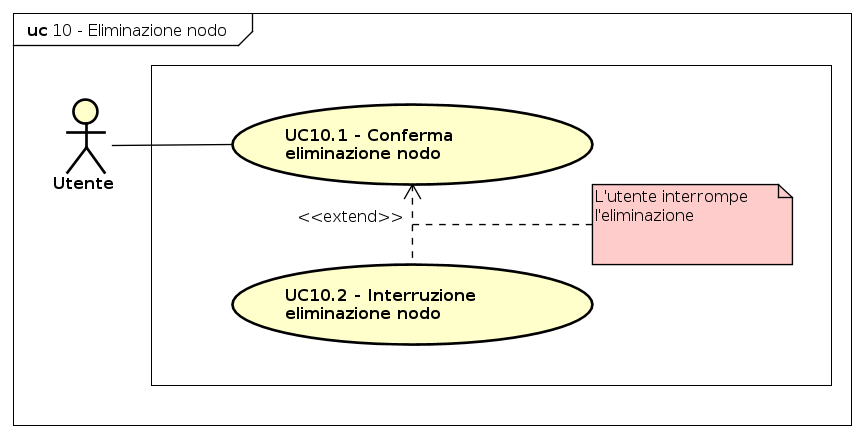
\includegraphics[scale=0.5]{{img/uc10}.png}
\caption{UC10 - Eliminazione nodo}
\end{figure}
\def\arraystretch{1.5}
\rowcolors{2}{D}{P}
\begin{tabularx}{\textwidth}{l|p{0.7\textwidth}}
\rowcolor{I} \multicolumn{2}{c}{\color{white}\textbf{UC10 - Eliminazione nodo}} \\
\toprule
\endhead
\textbf{Attori} & Utente\\
\textbf{Descrizione} & l'utente elimina un nodo\\
\textbf{Pre-condizione} & l'utente ha aperto l'applicazione; è stato inserito almeno un nodo; l'utente ha selezionato un nodo\\
\textbf{Post-condizione} & il nodo è stato eliminato\\
\textbf{Scenario principale} & \vspace{-1.2em}\begin{enumerate}[leftmargin=*,noitemsep,nosep]
\item \nameref{sssec:UC10.1}.
\end{enumerate}\\
\textbf{Scenari alternativi} & \vspace{-1.2em}\begin{itemize}[leftmargin=*,noitemsep,nosep]
\item \nameref{sssec:UC10.2}.
\end{itemize}\\
%\textbf{Generalizzazioni} &  \\
\bottomrule
\end{tabularx}
\subsection{UC10.1 - Conferma eliminazione nodo}
\label{sssec:UC10.1}
\def\arraystretch{1.5}
\rowcolors{2}{D}{P}
\begin{tabularx}{\textwidth}{l|p{0.7\textwidth}}
\rowcolor{I} \multicolumn{2}{c}{\color{white}\textbf{UC10.1 - Conferma eliminazione nodo}} \\
\toprule
\endhead
\textbf{Attori} & Utente\\
\textbf{Descrizione} & l'utente conferma l'eliminazione del nodo\\
\textbf{Pre-condizione} & il sistema offre la possibilità di confermare l'eliminazione del nodo\\
\textbf{Post-condizione} & il nodo è stato eliminato\\
\textbf{Estensioni} & \vspace{-1.2em}\begin{itemize}[leftmargin=*,noitemsep,nosep]
\item \nameref{sssec:UC10.2}.
\end{itemize}\\
%\textbf{Generalizzazioni} &  \\
\bottomrule
\end{tabularx}
\subsection{UC10.2 - Interruzione eliminazione nodo}
\label{sssec:UC10.2}
\def\arraystretch{1.5}
\rowcolors{2}{D}{P}
\begin{tabularx}{\textwidth}{l|p{0.7\textwidth}}
\rowcolor{I} \multicolumn{2}{c}{\color{white}\textbf{UC10.2 - Interruzione eliminazione nodo}} \\
\toprule
\endhead
\textbf{Attori} & Utente\\
\textbf{Descrizione} & l'utente interrompe l'eliminazione del nodo\\
\textbf{Pre-condizione} & il sistema offre la possibilità di confermare l'eliminazione del nodo\\
\textbf{Post-condizione} & il nodo non è stato eliminato\\
%\textbf{Generalizzazioni} &  \\
\bottomrule
\end{tabularx}
\subsection{UC11 - Aggiunta arco}
\label{sssec:UC11}
\begin{figure}[H]
\centering
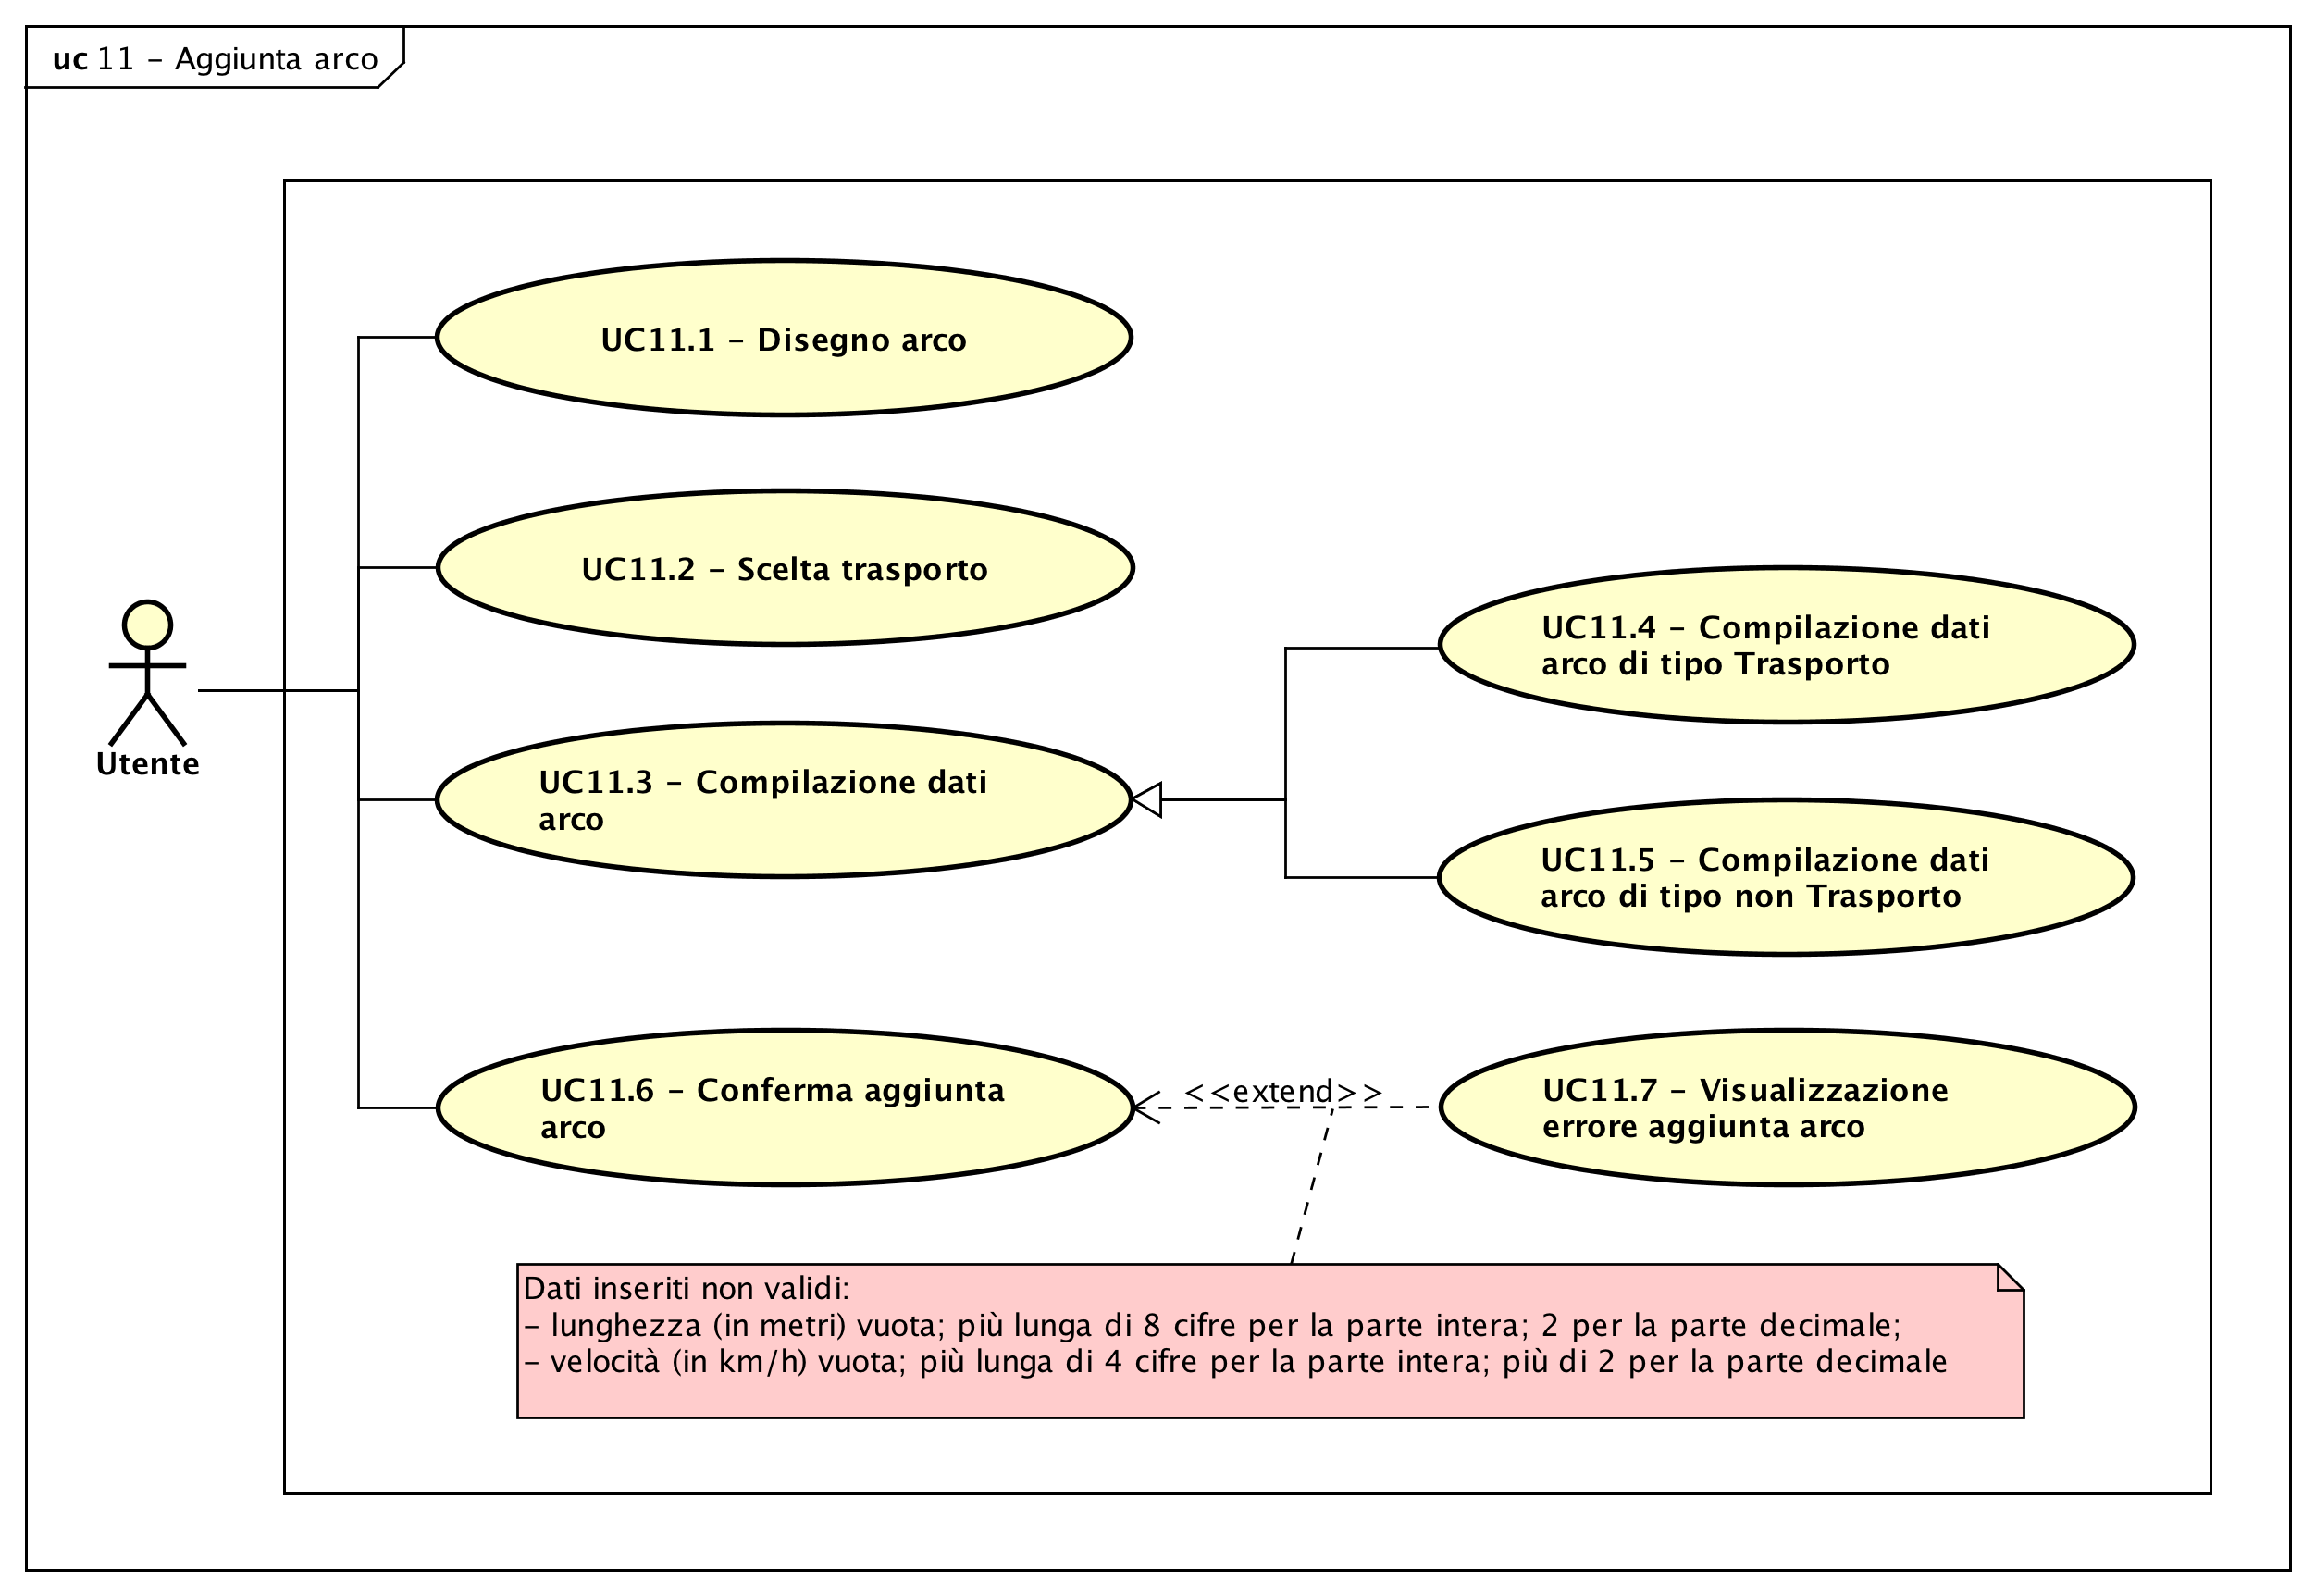
\includegraphics[width=\textwidth]{{img/uc11}.png}
\caption{UC11 - Aggiunta arco}
\end{figure}
\def\arraystretch{1.5}
\rowcolors{2}{D}{P}
\begin{tabularx}{\textwidth}{l|p{0.7\textwidth}}
\rowcolor{I} \multicolumn{2}{c}{\color{white}\textbf{UC11 - Aggiunta arco}} \\
\toprule
\endhead
\textbf{Attori} & Utente\\
\textbf{Descrizione} & l'utente aggiunge un arco\\
\textbf{Pre-condizione} & l'utente ha aperto l'applicazione; è stato inserito almeno un nodo\\
\textbf{Post-condizione} & un nuovo arco è stato aggiunto\\
\textbf{Scenario principale} & \vspace{-1.2em}\begin{enumerate}[leftmargin=*,noitemsep,nosep]
\item \nameref{sssec:UC11.1};
\item \nameref{sssec:UC11.2};
\item \nameref{sssec:UC11.3};
\item \nameref{sssec:UC11.5}.
\end{enumerate}\\
\textbf{Scenari alternativi} & \vspace{-1.2em}\begin{itemize}[leftmargin=*,noitemsep,nosep]
\item \nameref{sssec:UC11.4};
\item \nameref{sssec:UC11.6}.
\end{itemize}\\
%\textbf{Generalizzazioni} &  \\
\bottomrule
\end{tabularx}
\subsection{UC11.1 - Disegno arco}
\label{sssec:UC11.1}
\begin{figure}[H]
\centering
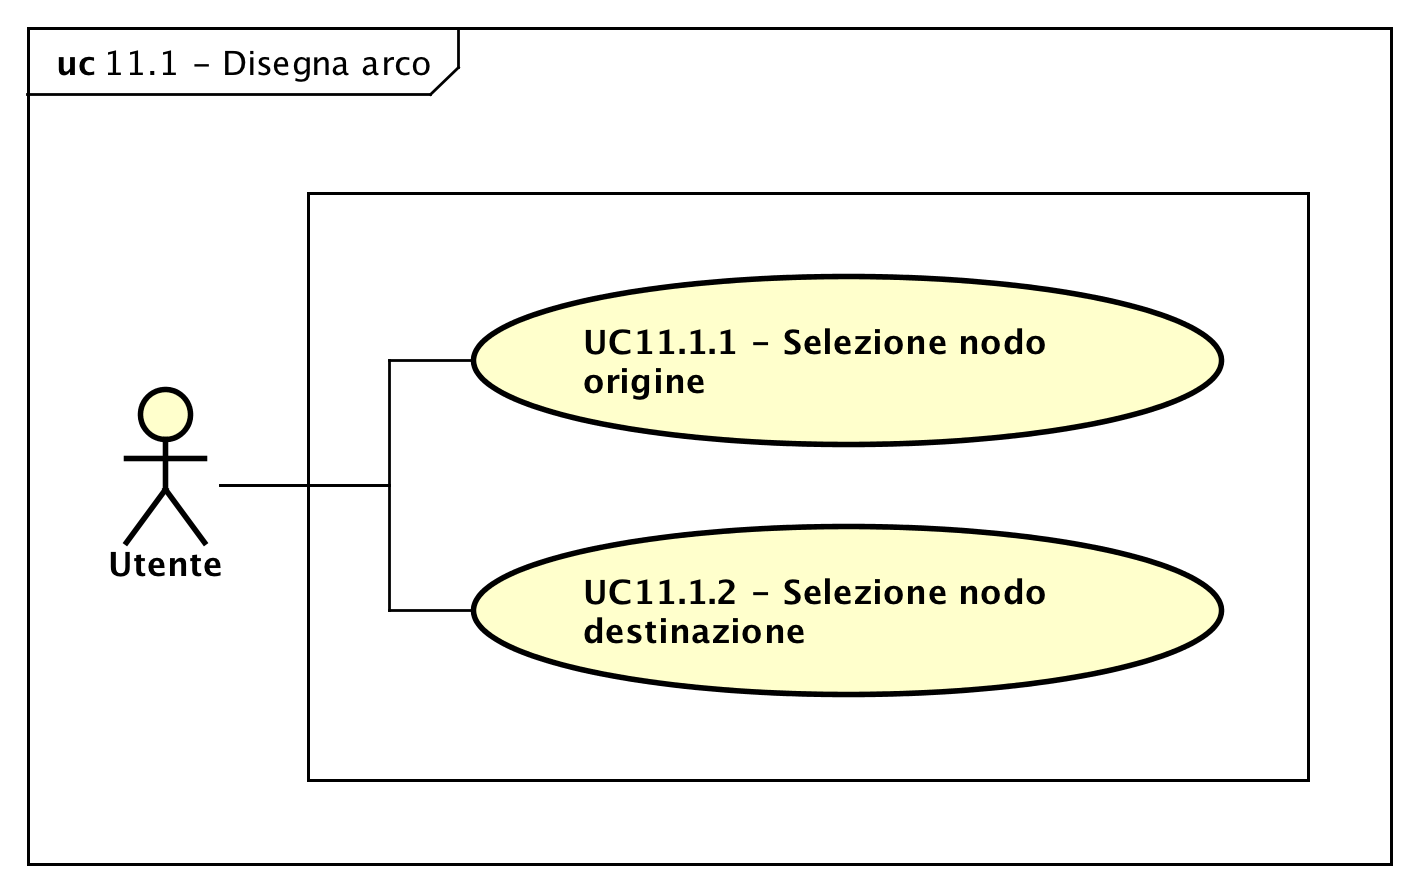
\includegraphics[scale=0.5]{{img/uc11.1}.png}
\caption{UC11.1 - Disegno arco}
\end{figure}
\def\arraystretch{1.5}
\rowcolors{2}{D}{P}
\begin{tabularx}{\textwidth}{l|p{0.7\textwidth}}
\rowcolor{I} \multicolumn{2}{c}{\color{white}\textbf{UC11.1 - Disegno arco}} \\
\toprule
\endhead
\textbf{Attori} & Utente\\
\textbf{Descrizione} & l'utente disegna un arco\\
\textbf{Pre-condizione} & il sistema offre la possibilità di disegnare un arco\\
\textbf{Post-condizione} & un arco è stato disegnato\\
\textbf{Scenario principale} & \vspace{-1.2em}\begin{enumerate}[leftmargin=*,noitemsep,nosep]
\item \nameref{sssec:UC11.1.1};
\item \nameref{sssec:UC11.1.2}.
\end{enumerate}\\
\textbf{Estensioni} & \vspace{-1.2em}\begin{itemize}[leftmargin=*,noitemsep,nosep]
\item \nameref{sssec:UC11.4}.
\end{itemize}\\
%\textbf{Generalizzazioni} &  \\
\bottomrule
\end{tabularx}
\subsection{UC11.1.1 - Selezione nodo di origine}
\label{sssec:UC11.1.1}
\def\arraystretch{1.5}
\rowcolors{2}{D}{P}
\begin{tabularx}{\textwidth}{l|p{0.7\textwidth}}
\rowcolor{I} \multicolumn{2}{c}{\color{white}\textbf{UC11.1.1 - Selezione nodo di origine}} \\
\toprule
\endhead
\textbf{Attori} & Utente\\
\textbf{Descrizione} & l'utente seleziona il nodo di origine dell'arco\\
\textbf{Pre-condizione} & il sistema offre la possibilità di selezionare il nodo di origine\\
\textbf{Post-condizione} & il nodo di origine è stato selezionato\\
%\textbf{Generalizzazioni} &  \\
\bottomrule
\end{tabularx}
\subsection{UC11.1.2 - Selezione nodo di destinazione}
\label{sssec:UC11.1.2}
\def\arraystretch{1.5}
\rowcolors{2}{D}{P}
\begin{tabularx}{\textwidth}{l|p{0.7\textwidth}}
\rowcolor{I} \multicolumn{2}{c}{\color{white}\textbf{UC11.1.2 - Selezione nodo di destinazione}} \\
\toprule
\endhead
\textbf{Attori} & Utente\\
\textbf{Descrizione} & l'utente seleziona il nodo di destinazione dell'arco\\
\textbf{Pre-condizione} & il sistema offre la possibilità di selezionare il nodo di destinazione\\
\textbf{Post-condizione} & il nodo di destinazione è stato selezionato\\
%\textbf{Generalizzazioni} &  \\
\bottomrule
\end{tabularx}
\subsection{UC11.2 - Scelta trasporto}
\label{sssec:UC11.2}
\def\arraystretch{1.5}
\rowcolors{2}{D}{P}
\begin{tabularx}{\textwidth}{l|p{0.7\textwidth}}
\rowcolor{I} \multicolumn{2}{c}{\color{white}\textbf{UC11.2 - Scelta trasporto}} \\
\toprule
\endhead
\textbf{Attori} & Utente\\
\textbf{Descrizione} & l'utente sceglie se l'arco è di tipo trasporto oppure no\\
\textbf{Pre-condizione} & il sistema offre la possibilità di specificare se un arco è di tipo trasporto\\
\textbf{Post-condizione} & l'utente ha scelto se l'arco è di tipo trasporto oppure no\\
\textbf{Estensioni} & \vspace{-1.2em}\begin{itemize}[leftmargin=*,noitemsep,nosep]
\item \nameref{sssec:UC11.4}.
\end{itemize}\\
%\textbf{Generalizzazioni} &  \\
\bottomrule
\end{tabularx}
\subsection{UC11.3 - Compilazione dati arco}
\label{sssec:UC11.3}
\begin{figure}[H]
\centering
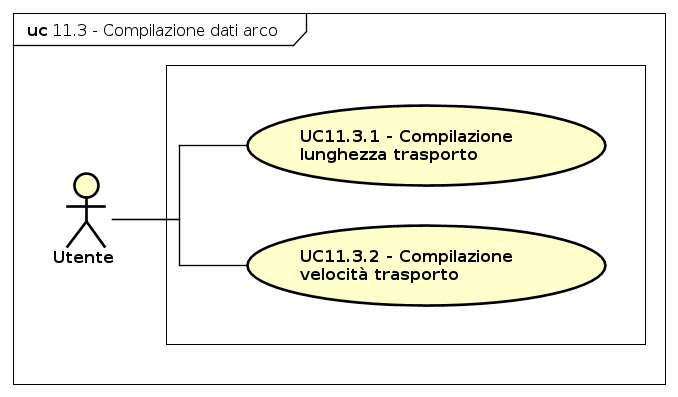
\includegraphics[scale=0.5]{{img/uc11.3}.png}
\caption{UC11.3 - Compilazione dati arco}
\end{figure}
\def\arraystretch{1.5}
\rowcolors{2}{D}{P}
\begin{tabularx}{\textwidth}{l|p{0.7\textwidth}}
\rowcolor{I} \multicolumn{2}{c}{\color{white}\textbf{UC11.3 - Compilazione dati arco}} \\
\toprule
\endhead
\textbf{Attori} & Utente\\
\textbf{Descrizione} & l'utente compila i dati dell'arco\\
\textbf{Pre-condizione} & l'utente ha disegnato l'arco; l'utente ha specificato che l'arco è di tipo trasporto\\
\textbf{Post-condizione} & i dati dell'arco sono stati compilati\\
\textbf{Scenario principale} & \vspace{-1.2em}\begin{enumerate}[leftmargin=*,noitemsep,nosep]
\item \nameref{sssec:UC11.3.1};
\item \nameref{sssec:UC11.3.2}.
\end{enumerate}\\
\textbf{Estensioni} & \vspace{-1.2em}\begin{itemize}[leftmargin=*,noitemsep,nosep]
\item \nameref{sssec:UC11.4}.
\end{itemize}\\
%\textbf{Generalizzazioni} &  \\
\bottomrule
\end{tabularx}
\subsection{UC11.3.1 - Compilazione lunghezza trasporto}
\label{sssec:UC11.3.1}
\def\arraystretch{1.5}
\rowcolors{2}{D}{P}
\begin{tabularx}{\textwidth}{l|p{0.7\textwidth}}
\rowcolor{I} \multicolumn{2}{c}{\color{white}\textbf{UC11.3.1 - Compilazione lunghezza trasporto}} \\
\toprule
\endhead
\textbf{Attori} & Utente\\
\textbf{Descrizione} & l'utente compila il campo relativo alla lunghezza del trasporto\\
\textbf{Pre-condizione} & il sistema offre la possibilità di compilare il campo relativo alla lunghezza del trasporto\\
\textbf{Post-condizione} & il campo relativo alla lunghezza del trasporto è stato compilato\\
%\textbf{Generalizzazioni} &  \\
\bottomrule
\end{tabularx}
\subsection{UC11.3.2 - Compilazione velocità trasporto}
\label{sssec:UC11.3.2}
\def\arraystretch{1.5}
\rowcolors{2}{D}{P}
\begin{tabularx}{\textwidth}{l|p{0.7\textwidth}}
\rowcolor{I} \multicolumn{2}{c}{\color{white}\textbf{UC11.3.2 - Compilazione velocità trasporto}} \\
\toprule
\endhead
\textbf{Attori} & Utente\\
\textbf{Descrizione} & l'utente compila il campo relativo alla velocità del trasporto\\
\textbf{Pre-condizione} & il sistema offre la possibilità di compilare il campo relativo alla velocità del trasporto\\
\textbf{Post-condizione} & il campo relativo alla lunghezza del trasporto è stato compilato\\
%\textbf{Generalizzazioni} &  \\
\bottomrule
\end{tabularx}
\subsection{UC11.4 - Interruzione aggiunta arco}
\label{sssec:UC11.4}
\def\arraystretch{1.5}
\rowcolors{2}{D}{P}
\begin{tabularx}{\textwidth}{l|p{0.7\textwidth}}
\rowcolor{I} \multicolumn{2}{c}{\color{white}\textbf{UC11.4 - Interruzione aggiunta arco}} \\
\toprule
\endhead
\textbf{Attori} & Utente\\
\textbf{Descrizione} & l'utente interrompe l'aggiunta dell'arco\\
\textbf{Pre-condizione} & il sistema offre la possibilità di aggiungere un arco\\
\textbf{Post-condizione} & nessun arco è stato aggiunto\\
%\textbf{Generalizzazioni} &  \\
\bottomrule
\end{tabularx}
\subsection{UC11.5 - Conferma aggiunta arco}
\label{sssec:UC11.5}
\def\arraystretch{1.5}
\rowcolors{2}{D}{P}
\begin{tabularx}{\textwidth}{l|p{0.7\textwidth}}
\rowcolor{I} \multicolumn{2}{c}{\color{white}\textbf{UC11.5 - Conferma aggiunta arco}} \\
\toprule
\endhead
\textbf{Attori} & Utente\\
\textbf{Descrizione} & l'utente conferma l'aggiunta dell'arco\\
\textbf{Pre-condizione} & il sistema offre la possibilità di confermare l'aggiunta dell'arco\\
\textbf{Post-condizione} & un nuovo arco è stato aggiunto\\
\textbf{Estensioni} & \vspace{-1.2em}\begin{itemize}[leftmargin=*,noitemsep,nosep]
\item \nameref{sssec:UC11.6}.
\end{itemize}\\
%\textbf{Generalizzazioni} &  \\
\bottomrule
\end{tabularx}
\subsection{UC11.6 - Visualizzazione errore aggiunta arco}
\label{sssec:UC11.6}
\def\arraystretch{1.5}
\rowcolors{2}{D}{P}
\begin{tabularx}{\textwidth}{l|p{0.7\textwidth}}
\rowcolor{I} \multicolumn{2}{c}{\color{white}\textbf{UC11.6 - Visualizzazione errore aggiunta arco}} \\
\toprule
\endhead
\textbf{Attori} & Utente\\
\textbf{Descrizione} & l'utente visualizza un errore relativo ai dati dell'arco compilati in modo errato\\
\textbf{Pre-condizione} & l'utente sta tentando di inserire un nuovo arco\\
\textbf{Post-condizione} & nessun nuovo arco inserito; l'utente visualizza un errore relativo ai dati dell'arcocompilati in modo errato\\
%\textbf{Generalizzazioni} &  \\
\bottomrule
\end{tabularx}
\subsection{UC12 - Visualizzazione info arco}
\label{sssec:UC12}
\def\arraystretch{1.5}
\rowcolors{2}{D}{P}
\begin{tabularx}{\textwidth}{l|p{0.7\textwidth}}
\rowcolor{I} \multicolumn{2}{c}{\color{white}\textbf{UC12 - Visualizzazione info arco}} \\
\toprule
\endhead
\textbf{Attori} & Utente\\
\textbf{Descrizione} & l'utente seleziona un arco e ne visualizza le informazioni\\
\textbf{Pre-condizione} & l'utente ha aperto l'applicazione, è stato inserito almeno un arco\\
\textbf{Post-condizione} & il sistema mostra le informazioni dell'arco selezionato\\
%\textbf{Generalizzazioni} &  \\
\bottomrule
\end{tabularx}
\subsection{UC13 - Chiusura visualizzazione info arco}
\label{sssec:UC13}
\def\arraystretch{1.5}
\rowcolors{2}{D}{P}
\begin{tabularx}{\textwidth}{l|p{0.7\textwidth}}
\rowcolor{I} \multicolumn{2}{c}{\color{white}\textbf{UC13 - Chiusura visualizzazione info arco}} \\
\toprule
\endhead
\textbf{Attori} & Utente\\
\textbf{Descrizione} & l'utente chiude la visualizzazione delle informazioni di un arco\\
\textbf{Pre-condizione} & l'utente ha visualizzato le informazioni di un arco\\
\textbf{Post-condizione} & è stata chiusa la visualizzazione delle informazioni di un arco\\
%\textbf{Generalizzazioni} &  \\
\bottomrule
\end{tabularx}
\subsection{UC14 - Modifica arco}
\label{sssec:UC14}
\begin{figure}[H]
\centering
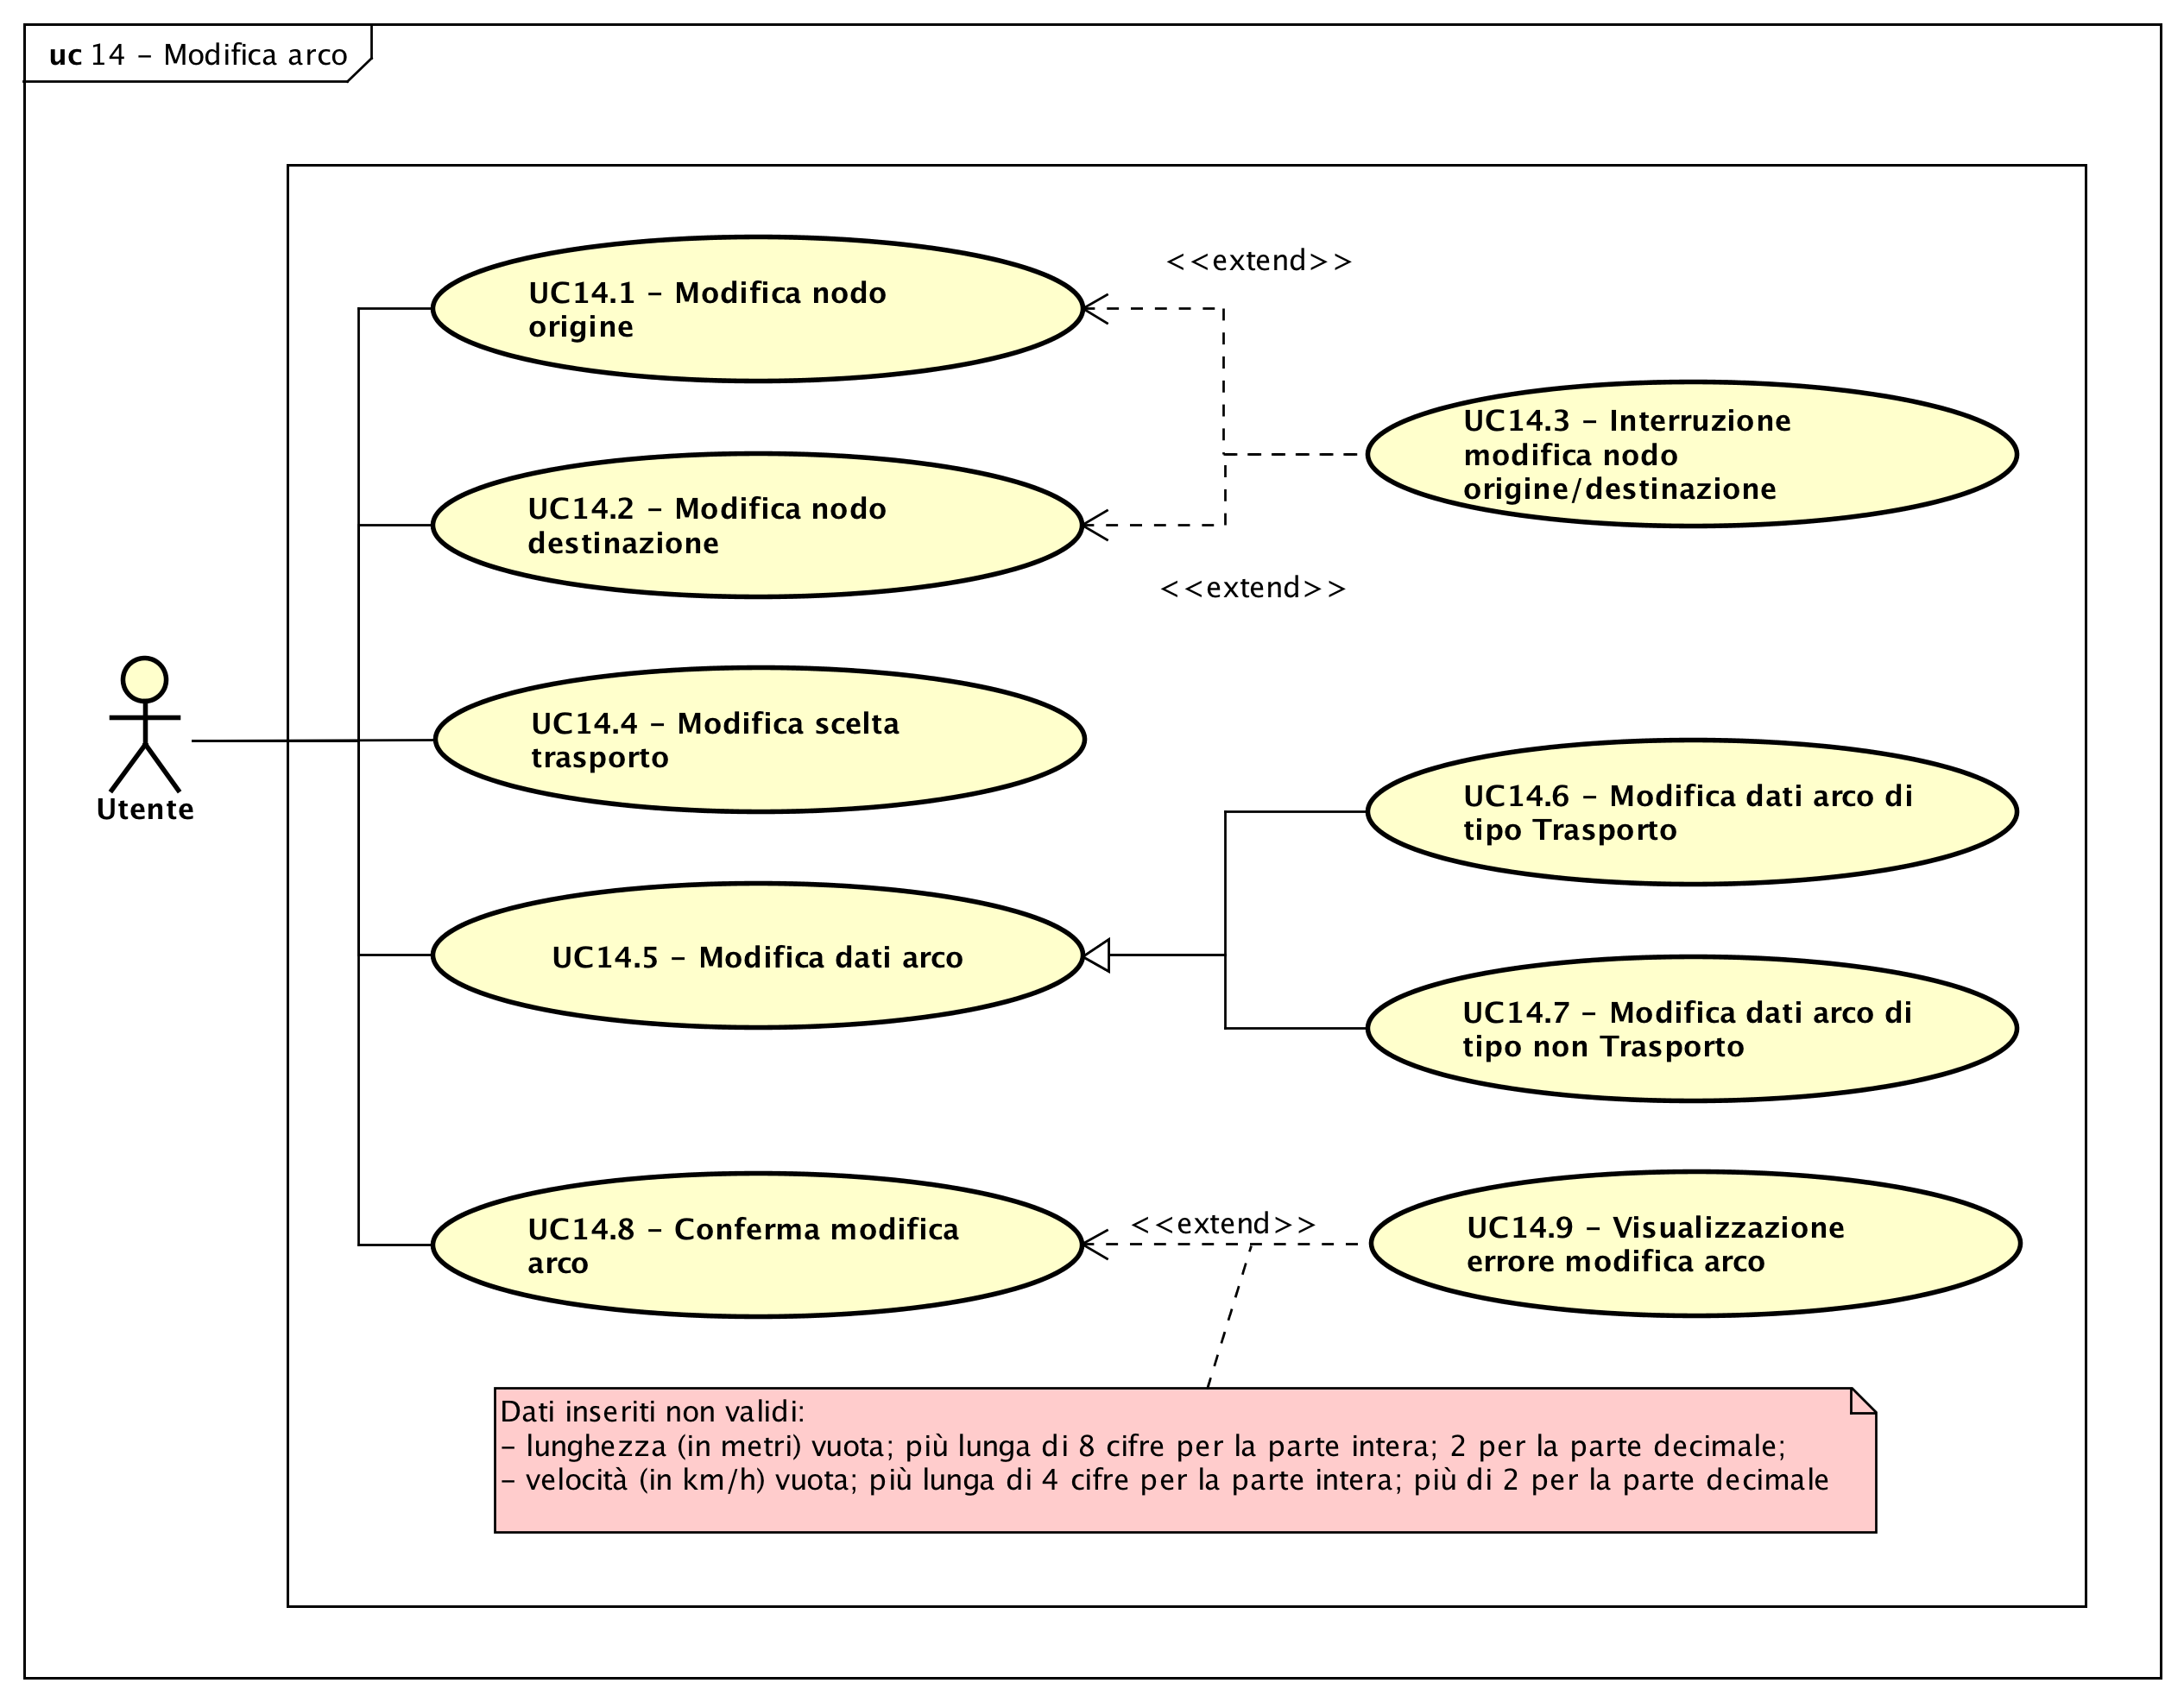
\includegraphics[width=\textwidth]{{img/uc14}.png}
\caption{UC14 - Modifica arco}
\end{figure}
\def\arraystretch{1.5}
\rowcolors{2}{D}{P}
\begin{tabularx}{\textwidth}{l|p{0.7\textwidth}}
\rowcolor{I} \multicolumn{2}{c}{\color{white}\textbf{UC14 - Modifica arco}} \\
\toprule
\endhead
\textbf{Attori} & Utente\\
\textbf{Descrizione} & l'utente modifica l'arco\\
\textbf{Pre-condizione} & l'utente ha aperto l'applicazione; almeno un arco è stato aggiunto; l'utente ha selezionato un arco\\
\textbf{Post-condizione} & l'arco è stato modificato\\
\textbf{Scenario principale} & \vspace{-1.2em}\begin{enumerate}[leftmargin=*,noitemsep,nosep]
\item \nameref{sssec:UC14.1};
\item \nameref{sssec:UC14.2};
\item \nameref{sssec:UC14.4};
\item \nameref{sssec:UC14.5};
\item \nameref{sssec:UC14.7}.
\end{enumerate}\\
\textbf{Scenari alternativi} & \vspace{-1.2em}\begin{itemize}[leftmargin=*,noitemsep,nosep]
\item \nameref{sssec:UC14.3};
\item \nameref{sssec:UC14.6};
\item \nameref{sssec:UC14.8}.
\end{itemize}\\
%\textbf{Generalizzazioni} &  \\
\bottomrule
\end{tabularx}
\subsection{UC14.1 - Modifica nodo origine}
\label{sssec:UC14.1}
\def\arraystretch{1.5}
\rowcolors{2}{D}{P}
\begin{tabularx}{\textwidth}{l|p{0.7\textwidth}}
\rowcolor{I} \multicolumn{2}{c}{\color{white}\textbf{UC14.1 - Modifica nodo origine}} \\
\toprule
\endhead
\textbf{Attori} & Utente\\
\textbf{Descrizione} & l'utente modifica il nodo di origine dell'arco\\
\textbf{Pre-condizione} & il sistema offre la possibilità di modificare il nodo di origine\\
\textbf{Post-condizione} & il nodo di origine è stato modificato\\
\textbf{Estensioni} & \vspace{-1.2em}\begin{itemize}[leftmargin=*,noitemsep,nosep]
\item \nameref{sssec:UC14.3}.
\end{itemize}\\
%\textbf{Generalizzazioni} &  \\
\bottomrule
\end{tabularx}
\subsection{UC14.2 - Modifica nodo destinazione}
\label{sssec:UC14.2}
\def\arraystretch{1.5}
\rowcolors{2}{D}{P}
\begin{tabularx}{\textwidth}{l|p{0.7\textwidth}}
\rowcolor{I} \multicolumn{2}{c}{\color{white}\textbf{UC14.2 - Modifica nodo destinazione}} \\
\toprule
\endhead
\textbf{Attori} & Utente\\
\textbf{Descrizione} & l'utente modifica il nodo di destinazione dell'arco\\
\textbf{Pre-condizione} & il sistema offre la possibilità di modificare il nodo di destinazione\\
\textbf{Post-condizione} & il nodo di destinazione è stato modificato\\
\textbf{Estensioni} & \vspace{-1.2em}\begin{itemize}[leftmargin=*,noitemsep,nosep]
\item \nameref{sssec:UC14.3}.
\end{itemize}\\
%\textbf{Generalizzazioni} &  \\
\bottomrule
\end{tabularx}
\subsection{UC14.3 - Interruzione modifica nodo origine/destinazione}
\label{sssec:UC14.3}
\def\arraystretch{1.5}
\rowcolors{2}{D}{P}
\begin{tabularx}{\textwidth}{l|p{0.7\textwidth}}
\rowcolor{I} \multicolumn{2}{c}{\color{white}\textbf{UC14.3 - Interruzione modifica nodo origine/destinazione}} \\
\toprule
\endhead
\textbf{Attori} & Utente\\
\textbf{Descrizione} & l'utente interrompe la modifica del nodo di origine o di destinazione\\
\textbf{Pre-condizione} & il sistema offre la possibilità di modificare il nodo di origine o di destinazione\\
\textbf{Post-condizione} & il nodo di origine o di destinazione non è stato modificato; l'utente viene riportato alla schermata di modifica\\
%\textbf{Generalizzazioni} &  \\
\bottomrule
\end{tabularx}
\subsection{UC14.4 - Modifica scelta trasporto}
\label{sssec:UC14.4}
\def\arraystretch{1.5}
\rowcolors{2}{D}{P}
\begin{tabularx}{\textwidth}{l|p{0.7\textwidth}}
\rowcolor{I} \multicolumn{2}{c}{\color{white}\textbf{UC14.4 - Modifica scelta trasporto}} \\
\toprule
\endhead
\textbf{Attori} & Utente\\
\textbf{Descrizione} & l'utente modifica la scelta riguardo il trasporto\\
\textbf{Pre-condizione} & il sistema offre la possibilità di modificare la scelta riguardo il trasporto\\
\textbf{Post-condizione} & la scelta riguardo il trasporto è stata modificata\\
%\textbf{Generalizzazioni} &  \\
\bottomrule
\end{tabularx}
\subsection{UC14.5 - Modifica dati arco}
\label{sssec:UC14.5}
\begin{figure}[H]
\centering
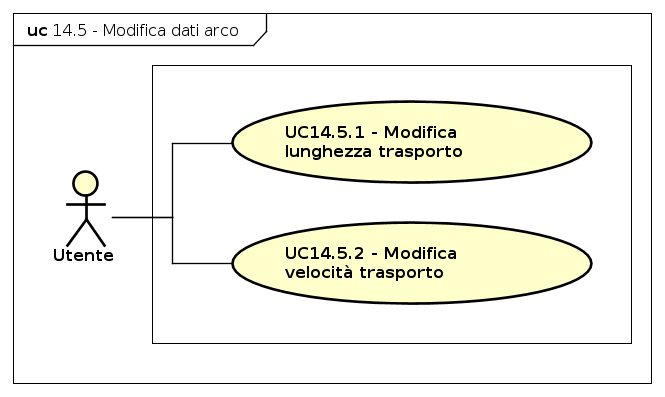
\includegraphics[scale=0.5]{{img/uc14.5}.png}
\caption{UC14.5 - Modifica dati arco}
\end{figure}
\def\arraystretch{1.5}
\rowcolors{2}{D}{P}
\begin{tabularx}{\textwidth}{l|p{0.7\textwidth}}
\rowcolor{I} \multicolumn{2}{c}{\color{white}\textbf{UC14.5 - Modifica dati arco}} \\
\toprule
\endhead
\textbf{Attori} & Utente\\
\textbf{Descrizione} & l'utente modifica i dati dell'arco\\
\textbf{Pre-condizione} & l'utente ha specificato che l'arco è di tipo trasporto\\
\textbf{Post-condizione} & l'utente ha modificato i dati dell'arco\\
\textbf{Scenario principale} & \vspace{-1.2em}\begin{enumerate}[leftmargin=*,noitemsep,nosep]
\item \nameref{sssec:UC14.5.1};
\item \nameref{sssec:UC14.5.2}.
\end{enumerate}\\
\textbf{Estensioni} & \vspace{-1.2em}\begin{itemize}[leftmargin=*,noitemsep,nosep]
\item \nameref{sssec:UC14.6}.
\end{itemize}\\
%\textbf{Generalizzazioni} &  \\
\bottomrule
\end{tabularx}
\subsection{UC14.5.1 - Modifica lunghezza trasporto}
\label{sssec:UC14.5.1}
\def\arraystretch{1.5}
\rowcolors{2}{D}{P}
\begin{tabularx}{\textwidth}{l|p{0.7\textwidth}}
\rowcolor{I} \multicolumn{2}{c}{\color{white}\textbf{UC14.5.1 - Modifica lunghezza trasporto}} \\
\toprule
\endhead
\textbf{Attori} & Utente\\
\textbf{Descrizione} & l'utente modifica la lunghezza del trasporto\\
\textbf{Pre-condizione} & il sistema offre la possibilità di modificare la lunghezza del trasporto; l'utente ha specificato che il nodo è di tipo trasporto\\
\textbf{Post-condizione} & la lunghezza del trasporto è stata modificata\\
%\textbf{Generalizzazioni} &  \\
\bottomrule
\end{tabularx}
\subsection{UC14.5.2 - Modifica velocità trasporto}
\label{sssec:UC14.5.2}
\def\arraystretch{1.5}
\rowcolors{2}{D}{P}
\begin{tabularx}{\textwidth}{l|p{0.7\textwidth}}
\rowcolor{I} \multicolumn{2}{c}{\color{white}\textbf{UC14.5.2 - Modifica velocità trasporto}} \\
\toprule
\endhead
\textbf{Attori} & Utente\\
\textbf{Descrizione} & l'utente modifica la velocità del trasporto\\
\textbf{Pre-condizione} & il sistema offre la possibilità di modificare la velocità del trasporto; l'utente ha specificato che il nodo è di tipo trasporto\\
\textbf{Post-condizione} & la velocità del trasporto è stata modificata\\
%\textbf{Generalizzazioni} &  \\
\bottomrule
\end{tabularx}
\subsection{UC14.6 - Interruzione modifica arco}
\label{sssec:UC14.6}
\def\arraystretch{1.5}
\rowcolors{2}{D}{P}
\begin{tabularx}{\textwidth}{l|p{0.7\textwidth}}
\rowcolor{I} \multicolumn{2}{c}{\color{white}\textbf{UC14.6 - Interruzione modifica arco}} \\
\toprule
\endhead
\textbf{Attori} & Utente\\
\textbf{Descrizione} & l'utente interrompe la modifica dell'arco\\
\textbf{Pre-condizione} & il sistema offre la possibilità di modificare un arco\\
\textbf{Post-condizione} & l'arco non è stato modificato\\
%\textbf{Generalizzazioni} &  \\
\bottomrule
\end{tabularx}
\subsection{UC14.7 - Conferma modifica arco}
\label{sssec:UC14.7}
\def\arraystretch{1.5}
\rowcolors{2}{D}{P}
\begin{tabularx}{\textwidth}{l|p{0.7\textwidth}}
\rowcolor{I} \multicolumn{2}{c}{\color{white}\textbf{UC14.7 - Conferma modifica arco}} \\
\toprule
\endhead
\textbf{Attori} & Utente\\
\textbf{Descrizione} & l'utente conferma la modifica dell'arco\\
\textbf{Pre-condizione} & il sistema offre la possibilità di confermare la modifica dell'arco\\
\textbf{Post-condizione} & l'arco è stato modificato\\
\textbf{Estensioni} & \vspace{-1.2em}\begin{itemize}[leftmargin=*,noitemsep,nosep]
\item \nameref{sssec:UC14.8}.
\end{itemize}\\
%\textbf{Generalizzazioni} &  \\
\bottomrule
\end{tabularx}
\subsection{UC14.8 - Visualizzazione errore modifica arco}
\label{sssec:UC14.8}
\def\arraystretch{1.5}
\rowcolors{2}{D}{P}
\begin{tabularx}{\textwidth}{l|p{0.7\textwidth}}
\rowcolor{I} \multicolumn{2}{c}{\color{white}\textbf{UC14.8 - Visualizzazione errore modifica arco}} \\
\toprule
\endhead
\textbf{Attori} & Utente\\
\textbf{Descrizione} & l'utente visualizza un errore relativo alla modifica dell'arco\\
\textbf{Pre-condizione} & l'utente ha confermato la modifica dell'arco\\
\textbf{Post-condizione} & l'arco non è stato modificato e l'utente visualizza un errore\\
%\textbf{Generalizzazioni} &  \\
\bottomrule
\end{tabularx}
\subsection{UC15 - Eliminazione arco}
\label{sssec:UC15}
\begin{figure}[H]
\centering
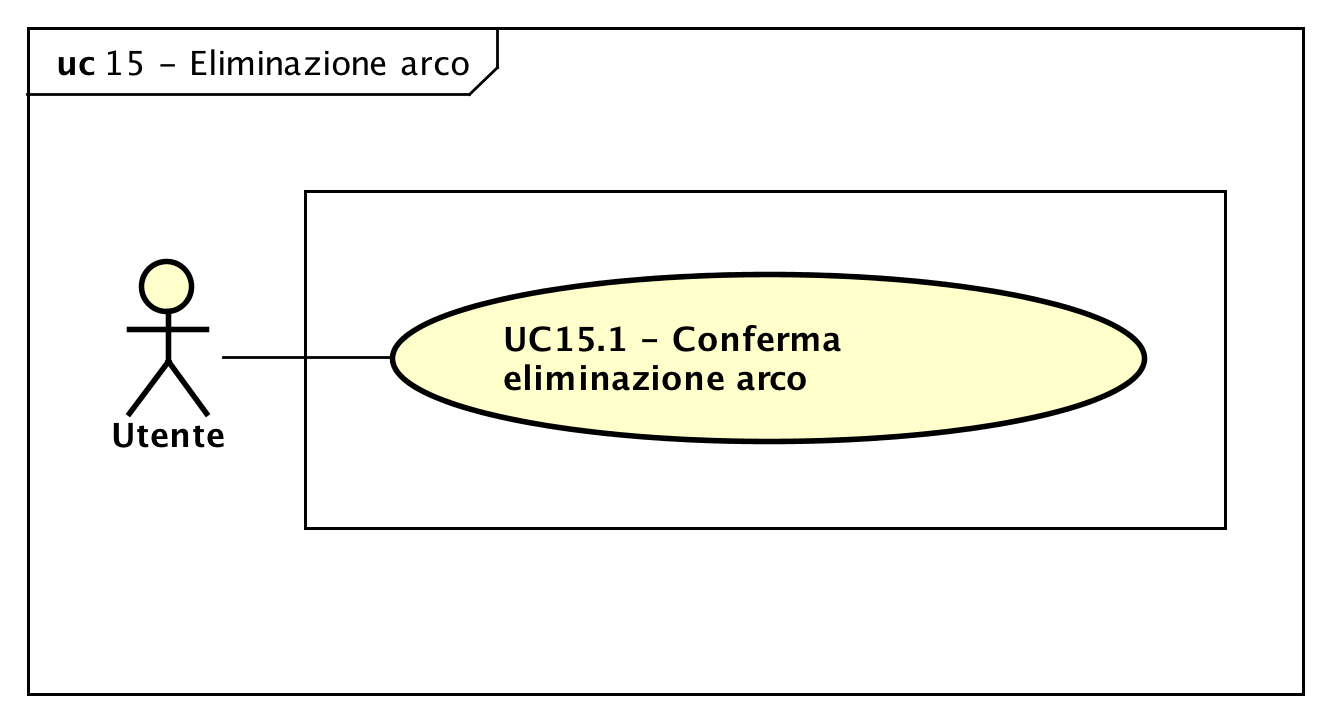
\includegraphics[scale=0.5]{{img/uc15}.png}
\caption{UC15 - Eliminazione arco}
\end{figure}
\def\arraystretch{1.5}
\rowcolors{2}{D}{P}
\begin{tabularx}{\textwidth}{l|p{0.7\textwidth}}
\rowcolor{I} \multicolumn{2}{c}{\color{white}\textbf{UC15 - Eliminazione arco}} \\
\toprule
\endhead
\textbf{Attori} & Utente\\
\textbf{Descrizione} & l'utente elimina un arco\\
\textbf{Pre-condizione} & l'utente ha aperto l'applicazione; è stato inserito almeno un arco; l'utente ha selezionato un arco\\
\textbf{Post-condizione} & l'arco è stato eliminato\\
\textbf{Scenario principale} & \vspace{-1.2em}\begin{enumerate}[leftmargin=*,noitemsep,nosep]
\item \nameref{sssec:UC15.1}.
\end{enumerate}\\
\textbf{Scenari alternativi} & \vspace{-1.2em}\begin{itemize}[leftmargin=*,noitemsep,nosep]
\item \nameref{sssec:UC15.2}.
\end{itemize}\\
%\textbf{Generalizzazioni} &  \\
\bottomrule
\end{tabularx}
\subsection{UC15.1 - Conferma eliminazione arco}
\label{sssec:UC15.1}
\def\arraystretch{1.5}
\rowcolors{2}{D}{P}
\begin{tabularx}{\textwidth}{l|p{0.7\textwidth}}
\rowcolor{I} \multicolumn{2}{c}{\color{white}\textbf{UC15.1 - Conferma eliminazione arco}} \\
\toprule
\endhead
\textbf{Attori} & Utente\\
\textbf{Descrizione} & l'utente conferma l'eliminazione dell'arco\\
\textbf{Pre-condizione} & il sistema offre la possibilità di confermare l'eliminazione dell'arco\\
\textbf{Post-condizione} & l'arco è stato eliminato\\
\textbf{Estensioni} & \vspace{-1.2em}\begin{itemize}[leftmargin=*,noitemsep,nosep]
\item \nameref{sssec:UC15.2}.
\end{itemize}\\
%\textbf{Generalizzazioni} &  \\
\bottomrule
\end{tabularx}
\subsection{UC15.2 - Interruzione eliminazione arco}
\label{sssec:UC15.2}
\def\arraystretch{1.5}
\rowcolors{2}{D}{P}
\begin{tabularx}{\textwidth}{l|p{0.7\textwidth}}
\rowcolor{I} \multicolumn{2}{c}{\color{white}\textbf{UC15.2 - Interruzione eliminazione arco}} \\
\toprule
\endhead
\textbf{Attori} & Utente\\
\textbf{Descrizione} & l'utente interrompe l'eliminazione dell'arco\\
\textbf{Pre-condizione} & il sistema offre la possibilità di confermare l'eliminazione dell'arco\\
\textbf{Post-condizione} & l'arco non è stato eliminato\\
%\textbf{Generalizzazioni} &  \\
\bottomrule
\end{tabularx}
\subsection{UC16 - Aggiunta scenario di danno}
\label{sssec:UC16}
\begin{figure}[H]
\centering
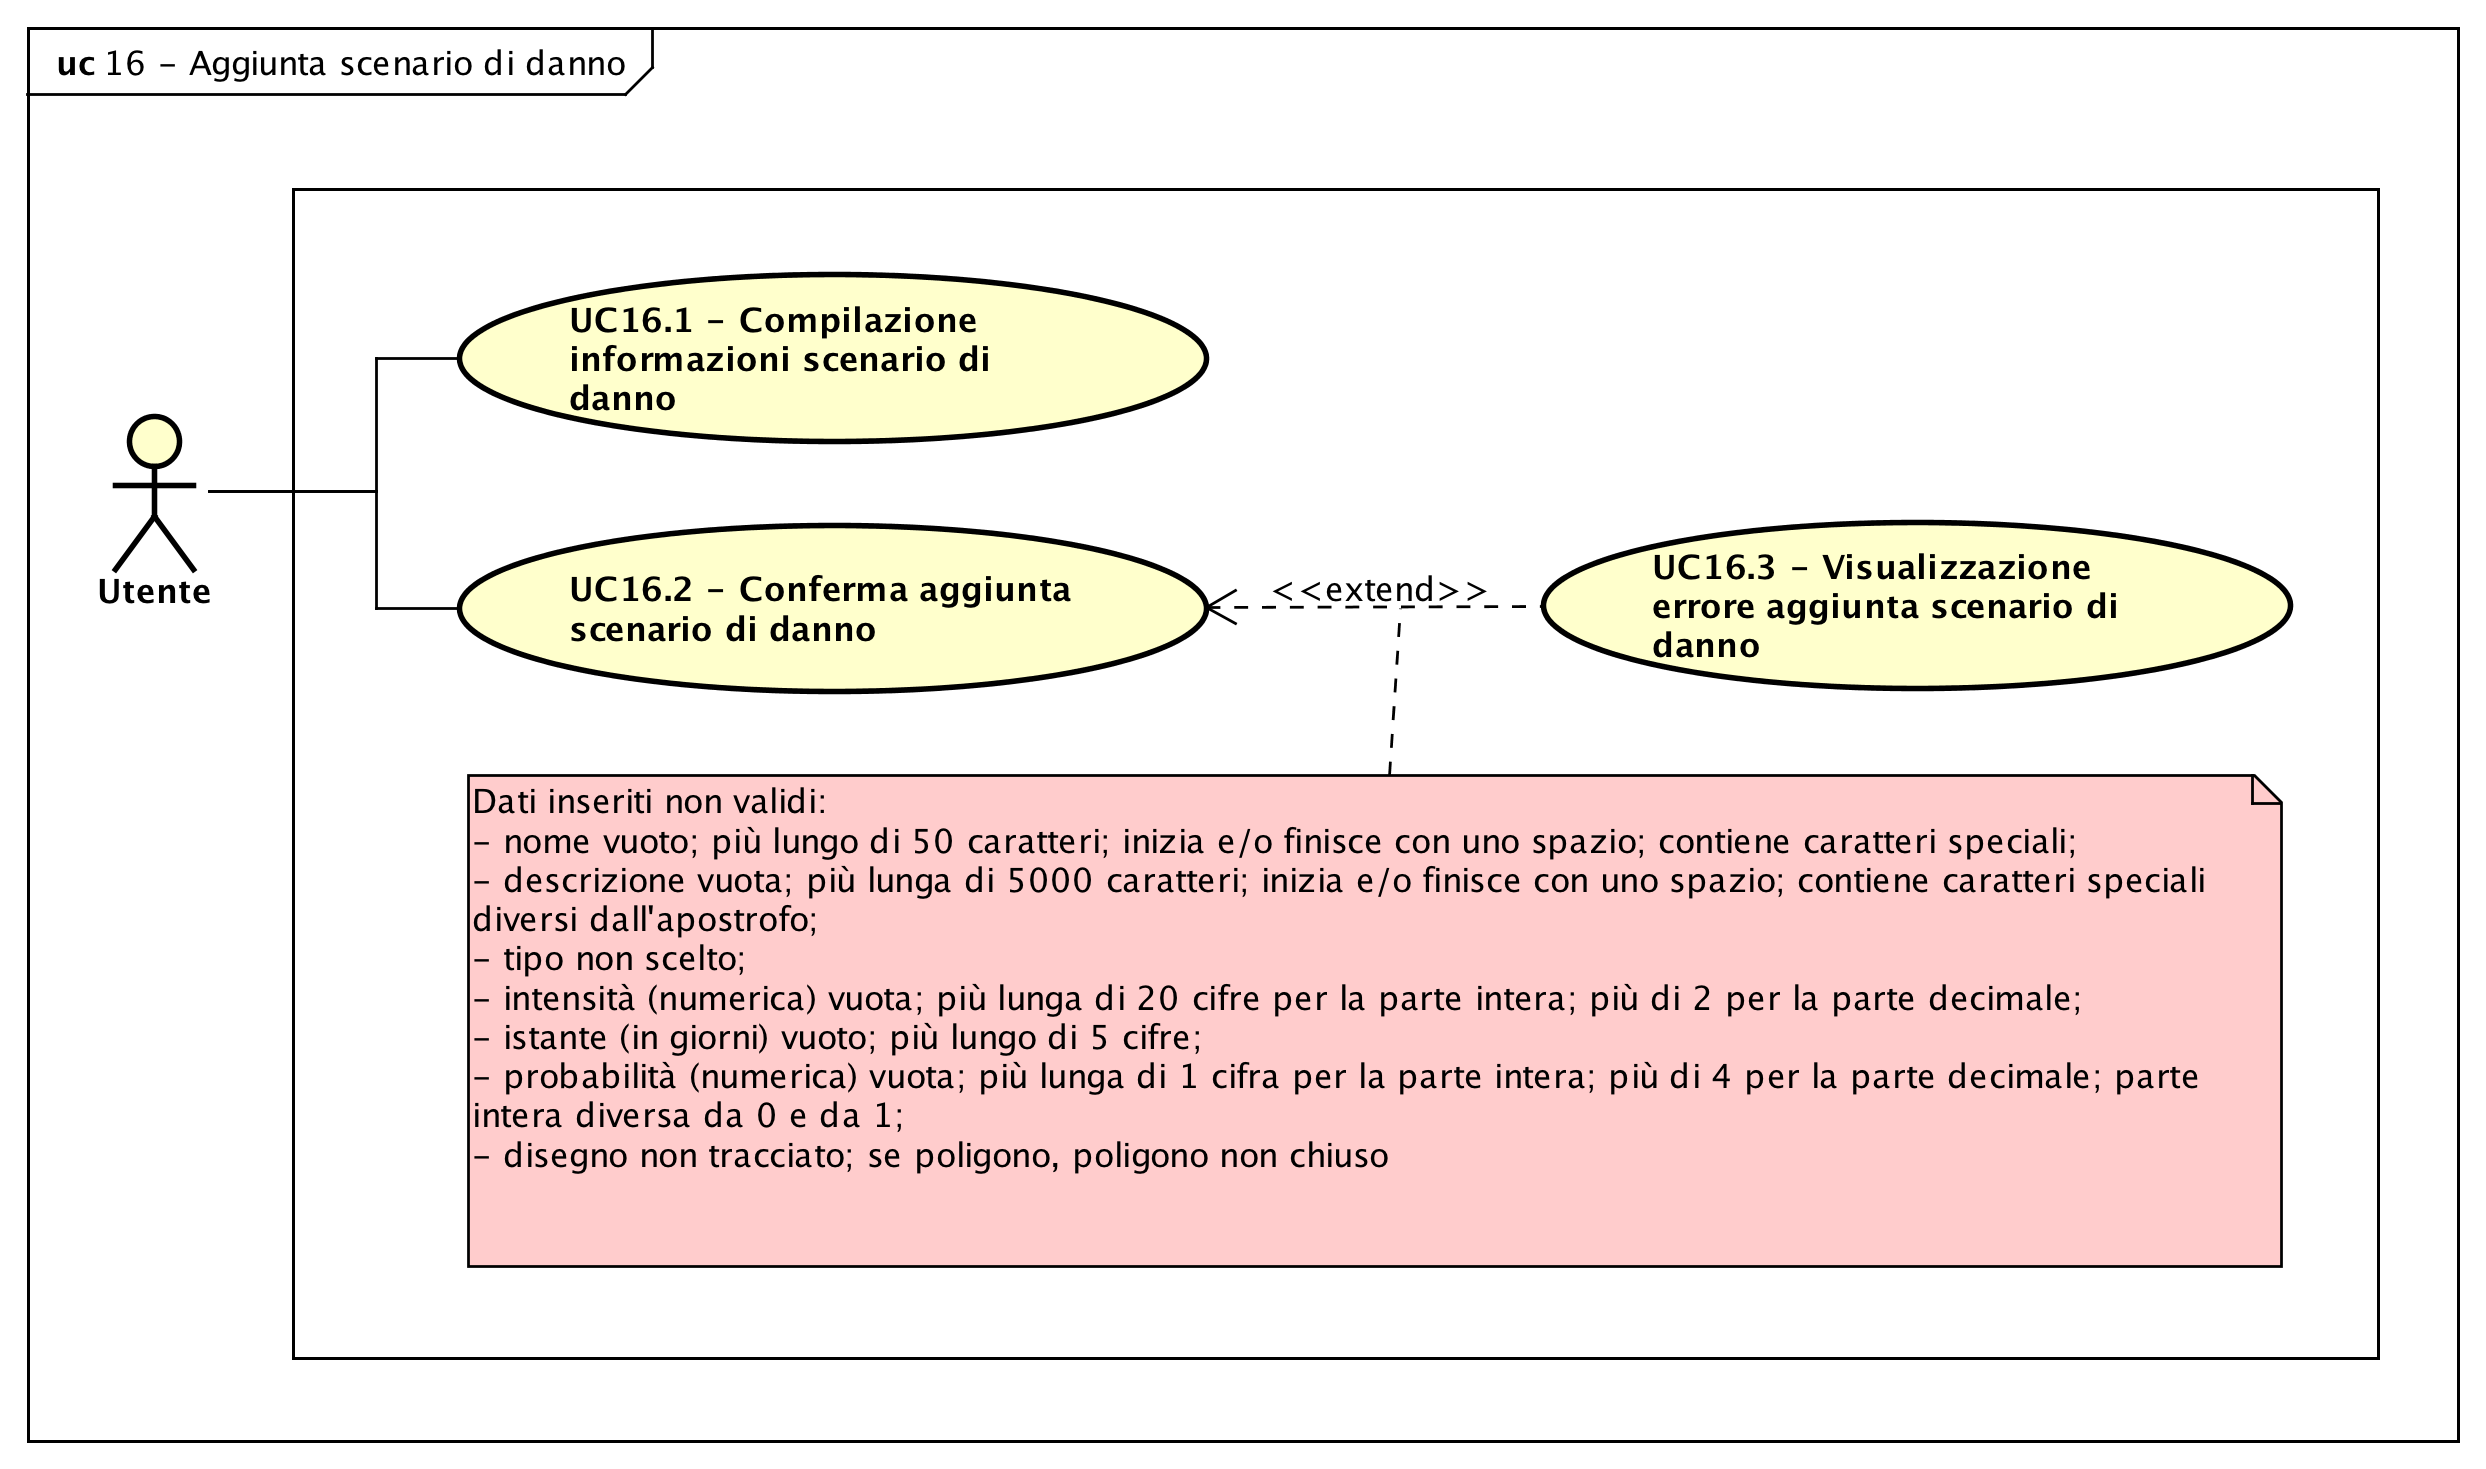
\includegraphics[width=\textwidth]{{img/uc16}.png}
\caption{UC16 - Aggiunta scenario di danno}
\end{figure}
\def\arraystretch{1.5}
\rowcolors{2}{D}{P}
\begin{tabularx}{\textwidth}{l|p{0.7\textwidth}}
\rowcolor{I} \multicolumn{2}{c}{\color{white}\textbf{UC16 - Aggiunta scenario di danno}} \\
\toprule
\endhead
\textbf{Attori} & Utente\\
\textbf{Descrizione} & l'utente aggiunge uno scenario di danno\\
\textbf{Pre-condizione} & l'utente ha aperto l'applicazione\\
\textbf{Post-condizione} & un nuovo scenario di danno è stato aggiunto\\
\textbf{Scenario principale} & \vspace{-1.2em}\begin{enumerate}[leftmargin=*,noitemsep,nosep]
\item \nameref{sssec:UC16.1};
\item \nameref{sssec:UC16.3}.
\end{enumerate}\\
\textbf{Scenari alternativi} & \vspace{-1.2em}\begin{itemize}[leftmargin=*,noitemsep,nosep]
\item \nameref{sssec:UC16.2};
\item \nameref{sssec:UC16.4}.
\end{itemize}\\
%\textbf{Generalizzazioni} &  \\
\bottomrule
\end{tabularx}
\subsection{UC16.1 - Compilazione informazioni scenario di danno}
\label{sssec:UC16.1}
\begin{figure}[H]
\centering
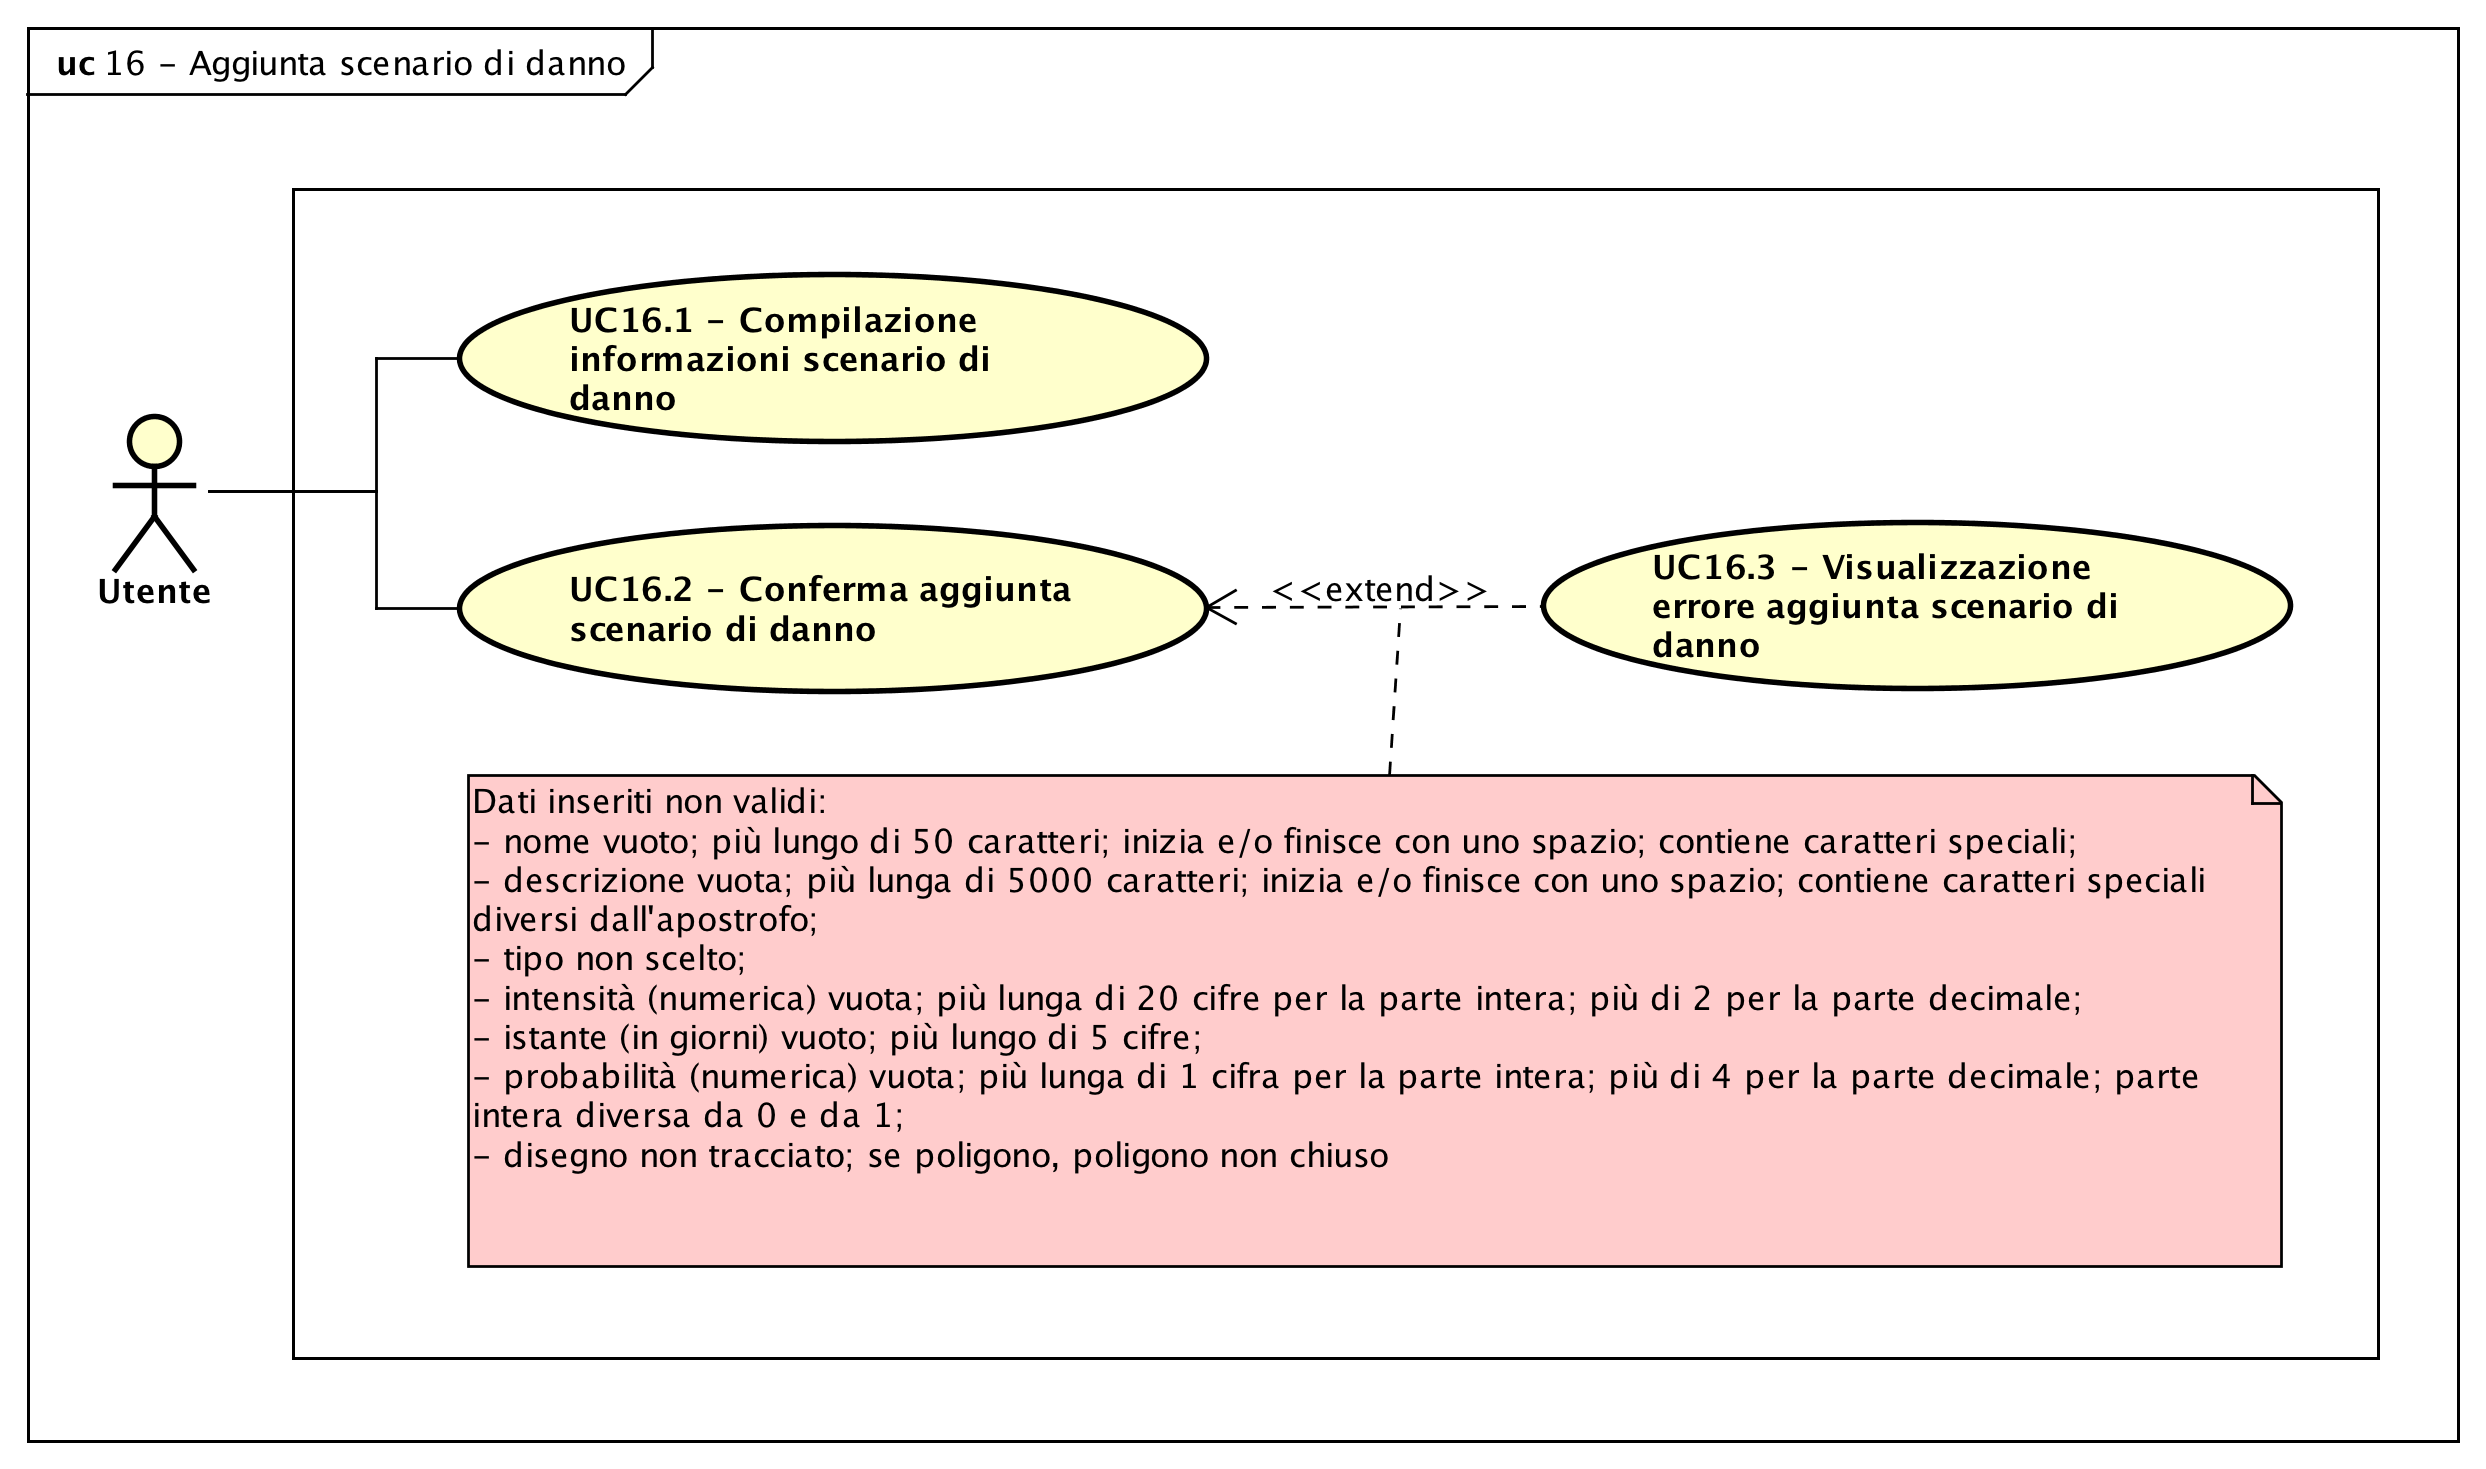
\includegraphics[width=\textwidth]{{img/uc16}.png}
\caption{UC16 - Compilazione informazioni scenario di danno}
\end{figure}
\def\arraystretch{1.5}
\rowcolors{2}{D}{P}
\begin{tabularx}{\textwidth}{l|p{0.7\textwidth}}
\rowcolor{I} \multicolumn{2}{c}{\color{white}\textbf{UC16.1 - Compilazione informazioni scenario di danno}} \\
\toprule
\endhead
\textbf{Attori} & Utente\\
\textbf{Descrizione} & l'utente compila le informazioni dello scenario di danno\\
\textbf{Pre-condizione} & il sistema offre la possbilità di compilare le informazioni dello scenario di danno\\
\textbf{Post-condizione} & le informazioni dello scenario di danno sono state compilate\\
\textbf{Scenario principale} & \vspace{-1.2em}\begin{enumerate}[leftmargin=*,noitemsep,nosep]
\item \nameref{sssec:UC16.1.1};
\item \nameref{sssec:UC16.1.2};
\item \nameref{sssec:UC16.1.3};
\item \nameref{sssec:UC16.1.4};
\item \nameref{sssec:UC16.1.5};
\item \nameref{sssec:UC16.1.6};
\item \nameref{sssec:UC16.1.7};
\end{enumerate}\\
\textbf{Estensioni} & \vspace{-1.2em}\begin{itemize}[leftmargin=*,noitemsep,nosep]
\item \nameref{sssec:UC16.2}.
\end{itemize}\\
\textbf{Scenari alternativi} & \vspace{-1.2em}\begin{itemize}[leftmargin=*,noitemsep,nosep]
\item \nameref{sssec:UC16.1.11}.
\end{itemize}\\
%\textbf{Generalizzazioni} &  \\
\bottomrule
\end{tabularx}
\subsection{UC16.1.1 - Compilazione nome scenario}
\label{sssec:UC16.1.1}
\def\arraystretch{1.5}
\rowcolors{2}{D}{P}
\begin{tabularx}{\textwidth}{l|p{0.7\textwidth}}
\rowcolor{I} \multicolumn{2}{c}{\color{white}\textbf{UC16.1.1 - Compilazione nome scenario}} \\
\toprule
\endhead
\textbf{Attori} & Utente\\
\textbf{Descrizione} & l'utente compila il nome dello scenario\\
\textbf{Pre-condizione} & il sistema offre la possibilità di compilare il nome dello scenario\\
\textbf{Post-condizione} & l'utente ha compilato il nome dello scenario\\
%\textbf{Generalizzazioni} &  \\
\bottomrule
\end{tabularx}
\subsection{UC16.1.10 - Disegno gradiente con linea}
\label{sssec:UC16.1.10}
\def\arraystretch{1.5}
\rowcolors{2}{D}{P}
\begin{tabularx}{\textwidth}{l|p{0.7\textwidth}}
\rowcolor{I} \multicolumn{2}{c}{\color{white}\textbf{UC16.1.10 - Disegno gradiente con linea}} \\
\toprule
\endhead
\textbf{Attori} & Utente\\
\textbf{Descrizione} & l'utente disegna lo scenario di danno mediante gradiente con linea\\
\textbf{Pre-condizione} & il sistema offre la possibilità di disegnare lo scenario\\
\textbf{Post-condizione} & lo scenario è stato disegnato mediante gradiente con linea\\
%\textbf{Generalizzazioni} &  \\
\bottomrule
\end{tabularx}
\subsection{UC16.1.11 - Interruzione disegno scenario}
\label{sssec:UC16.1.11}
\def\arraystretch{1.5}
\rowcolors{2}{D}{P}
\begin{tabularx}{\textwidth}{l|p{0.7\textwidth}}
\rowcolor{I} \multicolumn{2}{c}{\color{white}\textbf{UC16.1.11 - Interruzione disegno scenario}} \\
\toprule
\endhead
\textbf{Attori} & Utente\\
\textbf{Descrizione} & l'utente interrompe il disegno dello scenario\\
\textbf{Pre-condizione} & il sistema offre la possibilità di disegnare lo scenario\\
\textbf{Post-condizione} & lo scenario non è stato disegnato; l'utente viene riportato sulla schermata di inserimento\\
%\textbf{Generalizzazioni} &  \\
\bottomrule
\end{tabularx}
\subsection{UC16.1.2 - Compilazione descrizione scenario}
\label{sssec:UC16.1.2}
\def\arraystretch{1.5}
\rowcolors{2}{D}{P}
\begin{tabularx}{\textwidth}{l|p{0.7\textwidth}}
\rowcolor{I} \multicolumn{2}{c}{\color{white}\textbf{UC16.1.2 - Compilazione descrizione scenario}} \\
\toprule
\endhead
\textbf{Attori} & Utente\\
\textbf{Descrizione} & l'utente compila la descrizione dello scenario\\
\textbf{Pre-condizione} & il sistema offre la possibilità di compilare la descrizione dello scenario\\
\textbf{Post-condizione} & l'utente ha compilato la descrizione dello scenario\\
%\textbf{Generalizzazioni} &  \\
\bottomrule
\end{tabularx}
\subsection{UC16.1.3 - Scelta tipo scenario}
\label{sssec:UC16.1.3}
\def\arraystretch{1.5}
\rowcolors{2}{D}{P}
\begin{tabularx}{\textwidth}{l|p{0.7\textwidth}}
\rowcolor{I} \multicolumn{2}{c}{\color{white}\textbf{UC16.1.3 - Scelta tipo scenario}} \\
\toprule
\endhead
\textbf{Attori} & Utente\\
\textbf{Descrizione} & l'utente sceglie il tipo di scenario\\
\textbf{Pre-condizione} & il sistema offre la possibilità di scegliere il tipo di scenario\\
\textbf{Post-condizione} & il tipo di scenario è stato scelto\\
%\textbf{Generalizzazioni} &  \\
\bottomrule
\end{tabularx}
\subsection{UC16.1.4 - Compilazione intensità scenario}
\label{sssec:UC16.1.4}
\def\arraystretch{1.5}
\rowcolors{2}{D}{P}
\begin{tabularx}{\textwidth}{l|p{0.7\textwidth}}
\rowcolor{I} \multicolumn{2}{c}{\color{white}\textbf{UC16.1.4 - Compilazione intensità scenario}} \\
\toprule
\endhead
\textbf{Attori} & Utente\\
\textbf{Descrizione} & l'utente compila l'intensità dello scenario\\
\textbf{Pre-condizione} & il sistema offre la possibilità di compilare l'intensità dello scenario\\
\textbf{Post-condizione} & l'utente ha compilato l'intensità dello scenario\\
%\textbf{Generalizzazioni} &  \\
\bottomrule
\end{tabularx}
\subsection{UC16.1.5 - Compilazione istante dell'evento scenario}
\label{sssec:UC16.1.5}
\def\arraystretch{1.5}
\rowcolors{2}{D}{P}
\begin{tabularx}{\textwidth}{l|p{0.7\textwidth}}
\rowcolor{I} \multicolumn{2}{c}{\color{white}\textbf{UC16.1.5 - Compilazione istante dell'evento scenario}} \\
\toprule
\endhead
\textbf{Attori} & Utente\\
\textbf{Descrizione} & l'utente compila l'istante dell'evento dello scenario\\
\textbf{Pre-condizione} & il sistema offre la possibilità di compilare l'istante dell'evento dello scenario\\
\textbf{Post-condizione} & l'istante dell'evento dello scenario è stato compilato\\
%\textbf{Generalizzazioni} &  \\
\bottomrule
\end{tabularx}
\subsection{UC16.1.6 - Compilazione probabilità dell'evento scenario}
\label{sssec:UC16.1.6}
\def\arraystretch{1.5}
\rowcolors{2}{D}{P}
\begin{tabularx}{\textwidth}{l|p{0.7\textwidth}}
\rowcolor{I} \multicolumn{2}{c}{\color{white}\textbf{UC16.1.6 - Compilazione probabilità dell'evento scenario}} \\
\toprule
\endhead
\textbf{Attori} & Utente\\
\textbf{Descrizione} & l'utente compila la probabilità dell'evento dello scenario\\
\textbf{Pre-condizione} & il sistema offre la possibilità di compilare la probabilità dell'evento dello scenario\\
\textbf{Post-condizione} & la probabilità dell'evento dello scenario è stata compilata\\
%\textbf{Generalizzazioni} &  \\
\bottomrule
\end{tabularx}
\subsection{UC16.1.7 - Disegno scenario}
\label{sssec:UC16.1.7}
\def\arraystretch{1.5}
\rowcolors{2}{D}{P}
\begin{tabularx}{\textwidth}{l|p{0.7\textwidth}}
\rowcolor{I} \multicolumn{2}{c}{\color{white}\textbf{UC16.1.7 - Disegno scenario}} \\
\toprule
\endhead
\textbf{Attori} & Utente\\
\textbf{Descrizione} & l'utente disegna lo scenario di danno\\
\textbf{Pre-condizione} & il sistema offre la possibilità di disegnare lo scenario di danno\\
\textbf{Post-condizione} & lo scenario di danno è stato disegnato\\
\textbf{Estensioni} & \vspace{-1.2em}\begin{itemize}[leftmargin=*,noitemsep,nosep]
\item \nameref{sssec:UC16.1.11}.
\end{itemize}\\
\textbf{Generalizzazioni} & \vspace{-1.2em}\begin{itemize}[leftmargin=*,noitemsep,nosep]
	\item \nameref{sssec:UC16.1.8}; 
	\item \nameref{sssec:UC16.1.9}; 
	\item \nameref{sssec:UC16.1.10}.
	\end{itemize} \\
\bottomrule
\end{tabularx}
\subsection{UC16.1.8 - Disegno poligono}
\label{sssec:UC16.1.8}
\def\arraystretch{1.5}
\rowcolors{2}{D}{P}
\begin{tabularx}{\textwidth}{l|p{0.7\textwidth}}
\rowcolor{I} \multicolumn{2}{c}{\color{white}\textbf{UC16.1.8 - Disegno poligono}} \\
\toprule
\endhead
\textbf{Attori} & Utente\\
\textbf{Descrizione} & l'utente disegna lo scenario mediante poligono\\
\textbf{Pre-condizione} & il sistema offre la possibilità di disegnare lo scenario\\
\textbf{Post-condizione} & lo scenario è stato disegnato mediante poligono\\
%\textbf{Generalizzazioni} &  \\
\bottomrule
\end{tabularx}
\subsection{UC16.1.9 - Disegno gradiente radiale}
\label{sssec:UC16.1.9}
\def\arraystretch{1.5}
\rowcolors{2}{D}{P}
\begin{tabularx}{\textwidth}{l|p{0.7\textwidth}}
\rowcolor{I} \multicolumn{2}{c}{\color{white}\textbf{UC16.1.9 - Disegno gradiente radiale}} \\
\toprule
\endhead
\textbf{Attori} & Utente\\
\textbf{Descrizione} & l'utente disegna lo scenario di danno mediante gradiente radiale\\
\textbf{Pre-condizione} & il sistema offre la possibilità di disegnare lo scenario\\
\textbf{Post-condizione} & lo scenario è stato disegnato mediante gradiente radiale\\
%\textbf{Generalizzazioni} &  \\
\bottomrule
\end{tabularx}
\subsection{UC16.2 - Interruzione aggiunta scenario di danno}
\label{sssec:UC16.2}
\def\arraystretch{1.5}
\rowcolors{2}{D}{P}
\begin{tabularx}{\textwidth}{l|p{0.7\textwidth}}
\rowcolor{I} \multicolumn{2}{c}{\color{white}\textbf{UC16.2 - Interruzione aggiunta scenario di danno}} \\
\toprule
\endhead
\textbf{Attori} & Utente\\
\textbf{Descrizione} & l'utente interrompe l'aggiunta dello scenario di danno\\
\textbf{Pre-condizione} & il sistema offre la possibilità di aggiungere uno scenario di danno\\
\textbf{Post-condizione} & nessuno scenario è stato aggiunto\\
%\textbf{Generalizzazioni} &  \\
\bottomrule
\end{tabularx}
\subsection{UC16.3 - Conferma aggiunta scenario di danno}
\label{sssec:UC16.3}
\def\arraystretch{1.5}
\rowcolors{2}{D}{P}
\begin{tabularx}{\textwidth}{l|p{0.7\textwidth}}
\rowcolor{I} \multicolumn{2}{c}{\color{white}\textbf{UC16.3 - Conferma aggiunta scenario di danno}} \\
\toprule
\endhead
\textbf{Attori} & Utente\\
\textbf{Descrizione} & l'utente conferma l'aggiunta dello scenario di danno\\
\textbf{Pre-condizione} & il sistema offre la possibilità di confermare l'aggiunta dello scenario di danno\\
\textbf{Post-condizione} & un nuovo scenario di danno è stato aggiunto\\
\textbf{Estensioni} & \vspace{-1.2em}\begin{itemize}[leftmargin=*,noitemsep,nosep]
\item \nameref{sssec:UC16.4}.
\end{itemize}\\
%\textbf{Generalizzazioni} &  \\
\bottomrule
\end{tabularx}
\subsection{UC16.4 - Visualizzazione errore aggiunta scenario di danno}
\label{sssec:UC16.4}
\def\arraystretch{1.5}
\rowcolors{2}{D}{P}
\begin{tabularx}{\textwidth}{l|p{0.7\textwidth}}
\rowcolor{I} \multicolumn{2}{c}{\color{white}\textbf{UC16.4 - Visualizzazione errore aggiunta scenario di danno}} \\
\toprule
\endhead
\textbf{Attori} & Utente\\
\textbf{Descrizione} & l'utente visualizza un errore relativo ai dati dello scenario di danno compilati in modo errato\\
\textbf{Pre-condizione} & l'utente sta tentando di inserire un nuovo scenario di danno\\
\textbf{Post-condizione} & nessun nuovo asset inserito; l'utente visualizza un errore relativo ai dati dello scenario di danno compilati in modo errato\\
%\textbf{Generalizzazioni} &  \\
\bottomrule
\end{tabularx}
\subsection{UC17 - Scelta visualizzazione scenario di danno}
\label{sssec:UC17}
\def\arraystretch{1.5}
\rowcolors{2}{D}{P}
\begin{tabularx}{\textwidth}{l|p{0.7\textwidth}}
\rowcolor{I} \multicolumn{2}{c}{\color{white}\textbf{UC17 - Scelta visualizzazione scenario di danno}} \\
\toprule
\endhead
\textbf{Attori} & Utente\\
\textbf{Descrizione} & l'utente sceglie quale scenario di danno visualizzare\\
\textbf{Pre-condizione} & l'utente ha aperto l'applicazione; almeno uno scenario di danno è stato inserito\\
\textbf{Post-condizione} & l'utente visualizza lo scenario di danno sulla mappa\\
%\textbf{Generalizzazioni} &  \\
\bottomrule
\end{tabularx}
\subsection{UC18 - Chiusura visualizzazione scenario di danno}
\label{sssec:UC18}
\def\arraystretch{1.5}
\rowcolors{2}{D}{P}
\begin{tabularx}{\textwidth}{l|p{0.7\textwidth}}
\rowcolor{I} \multicolumn{2}{c}{\color{white}\textbf{UC18 - Chiusura visualizzazione scenario di danno}} \\
\toprule
\endhead
\textbf{Attori} & Utente\\
\textbf{Descrizione} & l'utente chiude la visualizzazione dello scenario di danno\\
\textbf{Pre-condizione} & l'utente ha aperto l'applicazione; uno scenario di danno è visualizzato sulla mappa\\
\textbf{Post-condizione} & lo scenario di danno non è più visualizzato sulla mappa\\
%\textbf{Generalizzazioni} &  \\
\bottomrule
\end{tabularx}
\subsection{UC19 - Modifica scenario di danno}
\label{sssec:UC19}
\begin{figure}[H]
\centering
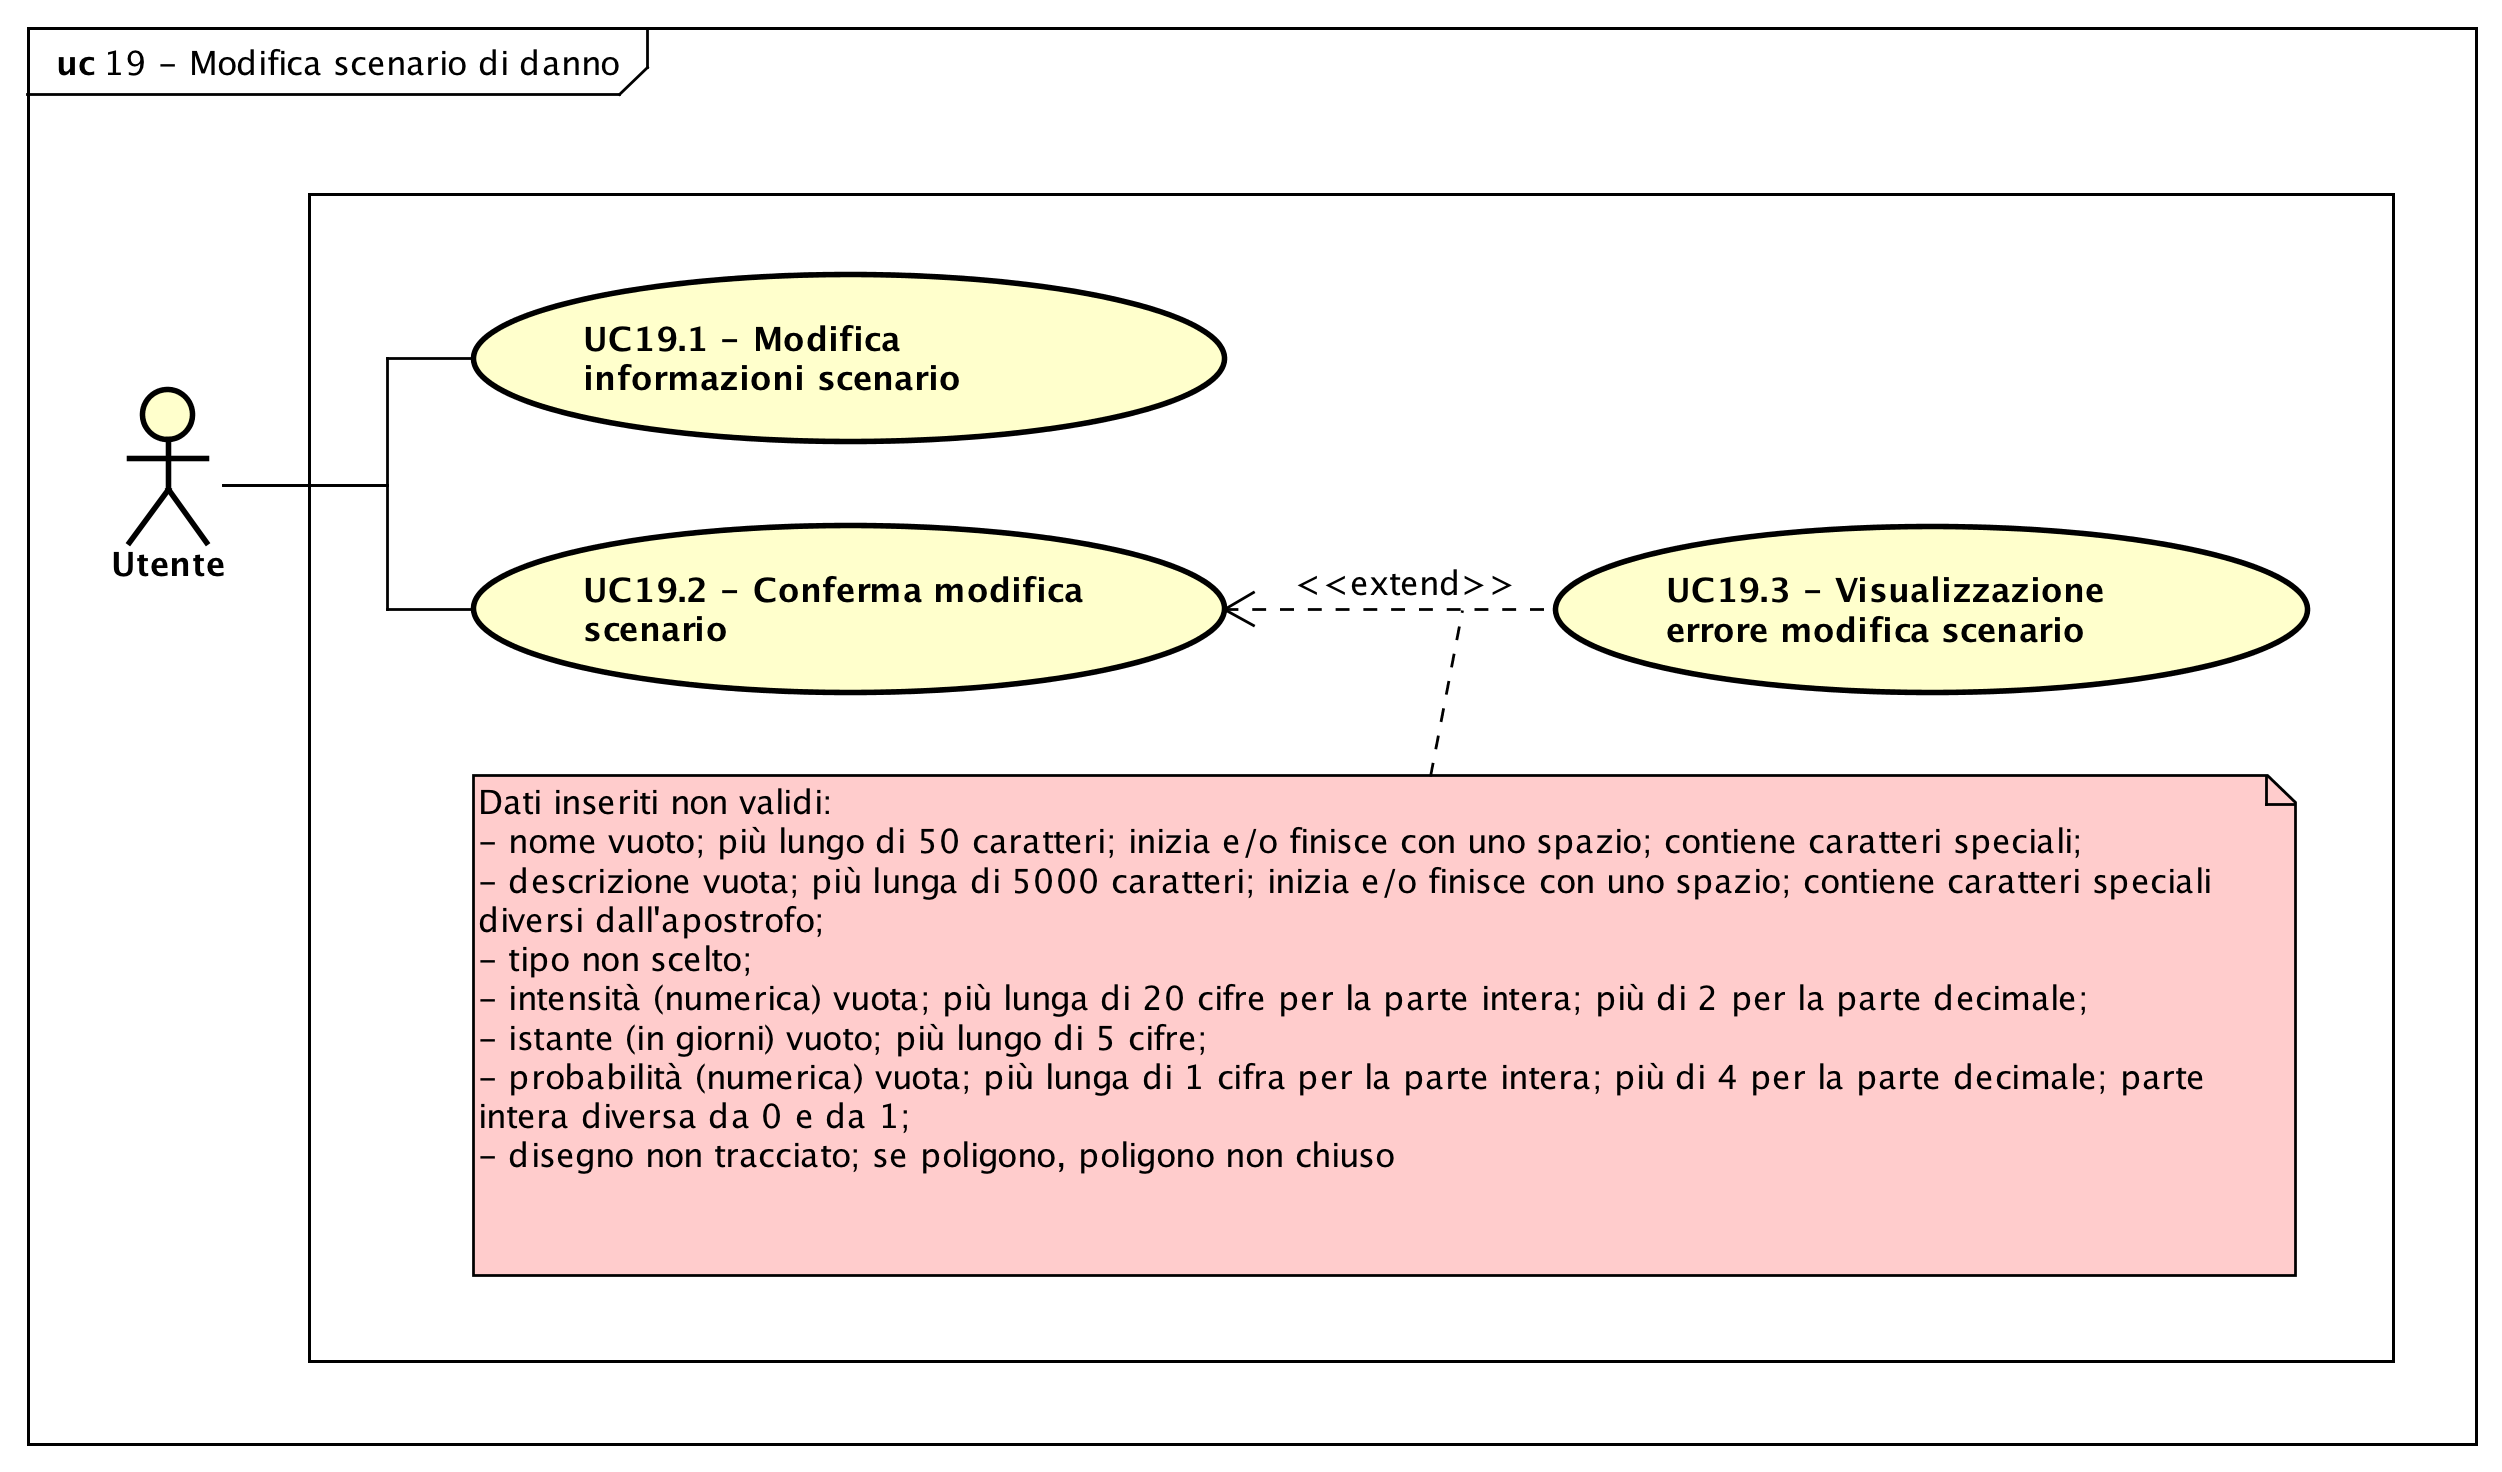
\includegraphics[width=\textwidth]{{img/uc19}.png}
\caption{UC4 - Modifica scenario di danno}
\end{figure}
\def\arraystretch{1.5}
\rowcolors{2}{D}{P}
\begin{tabularx}{\textwidth}{l|p{0.7\textwidth}}
\rowcolor{I} \multicolumn{2}{c}{\color{white}\textbf{UC19 - Modifica scenario di danno}} \\
\toprule
\endhead
\textbf{Attori} & Utente\\
\textbf{Descrizione} & l'utente modifica lo scenario di danno\\
\textbf{Pre-condizione} & l'utente ha aperto l'applicazione; almeno uno scenario di danno è stato aggiunto; l'utente ha selezionato uno scenario di danno\\
\textbf{Post-condizione} & lo scenario di danno è stato modificato\\
\textbf{Scenario principale} & \vspace{-1.2em}\begin{enumerate}[leftmargin=*,noitemsep,nosep]
\item \nameref{sssec:UC19.1};
\item \nameref{sssec:UC19.3};
\item \nameref{sssec:UC19.4}.
\end{enumerate}\\
\textbf{Scenari alternativi} & \vspace{-1.2em}\begin{itemize}[leftmargin=*,noitemsep,nosep]
\item \nameref{sssec:UC19.2}.
\end{itemize}\\
%\textbf{Generalizzazioni} &  \\
\bottomrule
\end{tabularx}
\subsection{UC19.1 - Modifica informazioni scenario}
\label{sssec:UC19.1}
\begin{figure}[H]
\centering
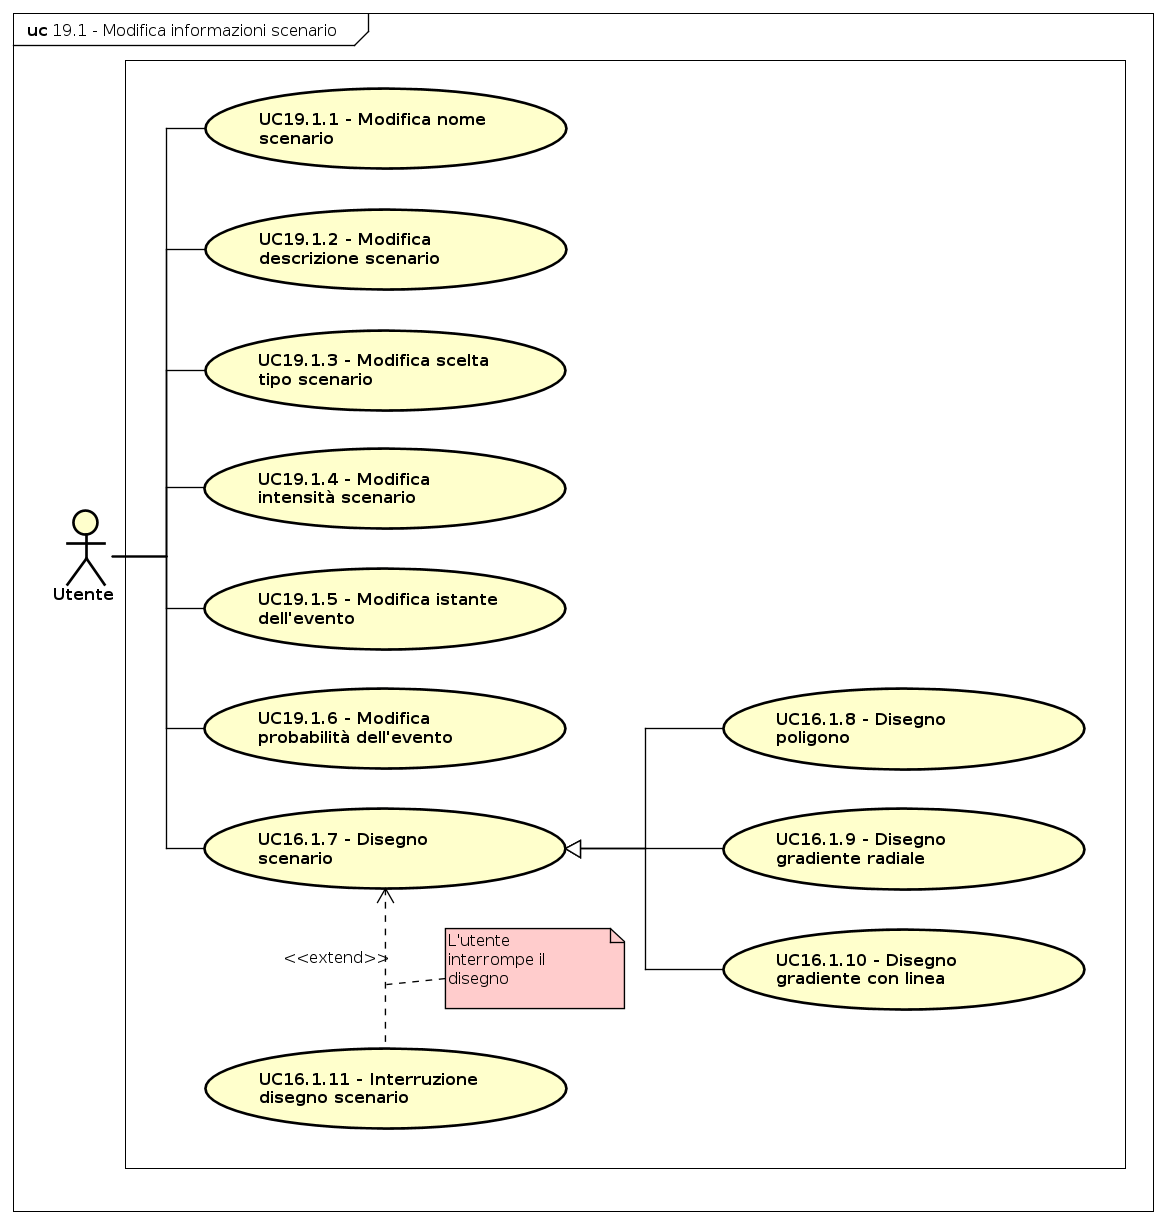
\includegraphics[width=\textwidth]{{img/uc19.1}.png}
\caption{UC4 - Modifica informazioni scenario}
\end{figure}
\def\arraystretch{1.5}
\rowcolors{2}{D}{P}
\begin{tabularx}{\textwidth}{l|p{0.7\textwidth}}
\rowcolor{I} \multicolumn{2}{c}{\color{white}\textbf{UC19.1 - Modifica informazioni scenario}} \\
\toprule
\endhead
\textbf{Attori} & Utente\\
\textbf{Descrizione} & l'utente modifica le informazioni dello scenario\\
\textbf{Pre-condizione} & il sistema offre la possibilità di modificare le informazioni dello scenario\\
\textbf{Post-condizione} & le informazioni dello scenario sono state modificate\\
\textbf{Scenario principale} & \vspace{-1.2em}\begin{enumerate}[leftmargin=*,noitemsep,nosep]
\item \nameref{sssec:UC19.1.1};
\item \nameref{sssec:UC19.1.2};
\item \nameref{sssec:UC19.1.3};
\item \nameref{sssec:UC19.1.4};
\item \nameref{sssec:UC19.1.5};
\item \nameref{sssec:UC19.1.6};
\item \nameref{sssec:UC16.1.7}.
\end{enumerate}\\
\textbf{Estensioni} & \vspace{-1.2em}\begin{itemize}[leftmargin=*,noitemsep,nosep]
\item \nameref{sssec:UC19.2}.
\end{itemize}\\
%\textbf{Generalizzazioni} &  \\
\bottomrule
\end{tabularx}
\subsection{UC19.1.1 - Modifica nome scenario}
\label{sssec:UC19.1.1}
\def\arraystretch{1.5}
\rowcolors{2}{D}{P}
\begin{tabularx}{\textwidth}{l|p{0.7\textwidth}}
\rowcolor{I} \multicolumn{2}{c}{\color{white}\textbf{UC19.1.1 - Modifica nome scenario}} \\
\toprule
\endhead
\textbf{Attori} & Utente\\
\textbf{Descrizione} & l'utente modifica il campo relativo al nome dello scenario\\
\textbf{Pre-condizione} & il sistema offre la possibilità di modificare il nome dello scenario\\
\textbf{Post-condizione} & il campo relativo al nome dello scenario è stato modificato\\
%\textbf{Generalizzazioni} &  \\
\bottomrule
\end{tabularx}
\subsection{UC19.1.2 - Modifica descrizione scenario}
\label{sssec:UC19.1.2}
\def\arraystretch{1.5}
\rowcolors{2}{D}{P}
\begin{tabularx}{\textwidth}{l|p{0.7\textwidth}}
\rowcolor{I} \multicolumn{2}{c}{\color{white}\textbf{UC19.1.2 - Modifica descrizione scenario}} \\
\toprule
\endhead
\textbf{Attori} & Utente\\
\textbf{Descrizione} & l'utente modifica il campo relativo alla descrizione dello scenario\\
\textbf{Pre-condizione} & il sistema offre la possibilità di modifica la descrizione dello scenario\\
\textbf{Post-condizione} & il campo relativo alla descrizione dello scenario  è stato modificato\\
%\textbf{Generalizzazioni} &  \\
\bottomrule
\end{tabularx}
\subsection{UC19.1.3 - Modifica scelta tipo scenario}
\label{sssec:UC19.1.3}
\def\arraystretch{1.5}
\rowcolors{2}{D}{P}
\begin{tabularx}{\textwidth}{l|p{0.7\textwidth}}
\rowcolor{I} \multicolumn{2}{c}{\color{white}\textbf{UC19.1.3 - Modifica scelta tipo scenario}} \\
\toprule
\endhead
\textbf{Attori} & Utente\\
\textbf{Descrizione} & l'utente modifica la scelta del tipo di scenario\\
\textbf{Pre-condizione} & il sistema offre la possibilità di modificare la scelta del tipo di scenario\\
\textbf{Post-condizione} & la scelta relativa al tipo dello scenario è stata modificata\\
%\textbf{Generalizzazioni} &  \\
\bottomrule
\end{tabularx}
\subsection{UC19.1.4 - Modifica intensità scenario}
\label{sssec:UC19.1.4}
\def\arraystretch{1.5}
\rowcolors{2}{D}{P}
\begin{tabularx}{\textwidth}{l|p{0.7\textwidth}}
\rowcolor{I} \multicolumn{2}{c}{\color{white}\textbf{UC19.1.4 - Modifica intensità scenario}} \\
\toprule
\endhead
\textbf{Attori} & Utente\\
\textbf{Descrizione} & l'utente modifica il campo relativo all'intensità dello scenario\\
\textbf{Pre-condizione} & il sistema offre la possibilità di modificare l'intensità dello scenario\\
\textbf{Post-condizione} & il campo relativo al nome all'intensità è stato modificato\\
%\textbf{Generalizzazioni} &  \\
\bottomrule
\end{tabularx}
\subsection{UC19.1.5 - Modifica istante dell'evento}
\label{sssec:UC19.1.5}
\def\arraystretch{1.5}
\rowcolors{2}{D}{P}
\begin{tabularx}{\textwidth}{l|p{0.7\textwidth}}
\rowcolor{I} \multicolumn{2}{c}{\color{white}\textbf{UC19.1.5 - Modifica istante dell'evento}} \\
\toprule
\endhead
\textbf{Attori} & Utente\\
\textbf{Descrizione} & l'utente modifica il campo relativo all'istante dell'evento\\
\textbf{Pre-condizione} & il sistema offre la possibilità di modificare l'istante dell'evento dello scenario\\
\textbf{Post-condizione} & il campo relativo al nome all'istante dell'evento dello scenario è stato modificato\\
%\textbf{Generalizzazioni} &  \\
\bottomrule
\end{tabularx}
\subsection{UC19.1.6 - Modifica probabilità dell'evento}
\label{sssec:UC19.1.6}
\def\arraystretch{1.5}
\rowcolors{2}{D}{P}
\begin{tabularx}{\textwidth}{l|p{0.7\textwidth}}
\rowcolor{I} \multicolumn{2}{c}{\color{white}\textbf{UC19.1.6 - Modifica probabilità dell'evento}} \\
\toprule
\endhead
\textbf{Attori} & Utente\\
\textbf{Descrizione} & l'utente modifica la probabilità dell'evento dello scenario\\
\textbf{Pre-condizione} & il sistema offre la possibilità di modificare la probabilità dell'evento dello scenario\\
\textbf{Post-condizione} & la probabilità dell'evento dello scenario è stata modificata\\
%\textbf{Generalizzazioni} &  \\
\bottomrule
\end{tabularx}
\subsection{UC19.2 - Interruzione modifica scenario}
\label{sssec:UC19.2}
\def\arraystretch{1.5}
\rowcolors{2}{D}{P}
\begin{tabularx}{\textwidth}{l|p{0.7\textwidth}}
\rowcolor{I} \multicolumn{2}{c}{\color{white}\textbf{UC19.2 - Interruzione modifica scenario}} \\
\toprule
\endhead
\textbf{Attori} & Utente\\
\textbf{Descrizione} & l'utente interrompe la modifica dello scenario\\
\textbf{Pre-condizione} & il sistema offre la possibilità di modificare lo scenario\\
\textbf{Post-condizione} & lo scenario non è state modificato\\
%\textbf{Generalizzazioni} &  \\
\bottomrule
\end{tabularx}
\subsection{UC19.3 - Conferma modifica scenario}
\label{sssec:UC19.3}
\def\arraystretch{1.5}
\rowcolors{2}{D}{P}
\begin{tabularx}{\textwidth}{l|p{0.7\textwidth}}
\rowcolor{I} \multicolumn{2}{c}{\color{white}\textbf{UC19.3 - Conferma modifica scenario}} \\
\toprule
\endhead
\textbf{Attori} & Utente\\
\textbf{Descrizione} & l'utente conferma la modifica dei dati dello scenario\\
\textbf{Pre-condizione} & il sistema offre la possibilità di confermare la modifica dello scenario\\
\textbf{Post-condizione} & lo scenario è stato modificato\\
\textbf{Estensioni} & \vspace{-1.2em}\begin{itemize}[leftmargin=*,noitemsep,nosep]
\item \nameref{sssec:UC19.4}.
\end{itemize}\\
%\textbf{Generalizzazioni} &  \\
\bottomrule
\end{tabularx}
\subsection{UC19.4 - Visualizzazione errore modifica scenario}
\label{sssec:UC19.4}
\def\arraystretch{1.5}
\rowcolors{2}{D}{P}
\begin{tabularx}{\textwidth}{l|p{0.7\textwidth}}
\rowcolor{I} \multicolumn{2}{c}{\color{white}\textbf{UC19.4 - Visualizzazione errore modifica scenario}} \\
\toprule
\endhead
\textbf{Attori} & Utente\\
\textbf{Descrizione} & l'utente visualizza un errore relativo alla modifica dello scenario\\
\textbf{Pre-condizione} & l'utente ha confermato la modifica dei dati dello scenario\\
\textbf{Post-condizione} & lo scenario non è stato modificato; l'utente visualizza un errore\\
%\textbf{Generalizzazioni} &  \\
\bottomrule
\end{tabularx}
\subsection{UC2 - Visualizzazione info asset}
\label{sssec:UC2}
\def\arraystretch{1.5}
\rowcolors{2}{D}{P}
\begin{tabularx}{\textwidth}{l|p{0.7\textwidth}}
\rowcolor{I} \multicolumn{2}{c}{\color{white}\textbf{UC2 - Visualizzazione info asset}} \\
\toprule
\endhead
\textbf{Attori} & Utente\\
\textbf{Descrizione} & l'utente seleziona un asset e ne visualizza le informazioni\\
\textbf{Pre-condizione} & l'utente ha aperto l'applicazione, è stato inserito almeno un asset\\
\textbf{Post-condizione} & il sistema mostra le informazioni dell'asset selezionato\\
%\textbf{Generalizzazioni} &  \\
\bottomrule
\end{tabularx}
\subsection{UC20 - Eliminazione scenario di danno}
\label{sssec:UC20}
\begin{figure}[H]
\centering
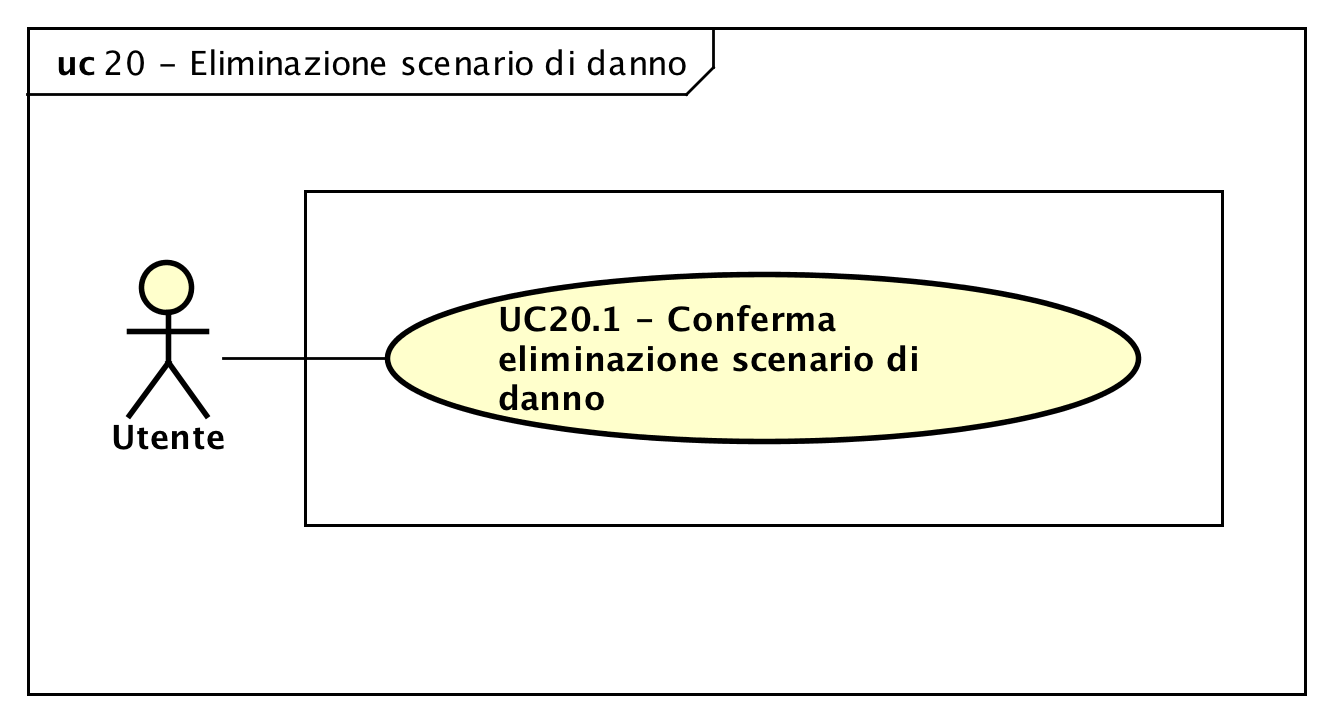
\includegraphics[scale=0.5]{{img/uc20}.png}
\caption{UC20 - Eliminazione scenario di danno}
\end{figure}
\def\arraystretch{1.5}
\rowcolors{2}{D}{P}
\begin{tabularx}{\textwidth}{l|p{0.7\textwidth}}
\rowcolor{I} \multicolumn{2}{c}{\color{white}\textbf{UC20 - Eliminazione scenario di danno}} \\
\toprule
\endhead
\textbf{Attori} & Utente\\
\textbf{Descrizione} & l'utente elimina uno scenario\\
\textbf{Pre-condizione} & l'utente ha aperto l'applicazione; è stato inserito almeno uno scenario; l'utente ha selezionato uno scenario\\
\textbf{Post-condizione} & lo scenario è stato eliminato\\
\textbf{Scenario principale} & \vspace{-1.2em}\begin{enumerate}[leftmargin=*,noitemsep,nosep]
\item \nameref{sssec:UC20.1}.
\end{enumerate}\\
\textbf{Scenari alternativi} & \vspace{-1.2em}\begin{itemize}[leftmargin=*,noitemsep,nosep]
\item \nameref{sssec:UC20.2}.
\end{itemize}\\
%\textbf{Generalizzazioni} &  \\
\bottomrule
\end{tabularx}
\subsection{UC20.1 - Conferma eliminazione scenario di danno}
\label{sssec:UC20.1}
\def\arraystretch{1.5}
\rowcolors{2}{D}{P}
\begin{tabularx}{\textwidth}{l|p{0.7\textwidth}}
\rowcolor{I} \multicolumn{2}{c}{\color{white}\textbf{UC20.1 - Conferma eliminazione scenario di danno}} \\
\toprule
\endhead
\textbf{Attori} & Utente\\
\textbf{Descrizione} & l'utente conferma l'eliminazione dello scenario di danno\\
\textbf{Pre-condizione} & il sistema offre la possibilità di confermare l'eliminazione dello scenario di danno\\
\textbf{Post-condizione} & lo scenario di danno è stato eliminato\\
\textbf{Estensioni} & \vspace{-1.2em}\begin{itemize}[leftmargin=*,noitemsep,nosep]
\item \nameref{sssec:UC20.2}.
\end{itemize}\\
%\textbf{Generalizzazioni} &  \\
\bottomrule
\end{tabularx}
\subsection{UC20.2 - Interruzione eliminazione scenario di danno}
\label{sssec:UC20.2}
\def\arraystretch{1.5}
\rowcolors{2}{D}{P}
\begin{tabularx}{\textwidth}{l|p{0.7\textwidth}}
\rowcolor{I} \multicolumn{2}{c}{\color{white}\textbf{UC20.2 - Interruzione eliminazione scenario di danno}} \\
\toprule
\endhead
\textbf{Attori} & Utente\\
\textbf{Descrizione} & l'utente interrompe l'eliminazione dello scenario di danno\\
\textbf{Pre-condizione} & il sistema offre la possibilità di confermare l'eliminazione dello scenario di danno\\
\textbf{Post-condizione} & lo scenario di danno non è stato eliminato\\
%\textbf{Generalizzazioni} &  \\
\bottomrule
\end{tabularx}
\subsection{UC21 - Avvio analisi di danno}
\label{sssec:UC21}
\def\arraystretch{1.5}
\rowcolors{2}{D}{P}
\begin{tabularx}{\textwidth}{l|p{0.7\textwidth}}
\rowcolor{I} \multicolumn{2}{c}{\color{white}\textbf{UC21 - Avvio analisi di danno}} \\
\toprule
\endhead
\textbf{Attori} & Utente\\
\textbf{Descrizione} & l'utente avvia l'analisi di danno\\
\textbf{Pre-condizione} & l'utente ha aperto l'applicazione\\
\textbf{Post-condizione} & la richiesta di processo dell'analisi di danno è stata inviata al server di calcolo\\
%\textbf{Generalizzazioni} &  \\
\bottomrule
\end{tabularx}
\subsection{UC22 - Visualizzazione risultato analisi di danno su mappa}
\label{sssec:UC22}
\def\arraystretch{1.5}
\rowcolors{2}{D}{P}
\begin{tabularx}{\textwidth}{l|p{0.7\textwidth}}
\rowcolor{I} \multicolumn{2}{c}{\color{white}\textbf{UC22 - Visualizzazione risultato analisi di danno su mappa}} \\
\toprule
\endhead
\textbf{Attori} & Utente\\
\textbf{Descrizione} & l'utente visualizza il risultato dell'analisi di danno sulla mappa\\
\textbf{Pre-condizione} & l'utente ha aperto l'applicazione; i risultati dell'analisi di danno sono stati ricevuti\\
\textbf{Post-condizione} & viene visualizzata su mappa il risultato dell'analisi di danno\\
%\textbf{Generalizzazioni} &  \\
\bottomrule
\end{tabularx}
\subsection{UC23 - Chiusura visualizzazione risultato analisi di danno su mappa}
\label{sssec:UC23}
\def\arraystretch{1.5}
\rowcolors{2}{D}{P}
\begin{tabularx}{\textwidth}{l|p{0.7\textwidth}}
\rowcolor{I} \multicolumn{2}{c}{\color{white}\textbf{UC23 - Chiusura visualizzazione risultato analisi di danno su mappa}} \\
\toprule
\endhead
\textbf{Attori} & Utente\\
\textbf{Descrizione} & l'utente chiude la visualizzazione dell'analisi di danno sulla mappa\\
\textbf{Pre-condizione} & l'utente ha aperto l'applicazione; i risultati dell'analisi di danno sono visualizzati\\
\textbf{Post-condizione} & i risultati dell'analisi di danno non sono più visualizzati sulla mappa\\
%\textbf{Generalizzazioni} &  \\
\bottomrule
\end{tabularx}
\subsection{UC24 - Interazione con la mappa}
\label{sssec:UC24}
\begin{figure}[H]
\centering
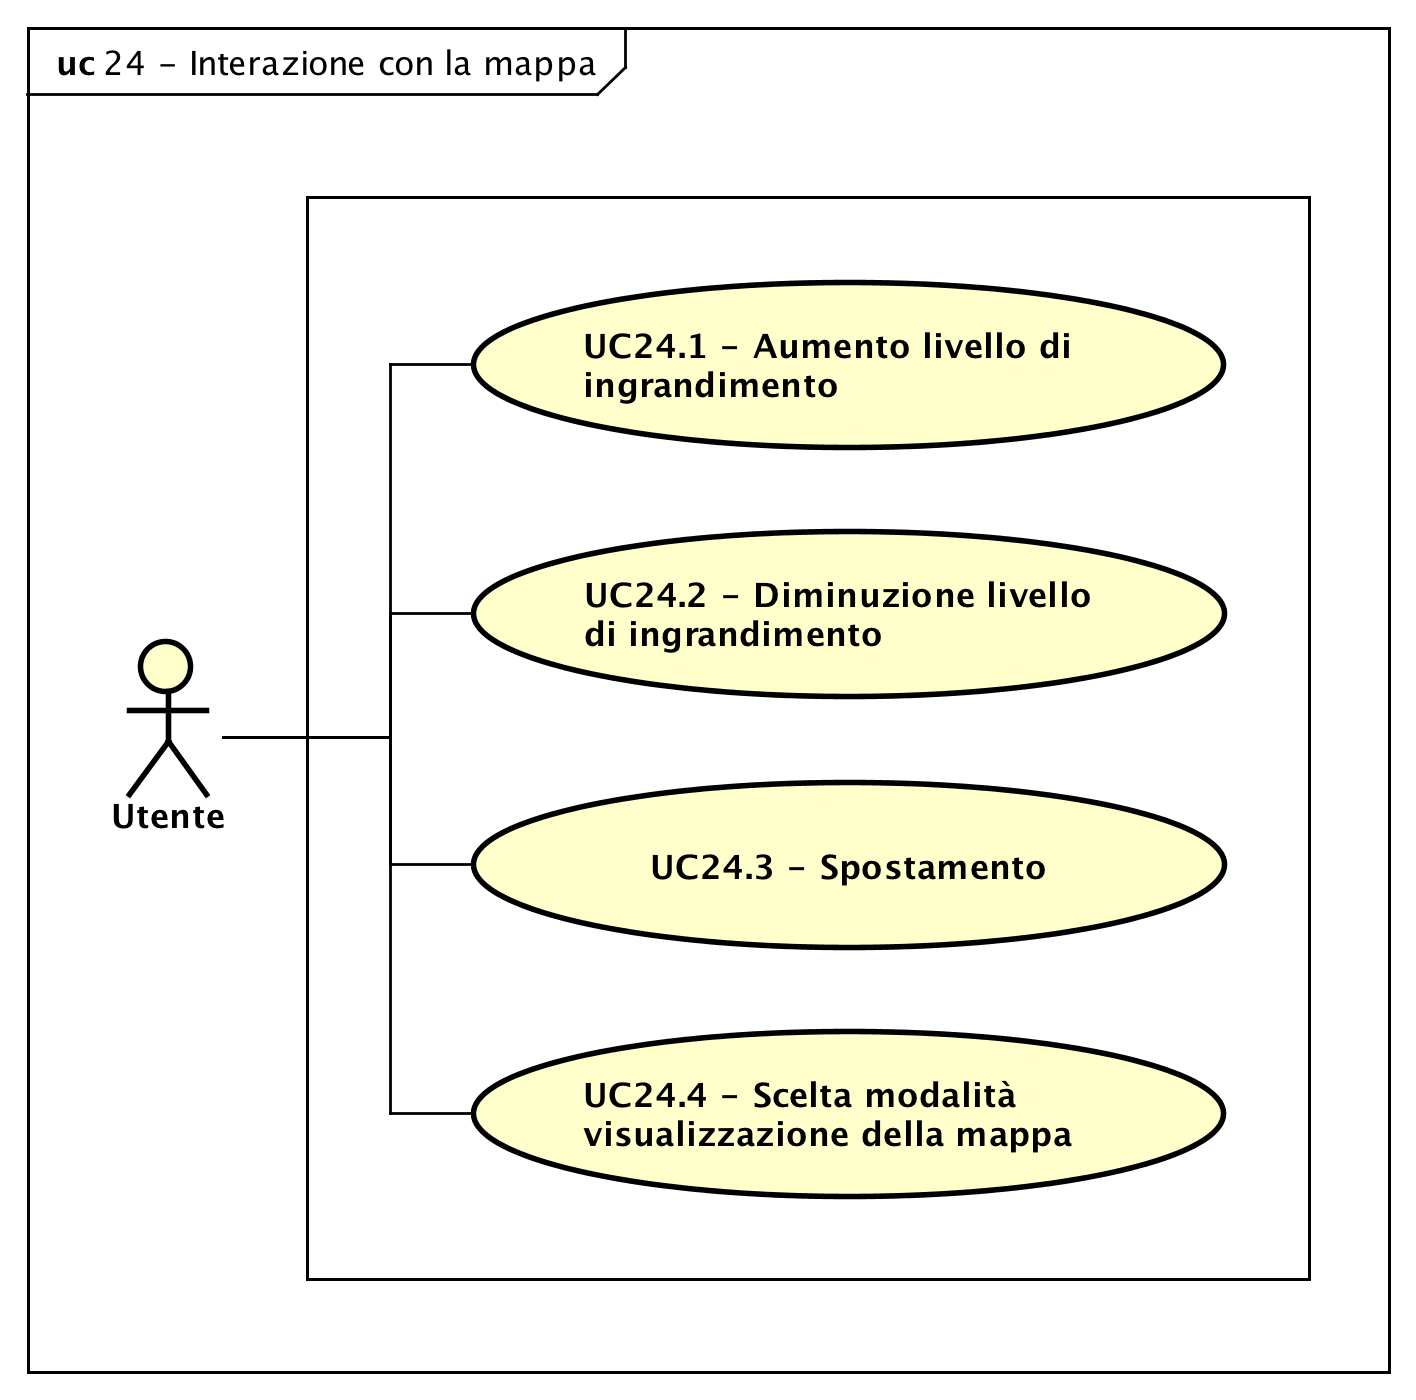
\includegraphics[scale=0.5]{{img/uc24}.png}
\caption{UC24 - Interazione con la mappa}
\end{figure}
\def\arraystretch{1.5}
\rowcolors{2}{D}{P}
\begin{tabularx}{\textwidth}{l|p{0.7\textwidth}}
\rowcolor{I} \multicolumn{2}{c}{\color{white}\textbf{UC24 - Interazione con la mappa}} \\
\toprule
\endhead
\textbf{Attori} & Utente\\
\textbf{Descrizione} & l'utente interagisce con la mappa\\
\textbf{Pre-condizione} & l'utente ha aperto l'applicazione\\
\textbf{Post-condizione} & la mappa ha subito un'interazione\\
\textbf{Scenario principale} & \vspace{-1.2em}\begin{enumerate}[leftmargin=*,noitemsep,nosep]
\item \nameref{sssec:UC24.1};
\item \nameref{sssec:UC24.2};
\item \nameref{sssec:UC24.3};
\item \nameref{sssec:UC24.4}.
\end{enumerate}\\
%\textbf{Generalizzazioni} &  \\
\bottomrule
\end{tabularx}
\subsection{UC24.1 - Aumento livello di ingrandimento}
\label{sssec:UC24.1}
\def\arraystretch{1.5}
\rowcolors{2}{D}{P}
\begin{tabularx}{\textwidth}{l|p{0.7\textwidth}}
\rowcolor{I} \multicolumn{2}{c}{\color{white}\textbf{UC24.1 - Aumenta livello di ingrandimento}} \\
\toprule
\endhead
\textbf{Attori} & Utente\\
\textbf{Descrizione} & l'utente aumenta il livello di ingrandimento della mappa\\
\textbf{Pre-condizione} & l'utente ha aperto l'applicazione; il livello di zoom della mappa può essere aumentato\\
\textbf{Post-condizione} & il livello di zoom della mappa è stato aumentato\\
%\textbf{Generalizzazioni} &  \\
\bottomrule
\end{tabularx}
\subsection{UC24.2 - Diminuzione livello di ingrandimento}
\label{sssec:UC24.2}
\def\arraystretch{1.5}
\rowcolors{2}{D}{P}
\begin{tabularx}{\textwidth}{l|p{0.7\textwidth}}
\rowcolor{I} \multicolumn{2}{c}{\color{white}\textbf{UC24.2 - Diminuzione livello di ingrandimento}} \\
\toprule
\endhead
\textbf{Attori} & Utente\\
\textbf{Descrizione} & l'utente diminuisce il livello di ingrandimento della mappa\\
\textbf{Pre-condizione} & l'utente ha aperto l'applicazione; il livello di zoom della mappa può essere diminuito\\
\textbf{Post-condizione} & il livello di zoom della mappa è stato diminuito\\
%\textbf{Generalizzazioni} &  \\
\bottomrule
\end{tabularx}
\subsection{UC24.3 - Spostamento}
\label{sssec:UC24.3}
\def\arraystretch{1.5}
\rowcolors{2}{D}{P}
\begin{tabularx}{\textwidth}{l|p{0.7\textwidth}}
\rowcolor{I} \multicolumn{2}{c}{\color{white}\textbf{UC24.3 - Spostamento}} \\
\toprule
\endhead
\textbf{Attori} & Utente\\
\textbf{Descrizione} & l'utente sposta la visualizzazione della mappa\\
\textbf{Pre-condizione} & l'utente ha aperto l'applicazione; la visualizzazione della mappa può essere spostata\\
\textbf{Post-condizione} & la visualizzazione della mappa è stata spostata\\
%\textbf{Generalizzazioni} &  \\
\bottomrule
\end{tabularx}
\subsection{UC24.4 - Scelta modalità visualizzazione della mappa}
\label{sssec:UC24.4}
\def\arraystretch{1.5}
\rowcolors{2}{D}{P}
\begin{tabularx}{\textwidth}{l|p{0.7\textwidth}}
\rowcolor{I} \multicolumn{2}{c}{\color{white}\textbf{UC24.4 - Scelta modalità visualizzazione della mappa}} \\
\toprule
\endhead
\textbf{Attori} & Utente\\
\textbf{Descrizione} & l'utente sceglie la modalità di visualizzazione della mappa\\
\textbf{Pre-condizione} & l'utente ha aperto l'applicazione; la modalità di visualizzazione della mappa può essere scelta\\
\textbf{Post-condizione} & la modalità di visualizzazione della mappa è stata scelta\\
%\textbf{Generalizzazioni} &  \\
\bottomrule
\end{tabularx}
\subsection{UC25 - Avvio tutorial}
\label{sssec:UC25}
\def\arraystretch{1.5}
\rowcolors{2}{D}{P}
\begin{tabularx}{\textwidth}{l|p{0.7\textwidth}}
\rowcolor{I} \multicolumn{2}{c}{\color{white}\textbf{UC25 - Avvio tutorial}} \\
\toprule
\endhead
\textbf{Attori} & Utente\\
\textbf{Descrizione} & l'utente avvia il tutorial\\
\textbf{Pre-condizione} & l'utente ha aperto l'applicazione; il tutorial può essere avviato\\
\textbf{Post-condizione} & il tutorial è stato avviato\\
%\textbf{Generalizzazioni} &  \\
\bottomrule
\end{tabularx}
\subsection{UC26 - Avvio assistente vocale}
\label{sssec:UC26}
\def\arraystretch{1.5}
\rowcolors{2}{D}{P}
\begin{tabularx}{\textwidth}{l|p{0.7\textwidth}}
\rowcolor{I} \multicolumn{2}{c}{\color{white}\textbf{UC26 - Avvio assistente vocale}} \\
\toprule
\endhead
\textbf{Attori} & Utente\\
\textbf{Descrizione} & l'utente avvia l'assistente vocale\\
\textbf{Pre-condizione} & l'utente ha aperto l'applicazione; l'assistente vocale può essere avviato\\
\textbf{Post-condizione} & l'assistente vocale è stato avviato\\
%\textbf{Generalizzazioni} &  \\
\bottomrule
\end{tabularx}
